% Modelo de Dissertação do Mestrado em Informática da PUC - Alterado para cumprir a normalização de 2011
%\documentclass[a4paper,brazil,ruledheader,normaltoc,capchap]{abnt}

% Para impressão frente e verso (normalização 2011)
\documentclass[a4paper,brazil,ruledheader,normaltoc,capchap,twoside,openany]{abnt_pucmg_utf8}

% Não esquecer das alterações no arquivo abnt.cls
% Se estiver usando o Kile no Ubuntu o arquivo fica armazenado em /usr/share/texmf/tex/latex/abntex.
% Comentar a linha 967 
% \vspace*{30pt}% - Linha comentada para reduzir o espaçamento entre o topo da página e o título \chapter
% Alterar a linha 1143
% \vspace*{-30pt} % - Parâmetro alterado de 30pt para -30pt para reduzir o espaçamento entre o top da página e o título do apêndice
% Alterar a linha 985
%\vspace*{-30pt}\par % - Parâmetro alterado de 0pt para -30pt para reduzir o espaçamento entre o top da página e o título \chapter*
% Alterar a linha 991
% Parâmetro alterado de 45pt para 30pt para reduzir o espaçamento entre o texto e o título \chapter*

% Não esquecer das alterações no arquivo acronym.sty
% Se estiver usando o Kile no Ubuntu o arquivo fica armazenado em /usr/share/texmf-texlive/tex/latex/acronym
% Alterar a linha 225
%\item[\protect\AC@hypertarget{#1}{\acsfont{\normalfont{#2}}} --] #3% - Inserir separador entre acrônimo/descrição e remover o negrito com o normalfont

% Pacote para definir explicitamente as margens das páginas
\usepackage[a4paper,left=3cm,right=2cm,top=3cm,bottom=2cm]{geometry}

%\usepackage{units}
% Utilize da seguinte forma \unit[78,6]{mA}

% Pacote para gerenciar siglas
\usepackage[printonlyused]{acronym}

% Merge em duas células (linhas diferentes)
\usepackage{multirow}

% Pacote para citação e referências seguindo ABNT no sistema (AUTOR, Data)
%\usepackage[alf, bibjustif,abnt-emphasize=bf]{abntcite}
\usepackage[alf, abnt-emphasize=em, abnt-thesis-year=title]{abntcite}
% @article An article from a journal or magazine 
% @inproceedings An article in a conference proceedings
% Força que o tipo de ênfase no nome do simpósio seja em caixa alta
\renewcommand{\emph}{\textsc}

%Diagrama de Classe
\usepackage{plantuml}

% Pacote para múltiplos arquivos .bib
%\usepackage{multibib}
%\newcites{pub}{Refer\^encias das publica\c{c}\~oes}
% Pacote de adequação do formato ABNT para normas da PUCMinas
\usepackage{abnt-PPGInf-PUCMG}

% Pacotes utilitários
\usepackage{graphicx}

% Pacote para fixar a figura no local desejado
\usepackage{float}

% Pacote para adicionar simbolos as informações de rodapé
\usepackage[symbol]{footmisc}

\usepackage[all]{xy}
%\usepackage[tight]{subfigure}	% Permite a criação de subfiguras
\usepackage{url,amsmath}	% Permite melhorias na codificação de fórmulas
%\usepackage{amsthm}		% Permite melhorias na escrita de teoremas
\usepackage{amssymb}		% Permite utlização de simbolos matemáticos avançados

\usepackage[portuguese, linesnumbered, ruled, vlined]{algorithm2e}
\usepackage{algorithmic} 	% para algoritmos
\usepackage{listings} 		% para importação de código-fonte

% Alterar o espaçamento da margem no algoritmo
\setlength{\algomargin}{1em}

\usepackage{setspace}

% Pacote para rotação de tabelas/figuras
\usepackage{rotating}

% Pacotes para criação de cronograma/tabela colorida
\usepackage{color}
\usepackage{array}
\usepackage{longtable}
\usepackage{colortbl}
%\definecolor{lightgray}{gray}{0.9}

% Pacote para possibilitar o uso do setboolean para forçar formatos de página diferentes do padrão do documento
\usepackage{ifthen}

% Para inserir captions (nova normalização 2011)
\usepackage[size=normalsize,labelfont=bf,textfont={bf},labelsep=endash]{caption}
\captionsetup[subfloat]{labelfont=bf,textfont={bf}}

% Usado para reduzir espaçamentos entre itens (alíneas, enumerações) com o compactitem
\usepackage{paralist}

% Alterar para sequencial a numeração de figuras e tabelas
\captionsetup{figurewithin=none}
\captionsetup{tablewithin=none}

\setlength{\LTcapwidth}{\textwidth}

% Para o subsubsection aparecer no sumário 
\setcounter{tocdepth}{3}
\setcounter{secnumdepth}{3}

% Para inserir referências via links - não funciona para abntex
%\usepackage[colorlinks=true,pdfstartview=FitV,linkcolor=blue,citecolor=blue,urlcolor=blue,hyperindex,pagebackref=true,pdftex,breaklinks]{hyperref}
%\usepackage[pdftex]{hyperref}

% Para criar lista de gráficos
\floatstyle{plaintop}
\newfloat{grafico}{H}{loq}
\restylefloat*{grafico}
\floatname{grafico}{Gráfico} 

% Para gerar subfiguras usando o subfloat
\usepackage{subfig}
\newsubfloat[position=bottom,listofformat=subsimple]{grafico}

% define estilo de posicionamento na caixa
\newsavebox{\leftfig}
\newsavebox{\rightfig}

%\renewcommand{\ALG@name}{Algoritmo}
%\renewcommand{\listalgorithmname}{Lista de Algoritmos}

% Configuração de código-fonte
\lstset{extendedchars=\true, % permite acentos
 inputencoding=utf8,
 literate={\$}{{\$}}1,
 commentstyle=\it, % deixa os comentários em itálico
 stringstyle=\bf, % não lembro o que faz, mas está funcionando
 belowcaptionskip=5pt, % não lembro o que faz, mas está funcionando
 numbers=left, % coloca a numeração na esquerda
 stepnumber=1, % passos da numeração
 firstnumber=1, % primeira linha
 numberstyle=\tiny, % tamanho da fonte da numeração
 breaklines=true, % permitir quebra de linha
 frame=tb, % borda em cima e em baixo
 basicstyle=\footnotesize, % estilo básico
 stringstyle=\ttfamily, % não lembro o que faz, mas está funcionando
 showstringspaces=false, % não mostrar os espaços
 mathescape, % não lembro o que faz, mas está funcionando
 tabsize=3 % tamanho da tabulação
}
\renewcommand{\lstlistingname}{Código}
\renewcommand{\lstlistlistingname}{Lista de Códigos}
\citeoption{abnt-etal-cite=1, abnt-and-type=e}

% the bibtex style generates this command, but it's not defined
\newcommand{\optionaltextstyle}{}

%%\pdfinfo{%
%%  /Title    (TITULO DA DISSERTACAO)
%%  /Author   (Nome do aluno)
%%  /Creator  (Nome do aluno)
%%  /Producer (Kile - an Integrated LaTeX Environment - %%Version 2.0.85)
%%  /Subject  (Dissertação de Mestrado)
%% /Keywords (Palavras chave)
%%}

% PRÉ-TEXTUAIS %%
\begin{document}

% Para forçar que elementos pré-textuais (da capa até o sumário) sejam impressos no anverso da folha
\setboolean{@twoside}{false}

\autor{Breno Rosa Almeida \\ Gabriel Victor Couto Martins de Paula \\ Luís Antônio de Souza e Sousa \\ Rúbia Coelho de Matos}

% Coloque o título em caixa alta. É o padrão da PUC.
% Vá no arquivo abnt-PPGInf-PUCMG.sty e procure por esse título (linha 575). Altere para o seu título em caixa alta. Isso será utilizado na folha de aprovação.
\titulo{Bridge finding}

%\orientador[Orientador:]{título + nome do orientador}

% Se não tiver, co-orientador, comente a próxima linha.
%\coorientador[Co-orientador:]{Professor}

% Texto
\comentario{Projeto de Bridge finding apresentado na disciplina Teoria dos Grafos e Computabilidade do curso de Engenharia de Software da Pontifícia Universidade Católica de Minas Gerais.}


% Instituição
\instituicao{Engenharia de Software \par Instituto de Ciências Exatas e Informática \par Pontifícia Universidade Católica de Minas Gerais}

% Local
\local{Belo Horizonte}

% Data
\data{2022}
\capa
%Para forçar que a ficha catalográfica seja impressa no verso da folha de aprovação
\setboolean{@twoside}{true}

% Gera a folha de rosto
\folhaderosto

% Ficha catalográfica
%\include{pre-texto/ficha-catalografica}

% Para forçar que elementos pré-textuais (da capa até o sumário) sejam impressos no anverso da folha
\setboolean{@twoside}{false}

% Folha de aprovação
%\include{pre-texto/folha-aprovacao}

% Dedicatória
%\include{pre-texto/dedicatoria}

% Agradecimentos
%\include{pre-texto/agradecimentos}

% Epígrafe
%\include{pre-texto/epigrafe}

% Resumo
% Resumo
\begin{resumo}
% Diminuir espaçamento entre título e texto
\vspace{-1cm}

% Texto do resumo: sem paragrafo, justificado, com espaçamento 1,5 cm
\onehalfspacing

\noindent 


% Espaçamento para as palavras-chave
\vspace*{.75cm}

% Palavras-chave: sem parágrafo, alinhado à esquerda
\noindent Palavras-chave: Matriz de Adjacência, Lista de Adjacência, Caminho Euleriano, Ponte, Conectividade, Biblioteca de Manipulação de Grafos.
% Segunda linha de palavras-chave, com espaçamento.
%\indent\hspace{2cm}Palavra.

\end{resumo}

% Abstract
%% Abstract
\begin{abstract}
% Diminuir espaçamento entre título e texto
\vspace{-1cm}
% Texto do resumo, em inglês: sem paragrafo, justificado, com espaçamento 1,5 cm
\onehalfspacing
\noindent
  Texto do resumo, em ingles.

% Espaçamento para as palavras-chave
\vspace*{.75cm}

% Palavras-chave: sem parágrafo, alinhado à esquerda
\noindent Keywords: . \\
% Segunda linha de palavras-chave, com espaçamento.
%\indent\hspace{1.4cm} Keyword.

\end{abstract}

\makeatletter
\renewcommand\numberline[1]{
	\leftskip 0em
	\rightskip 1.6em
	\parfillskip -\rightskip
	\parindent 0em
	\@tempdima 2.0em
	\vspace{0em} \advance\leftskip \@tempdima \null\nobreak\hskip -\leftskip
	FIGURA \normalfont #1 -- }
\makeatother

% Lista de figuras
%\listoffigures

\makeatletter
\renewcommand\numberline[1]{
	\leftskip 0em
	\rightskip 1.6em
	\parfillskip -\rightskip
	\parindent 0em
	\@tempdima 2.0em
	\vspace{0em} \advance\leftskip \@tempdima \null\nobreak\hskip -\leftskip
	TABELA \normalfont #1 -- }
\makeatother

% Lista de tabelas
%\listoftables

\makeatletter
\renewcommand\numberline[1]{
	\leftskip 0em
	\rightskip 1.6em
	\parfillskip -\rightskip
	\parindent 0em
	\@tempdima 2.0em
	\vspace{0.5em} \advance\leftskip \@tempdima \null\nobreak\hskip -\leftskip
	GRÁFICO \normalfont #1 -- }
\makeatother

% Lista de graficos
%\listof{grafico}{Lista de Graficos}

% Lista de siglas
%% Lista de Abreviaturas e Siglas
%\chapter*{Lista de Abreviaturas e Siglas}
\chapter*{Lista de Abreviaturas e Siglas}

% Mantenha sempre em ordem alfabética.

\begin{acronym}
\acro{BER} {\textit{Bit Error Rate}}
\acro{BT} {\textit{Block Tri-diagonal}}
\acro{CG} {\textit{Conjugate Gradient}}
\acro{CSS} {\textit{Chirp Spread Spectrum}}
\acro{DCC-MAC} {\textit{Dynamic Channel Coding} MAC}
\acro{DSSS} {\textit{Direct-sequence spread spectrum}}
\acro{EP} {\textit{Embarrassingly Parallel}}
\acro{FIFO} {\textit{First In, First Out}}
\acro{FT} {\textit{Fast Fourier Transform}}
\acro{IEEE} {\textit{Institute of Electrical and Electronics Engineers}}
\acro{IR-UWB} {\textit{Impulse Radio} UWB}
\acro{IS} {\textit{Integer Sort}}
\acro{LU} {\textit{Lower-Upper Gauss-Seidel}}
\acro{MAC} {\textit{Medium Access Control}}
\acro{MB-OFDM} {\textit{Multi-Band Orthogonal Frequency Division Multiplexing}}
\acro{MG} {\textit{Multi-Grid}}
\acro{MPE} {MPI \textit{Parallel Environment}}
\acro{MPI} {Interface de passagem de mensagem, do inglês \textit{Message Passing Interface}}
\acro{NAS} {NASA \textit{Advanced Supercomputing}}
\acro{NOAH} {\textit{No Ad-Hoc Routing Agent}} 
\acro{NS-2} {\textit{Network Simulator} 2}
\acro{NoCs} {Redes-em-Chip, do inglês \textit{Networks-on-Chip}}
\acro{NPB} {NAS \textit{Parallel Benchmark}}
\acro{OpenMP} {Multi-processamento aberto, do inglês \textit{Open Multi-Processing}}
\acro{PHY} {\textit{Physical Layer}}
\acro{PPM} {\textit{Pulse-Position Modulation}}
\acro{SP} {\textit{Scalar Penta-diagonal}}
\acro{TH} {\textit{Time Hopping}}
\acro{THS} {\textit{Time Hopping Sequence}}
\acro{UDP}{\textit{User Datagram Protocol}}
\acro{UWB} {\textit{Ultra Wide Band}}
\acro{WiNoCs} {Redes-em-Chip Sem Fio, do inglês \textit{Wireless Networks-on-Chip}}
\acro{WLAN} {Rede Local Sem Fio, do inglês \textit{Wireless Local Area Network}}
\acro{WPAN} {Rede de Área Pessoal Sem Fio, do inglês \textit{Wireless Personal Area Network}}
\end{acronym}

\makeatletter
\renewcommand\numberline[1]{#1\hspace{0.8em}}
\makeatother

% Altera para espaçamento simples a partir daqui
\singlespacing

% Sumário
\tableofcontents

% Altera para espaçamento 1,5 a partir daqui
\onehalfspacing

%% TEXTUAIS 
% Para forçar que elementos textuais e pós-textuais sejam impressos no anverso e verso das folhas
\setboolean{@twoside}{true}
% Altere o número da página para o correto. Conte todas as páginas frente e verso, menos a capa, nclusive a ficha catalográfica até a página do primeiro capítulo.
\setcounter{page}{1}

% Capítulos
% Para forçar que o capítulo de introdução comece no anverso
\setboolean{@openright}{true}
\chapter{Introdução}
\label{intro}


%Contexto - dois a quatro parágrafos 

%Problema 

%Justificativa


%Este trabalho está organizado da seguinte forma. A seção~\ref{sec:Obj} asdadas  dasda. O capítulo~\ref{revisao} apresenta o referencial teórico usado neste trabalho. O capítulo~\ref{metodo} descreve os procedimentos metodológicos  ...


\section{Objetivos}
%\addcontentsline{toc}{chapter}{Objetivos}
\label{sec:Obj}

Trabalho tem como objetivo fazer.
%O objetivo geral deste projeto é ...

\subsection{Objetivos específicos}

% Os objetivos específicos deste projeto são:
% \begin{enumerate}
%     \item asdasd
%     \item asdasd
%     \item asd
% \end{enumerate}
% Os demais capítulos não precisam começar no anverso
\setboolean{@openright}{false}
\chapter{Revisão bibliográfica}

Este capítulo apresenta ``asdasd lkjlaskjd alskdjas asd  sdoiosfugoigodf sps uh psdh sdip hdsoiph osdif. osidf jsodfij woerui jdsf hlieguh ioduhg eirh dlfigh epogri çsaodfji açefj sçofi jaçefoij açewfoi jwoçpefi jweaoifj''.

\begin{citacao}
sodisodfi osigu woriu çdoig çsoigj eçorig oeçrgji oier.  psdh sdip hdsoiph osdasda qwre qwed asd qe asd q asd q asd qw asd q asd qe asd qwe asd qwe asd if. osidf jsodfij woerui jdsf hlieguh ioduhg eirh dlfigh epogri çsaodfji açefj sçofi jaçefoij açewfoi jwoçpefi jweaoifj. (AUTOR, ano).
\end{citacao}


\section{xxxx}


\section{xxxx}
\chapter{Desenvolvimento}
\label{metodo}

\section{Biblioteca de manipulação de grafos}
Como primeira etapa foi desenvolvida uma biblioteca de manipulação de grafos que será utilizada futuramente nas próximas
etapas.

A biblioteca de manipulação é composta por um conjunto de funções e métodos que manipulam tanto um grafo representado
em matriz, quanto um grafo representado por lista de adjacência.

Para um bom design de solução, que fosse reutilizável e compreensível, foi utilizada a linguagem Java como principal
ferramenta. A arquitetura desenvolvida para a biblioteca, nos dá a liberdade para escolher qual estrutura de dados
manipular e utilizar de módulos de geração, leitura e salvamento de grafos de maneira separada.

A Biblioteca como um todo é composta por duas classes principais que guardam as estruturas de dados de Grafos em matriz
e em lista de adjacência. A primeira classe é chamada de GraphMatrix, responsável por manipular e armazenar um grafo
não-direcionado em uma matriz de N linhas por N colunas tal que N é o número de vértices do grafo. A segunda classe
se chama apenas Graph e ela herda todas as características de GraphMatrix. Graph, é responsável por manipular e
armazenar tanto grafo em matriz, quanto o grafo em lista de adjacência.

Além das classes principais, existem outros dois módulos que auxiliam nos testes e desenvolvimento. Sendo o primeiro
deles chamado de GraphIO, utilizado na leitura e salvamento de grafos em arquivos no formato Pajek NET, e o segundo
módulo, chamado de GraphGenerator, responsável por gerar grafos com base na quantidade de vértices, número mínimo de
grau por vértice e número máximo de grau por vértice.

Para garantir que todos os algoritmos estão funcionando corretamente e retornando resultados esperados, foram
desenvolvidas baterias de teste para cada uma das funções do sistema. Assim, é possível ter certeza e confiar que
tanto o processamento que ocorre nas matrizes, quanto os que ocorrem nas listas entregam os mesmos resultados de
adição e remoção de arestas, ponderação de vértices e arestas, e para todas as outras funções. Os testes foram
escritos utilizando a biblioteca Junit do próprio Java.

A Organização de todo o sistema pode ser representada pelo seguinte diagrama de classe:

\begin{figure}[H]
    % Alterar espaçamentos antes e depois do caption
    \setlength{\abovecaptionskip}{0pt}
    \setlength{\belowcaptionskip}{0pt}
    % Caption
    \caption[Diagrama de Classe]{Diagrama de Classe}
    \centering
    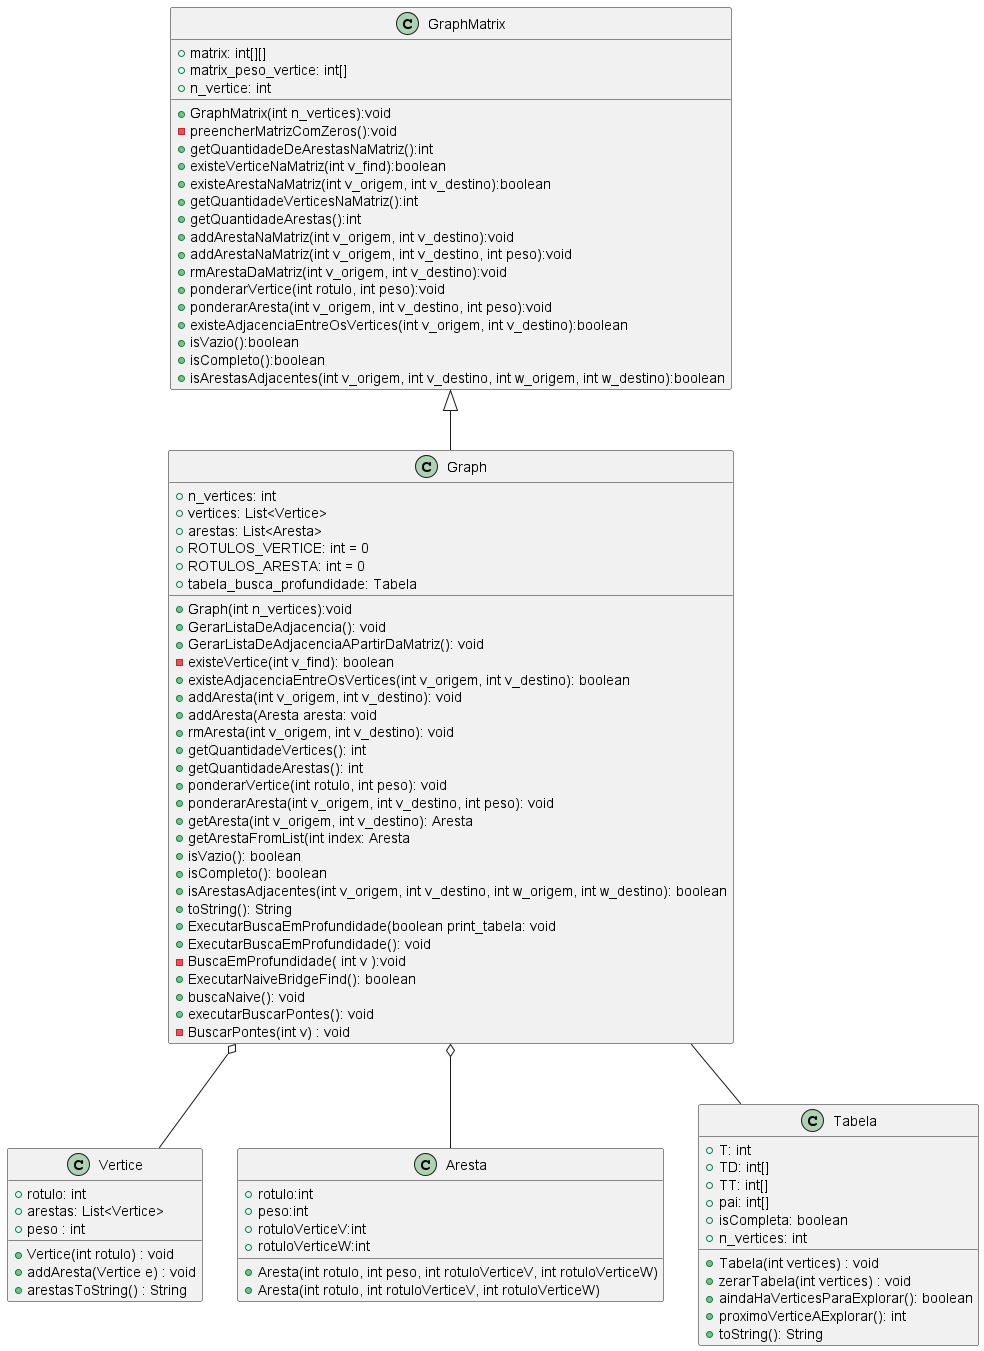
\includegraphics[width=1\textwidth]{DiagramaDeClasse/DiagramaDeClasse.png}
    % Caption centralizada
    \captionsetup{justification=centering}
    %\captionfont{\small{\textbf{\\Fonte: }}}}	
    \label{fig:DiagramaDeClasse}
\end{figure}

\section{Ciclo Euleriano}

Passa uma única vez por cada aresta no grafo, partindo e chegando a um mesmo vértice.

\begin{itemize}
    \item Para haver um ciclo euleriano, todo vértice deve ter grau par, como já discutimos.
\end{itemize}

O algoritmo de Fleury, proposto em 1883, utiliza um grafo reduzido induzido pelas arestas ainda não marcadas

\begin{itemize}
    \item Inicialmente todas as arestas estão não marcadas.
    \item As arestas vão sendo "marcadas", ou removidas do grafo, a medida em que vão sendo inseridas no ciclo
\end{itemize}

Regra da ponte: se uma aresta {v, w} é uma ponte no grafo reduzido, então {v, w} só deve ser escolhida caso não haja outra opção.

\section{Algoritmo de Fleury}

Passo a passo para um grafo não dirigido e não valorado

\begin{enumerate}
    \item Verifique se o grafo apresenta as condições para ter um ciclo euleriano
    \item Caso positivo, escolha um vértice V1 para começar.
    \item Entre os vértices adjacentes a V1, faça
          \begin{enumerate}
              \item Se há apenas um vértice como opção, escolha este como V2.
              \item Se há mais de um vértice possível, escolha um V2 apropriado dentre eles (ou seja, um que “não repita a ponte”).
          \end{enumerate}
    \item Remova a aresta (V1, V2).
    \item Se ainda houver arestas não percorridas, volte ao passo 3, partindo agora de V2 (V2 é o novo V1).
    \item Caso contrário, imprima o caminho percorrido.
\end{enumerate}

Exemplos do passo a passo do algoritmo funcionando:

    \label{fig:PassoPasso}
    \begin{subfigure}{.4\textwidth}
		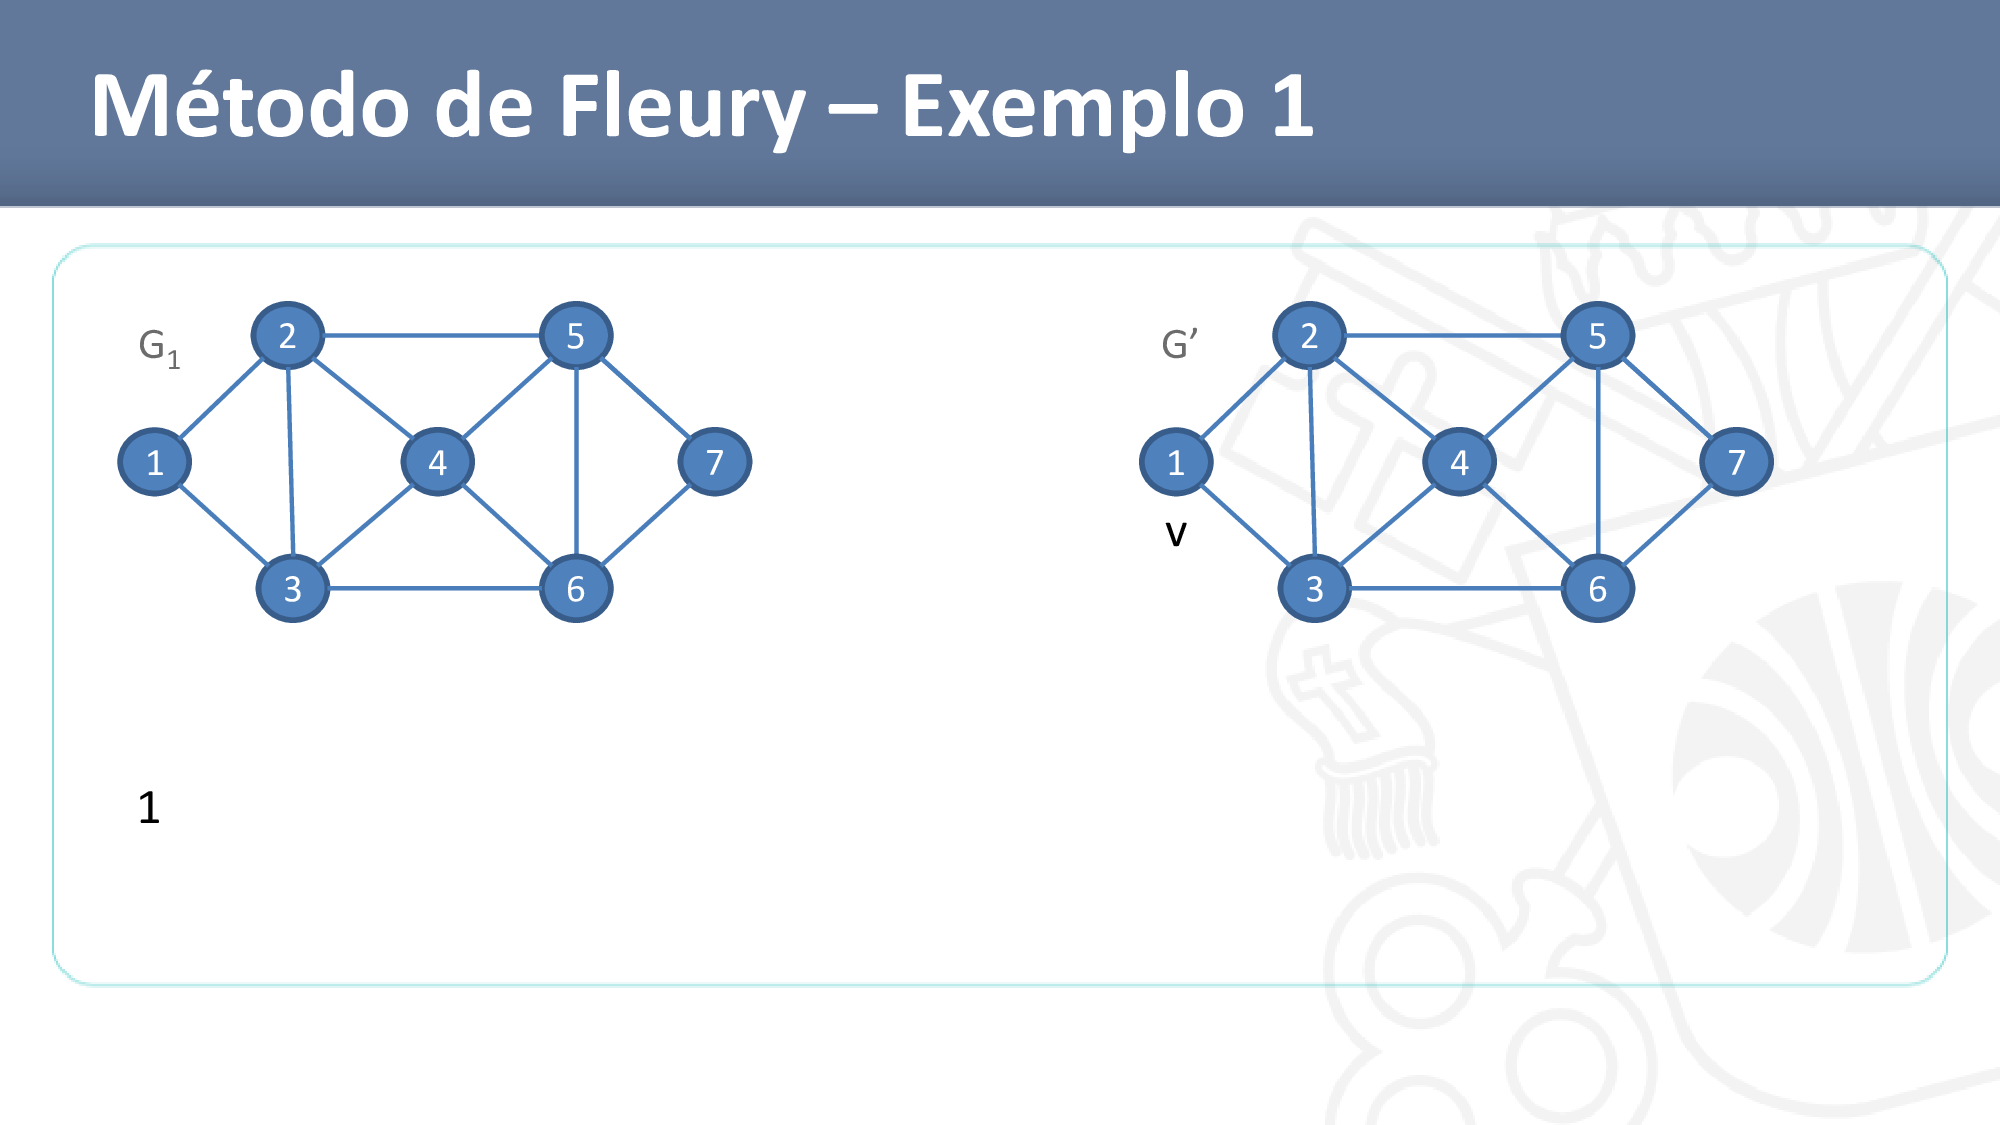
\includegraphics[width=\textwidth]{imagem/graficos/1a1455b7b9174768d1c6a0d41673e79dHTztESkzBtQzsXWu-25.png}
	\end{subfigure}
    \begin{subfigure}{.4\textwidth}
		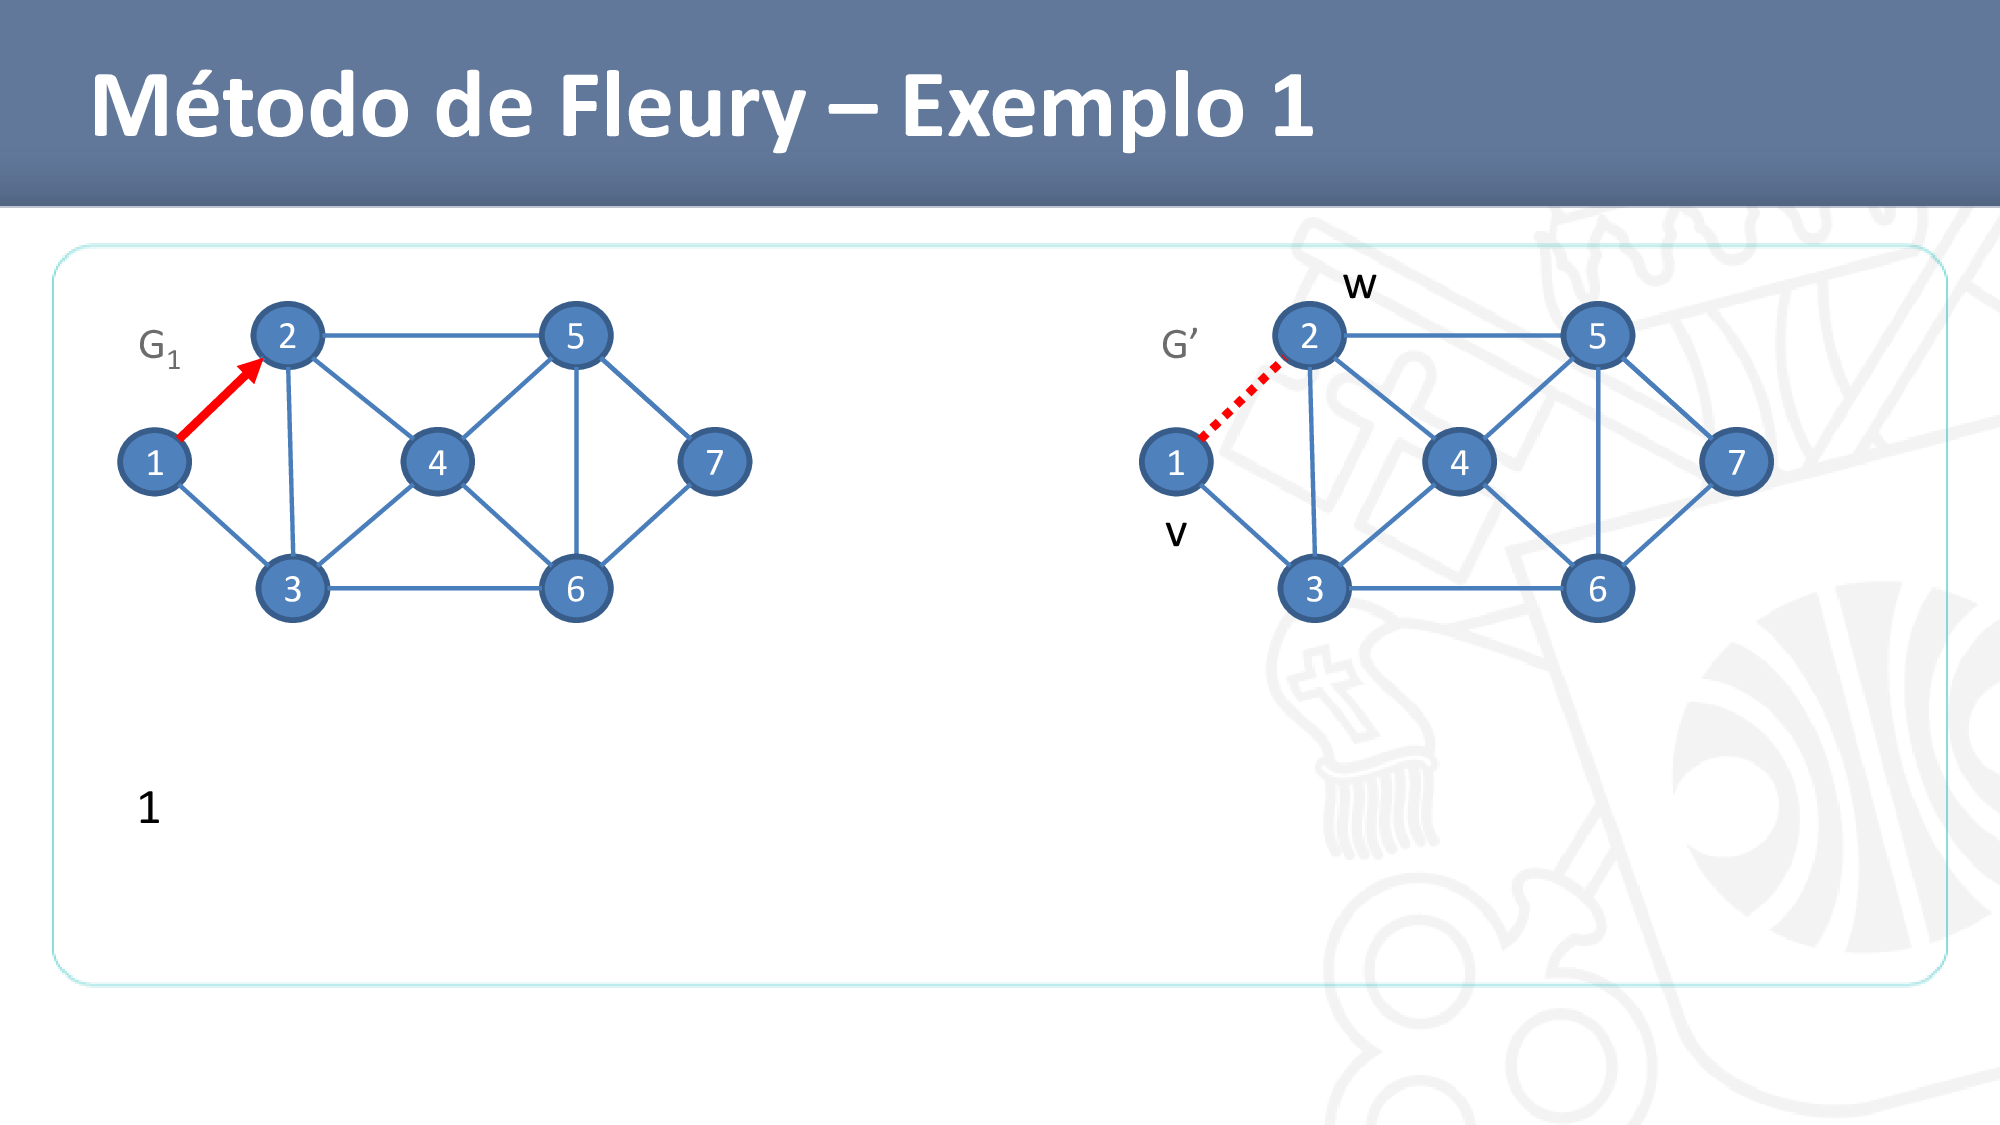
\includegraphics[width=\textwidth]{imagem/graficos/1a1455b7b9174768d1c6a0d41673e79dHTztESkzBtQzsXWu-26.png}
	\end{subfigure}
\begin{figure}[htbp]
    \begin{subfigure}{.4\textwidth}
		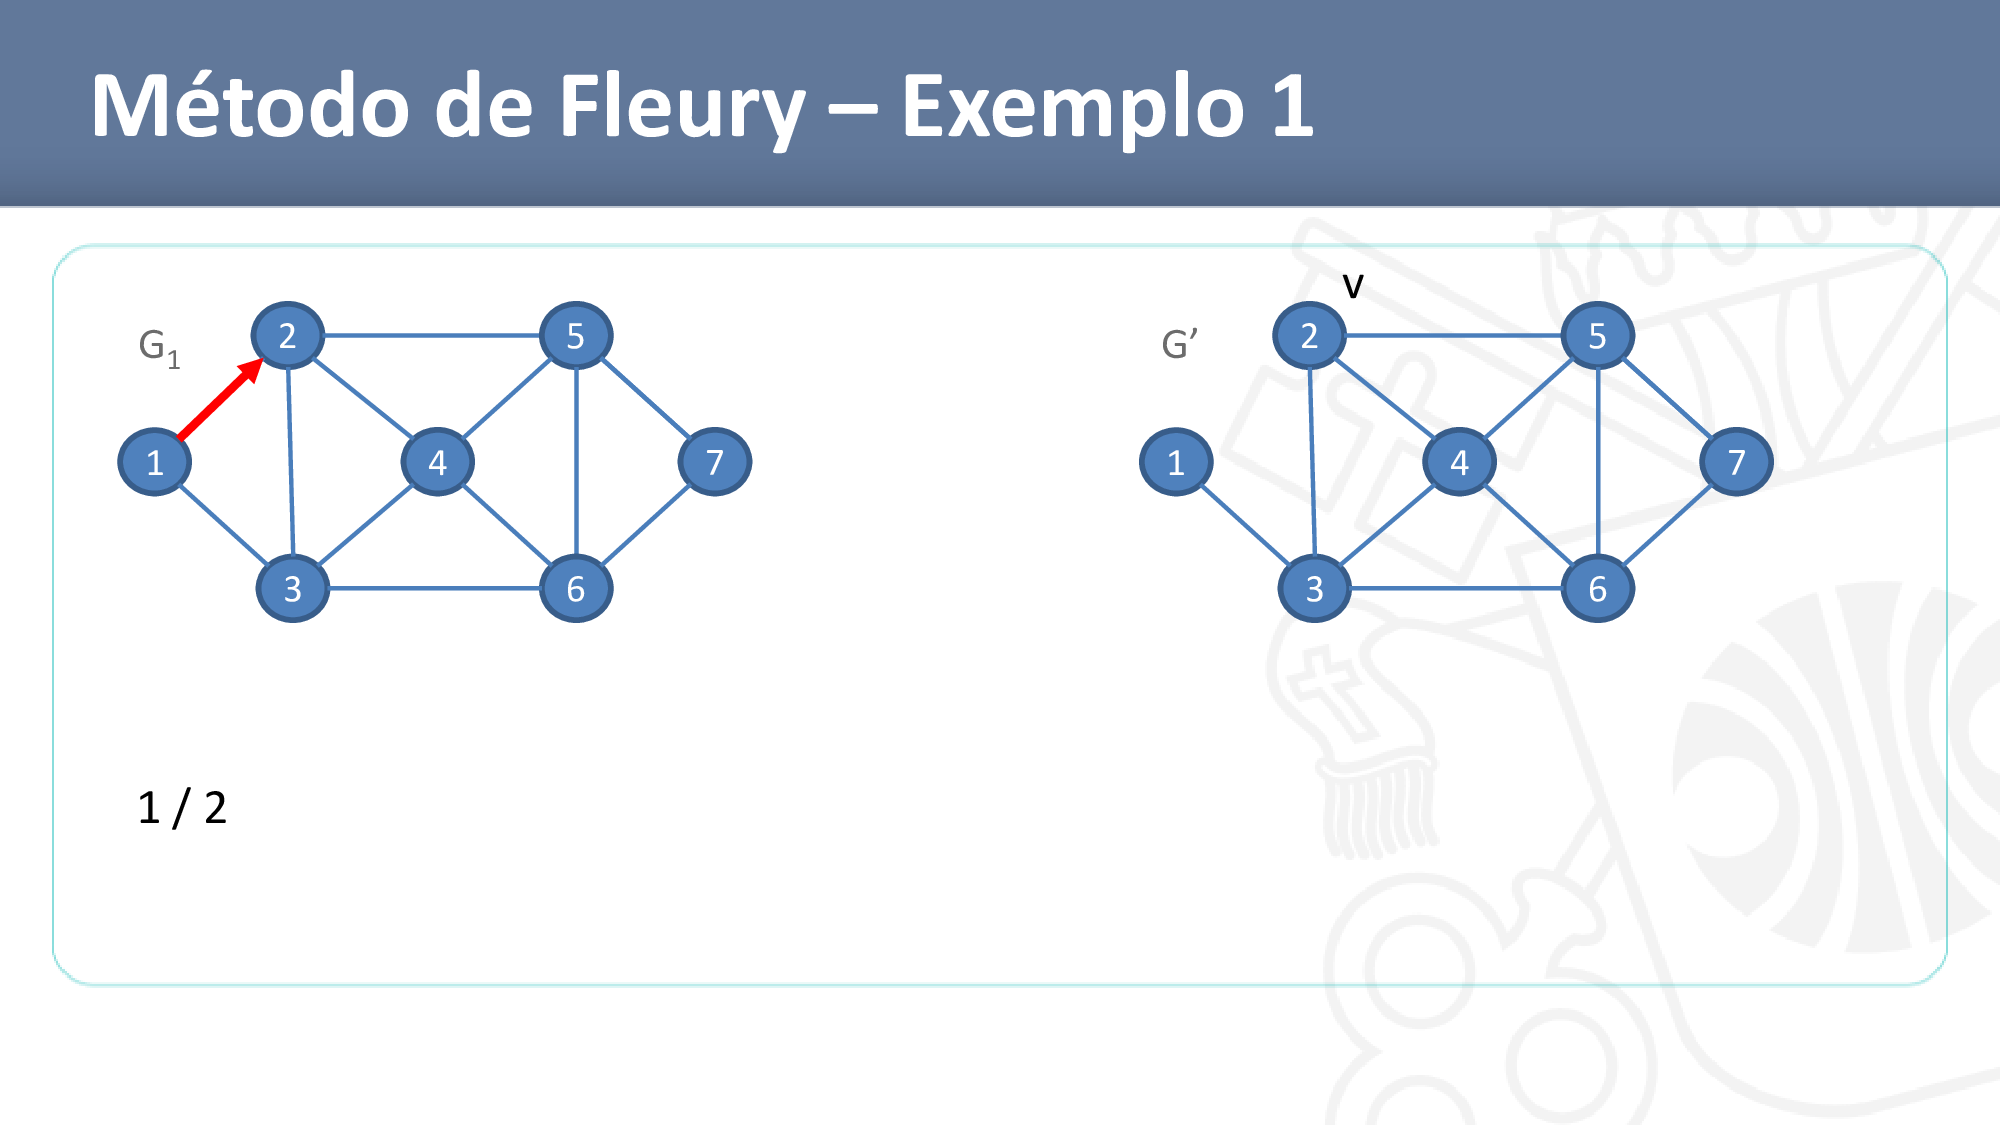
\includegraphics[width=\textwidth]{imagem/graficos/1a1455b7b9174768d1c6a0d41673e79dHTztESkzBtQzsXWu-27.png}
	\end{subfigure}
    \begin{subfigure}{.4\textwidth}
		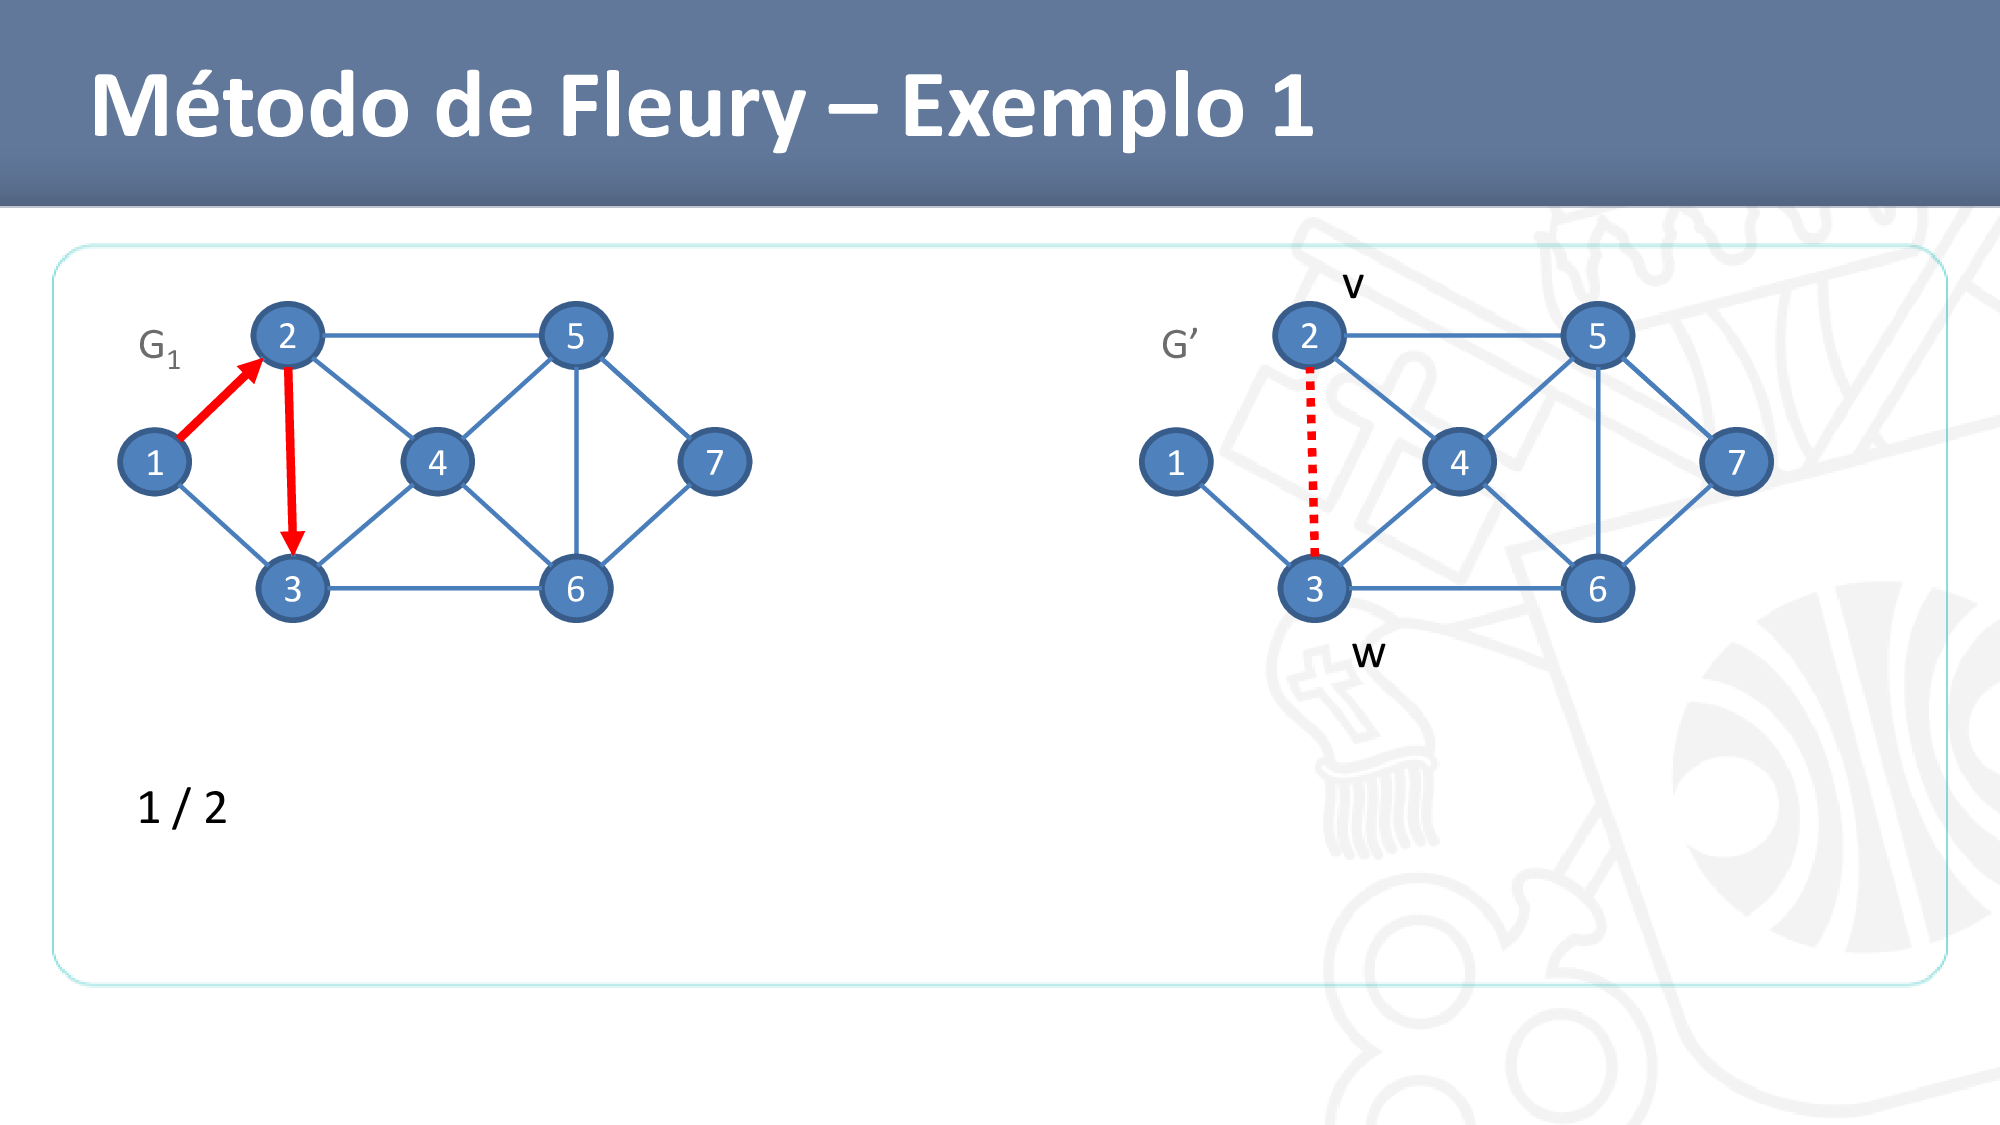
\includegraphics[width=\textwidth]{imagem/graficos/1a1455b7b9174768d1c6a0d41673e79dHTztESkzBtQzsXWu-28.png}
	\end{subfigure}
\end{figure}
\begin{figure}[htbp]
    \begin{subfigure}{.4\textwidth}
		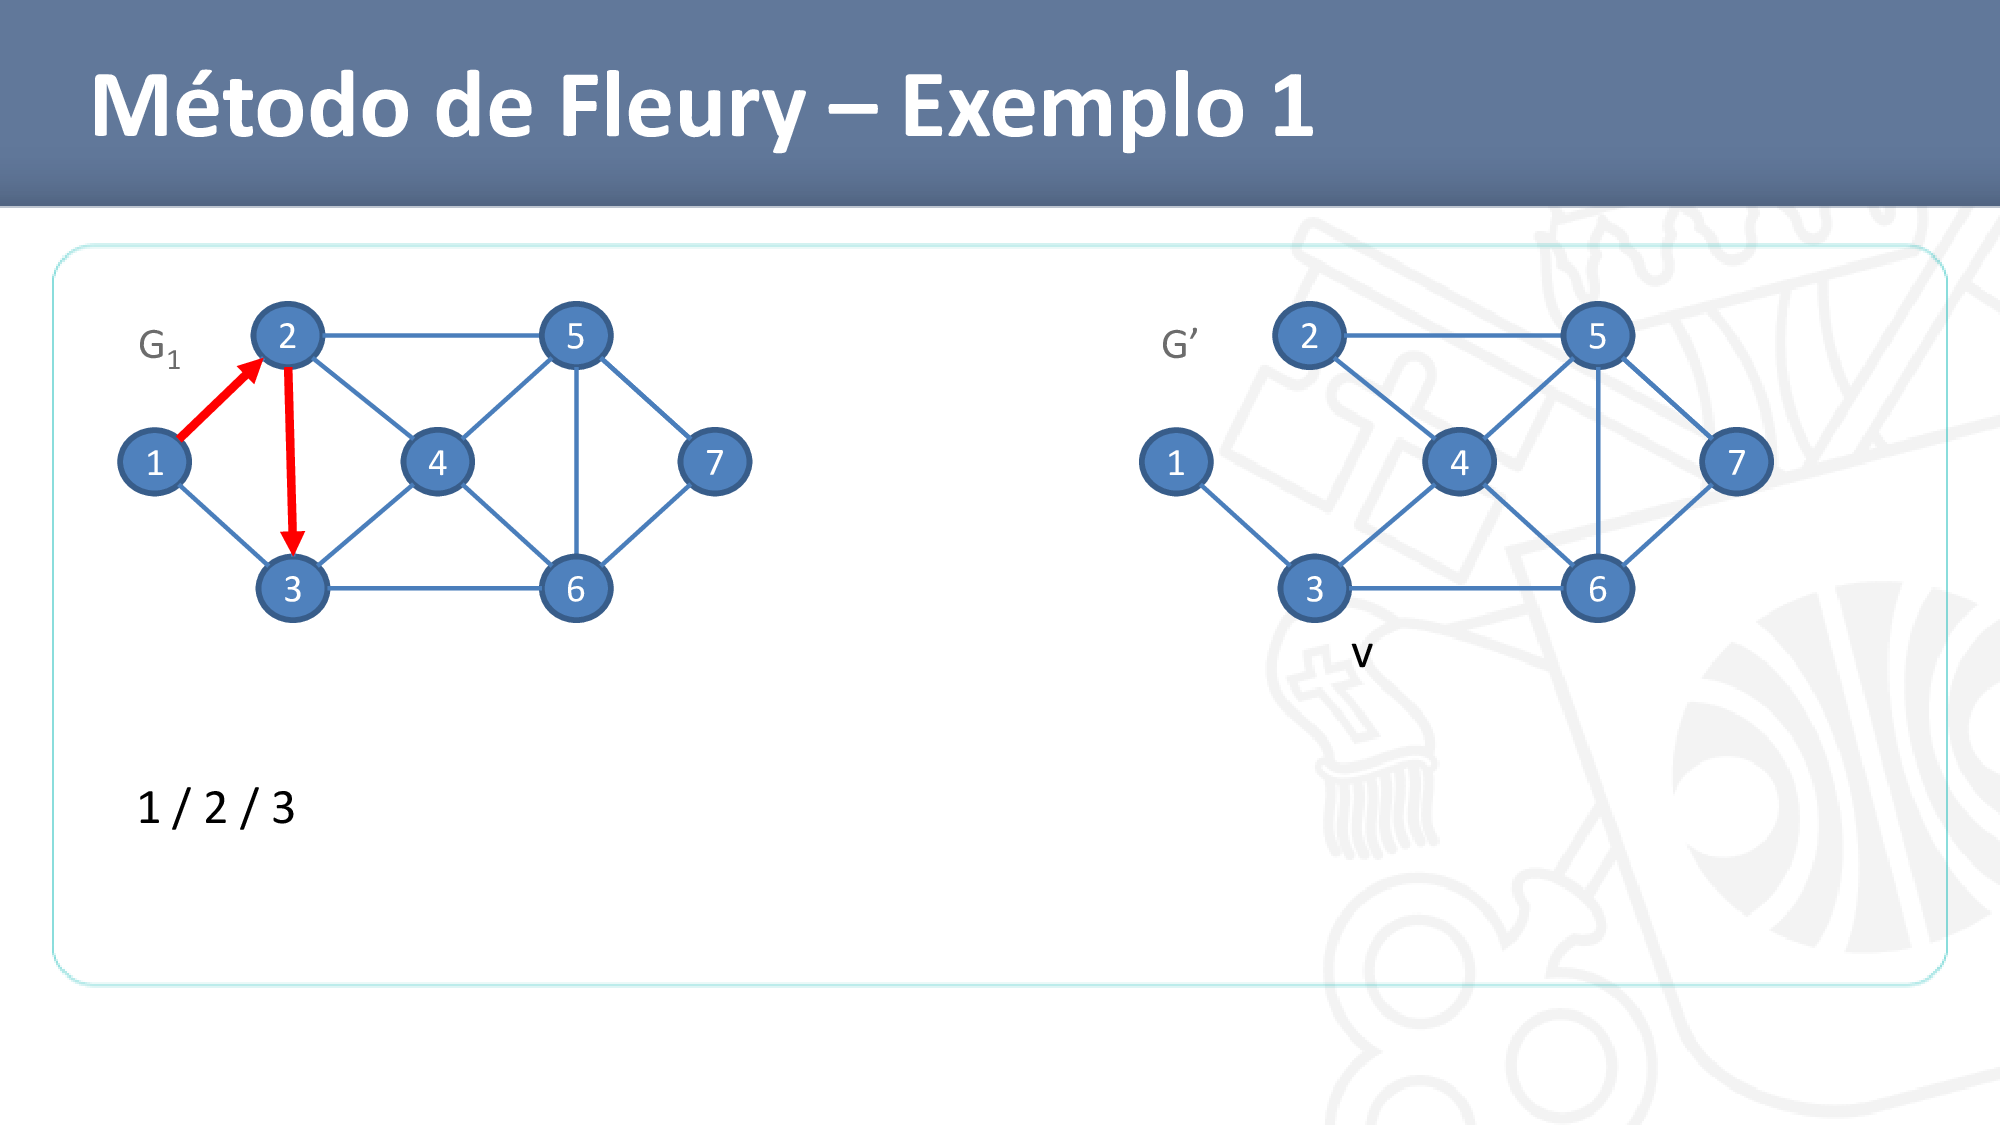
\includegraphics[width=\textwidth]{imagem/graficos/1a1455b7b9174768d1c6a0d41673e79dHTztESkzBtQzsXWu-29.png}
	\end{subfigure}
    \begin{subfigure}{.4\textwidth}
		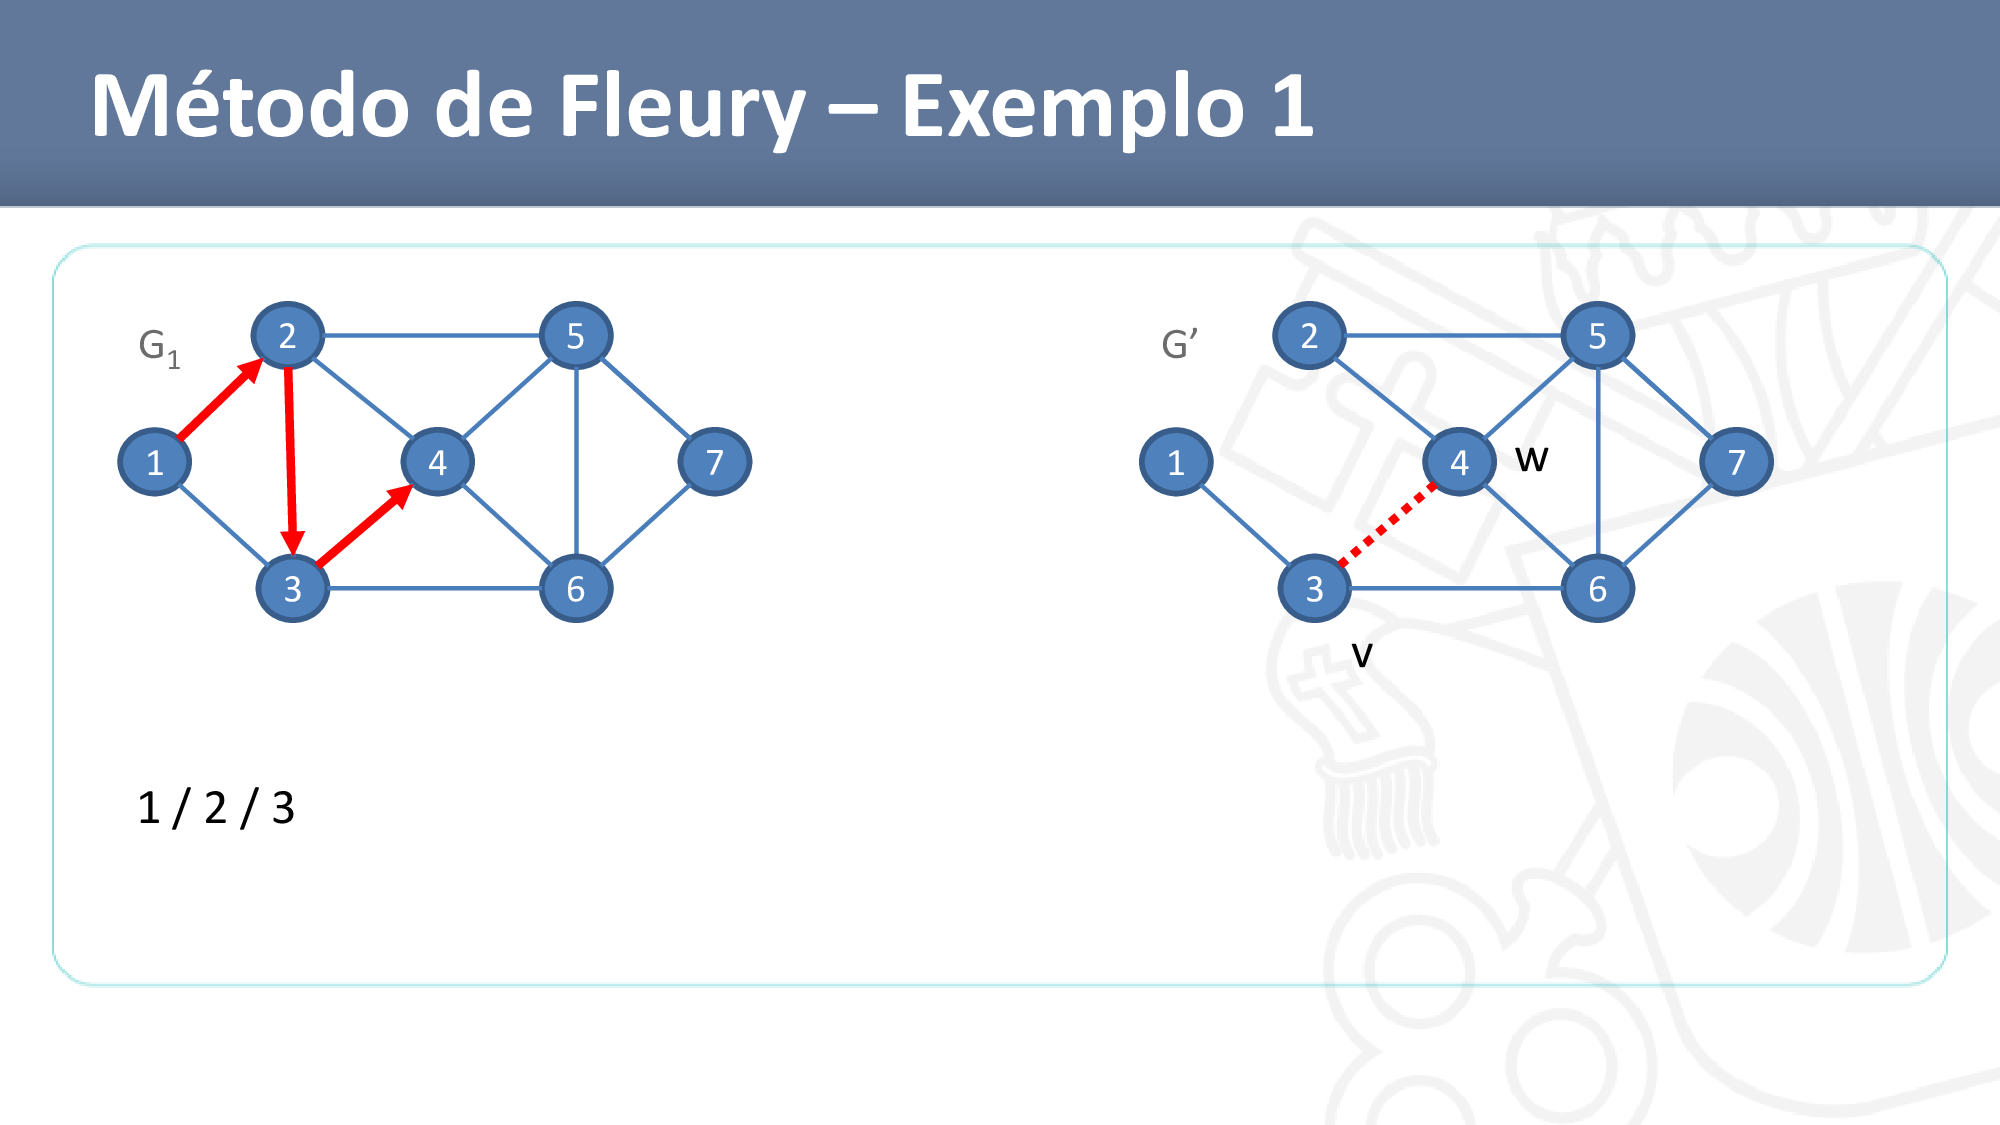
\includegraphics[width=\textwidth]{imagem/graficos/1a1455b7b9174768d1c6a0d41673e79dHTztESkzBtQzsXWu-30.png}
	\end{subfigure}
\end{figure} 
\begin{figure}[htbp]
    \begin{subfigure}{.4\textwidth}
		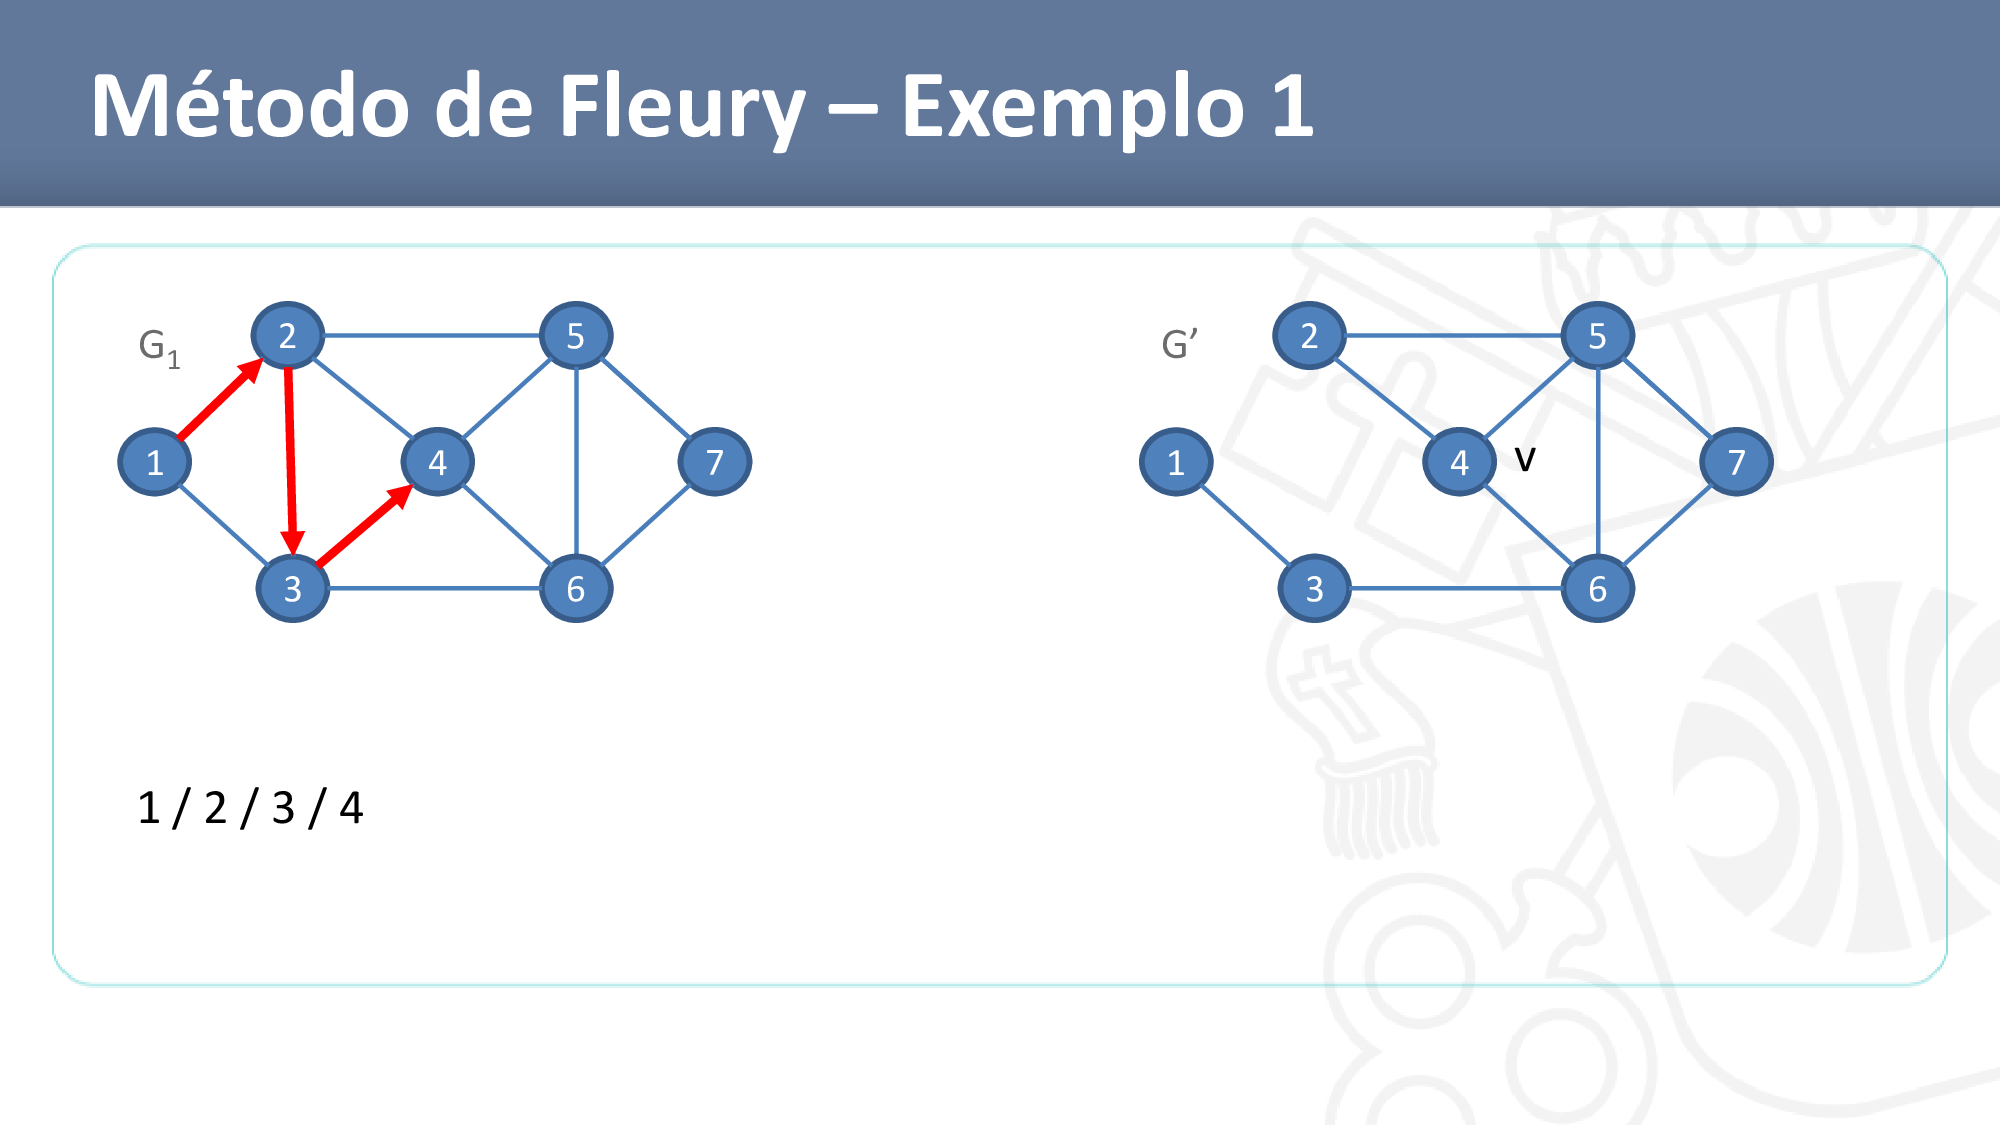
\includegraphics[width=\textwidth]{imagem/graficos/1a1455b7b9174768d1c6a0d41673e79dHTztESkzBtQzsXWu-31.png}
	\end{subfigure} 
    \begin{subfigure}{.4\textwidth}
		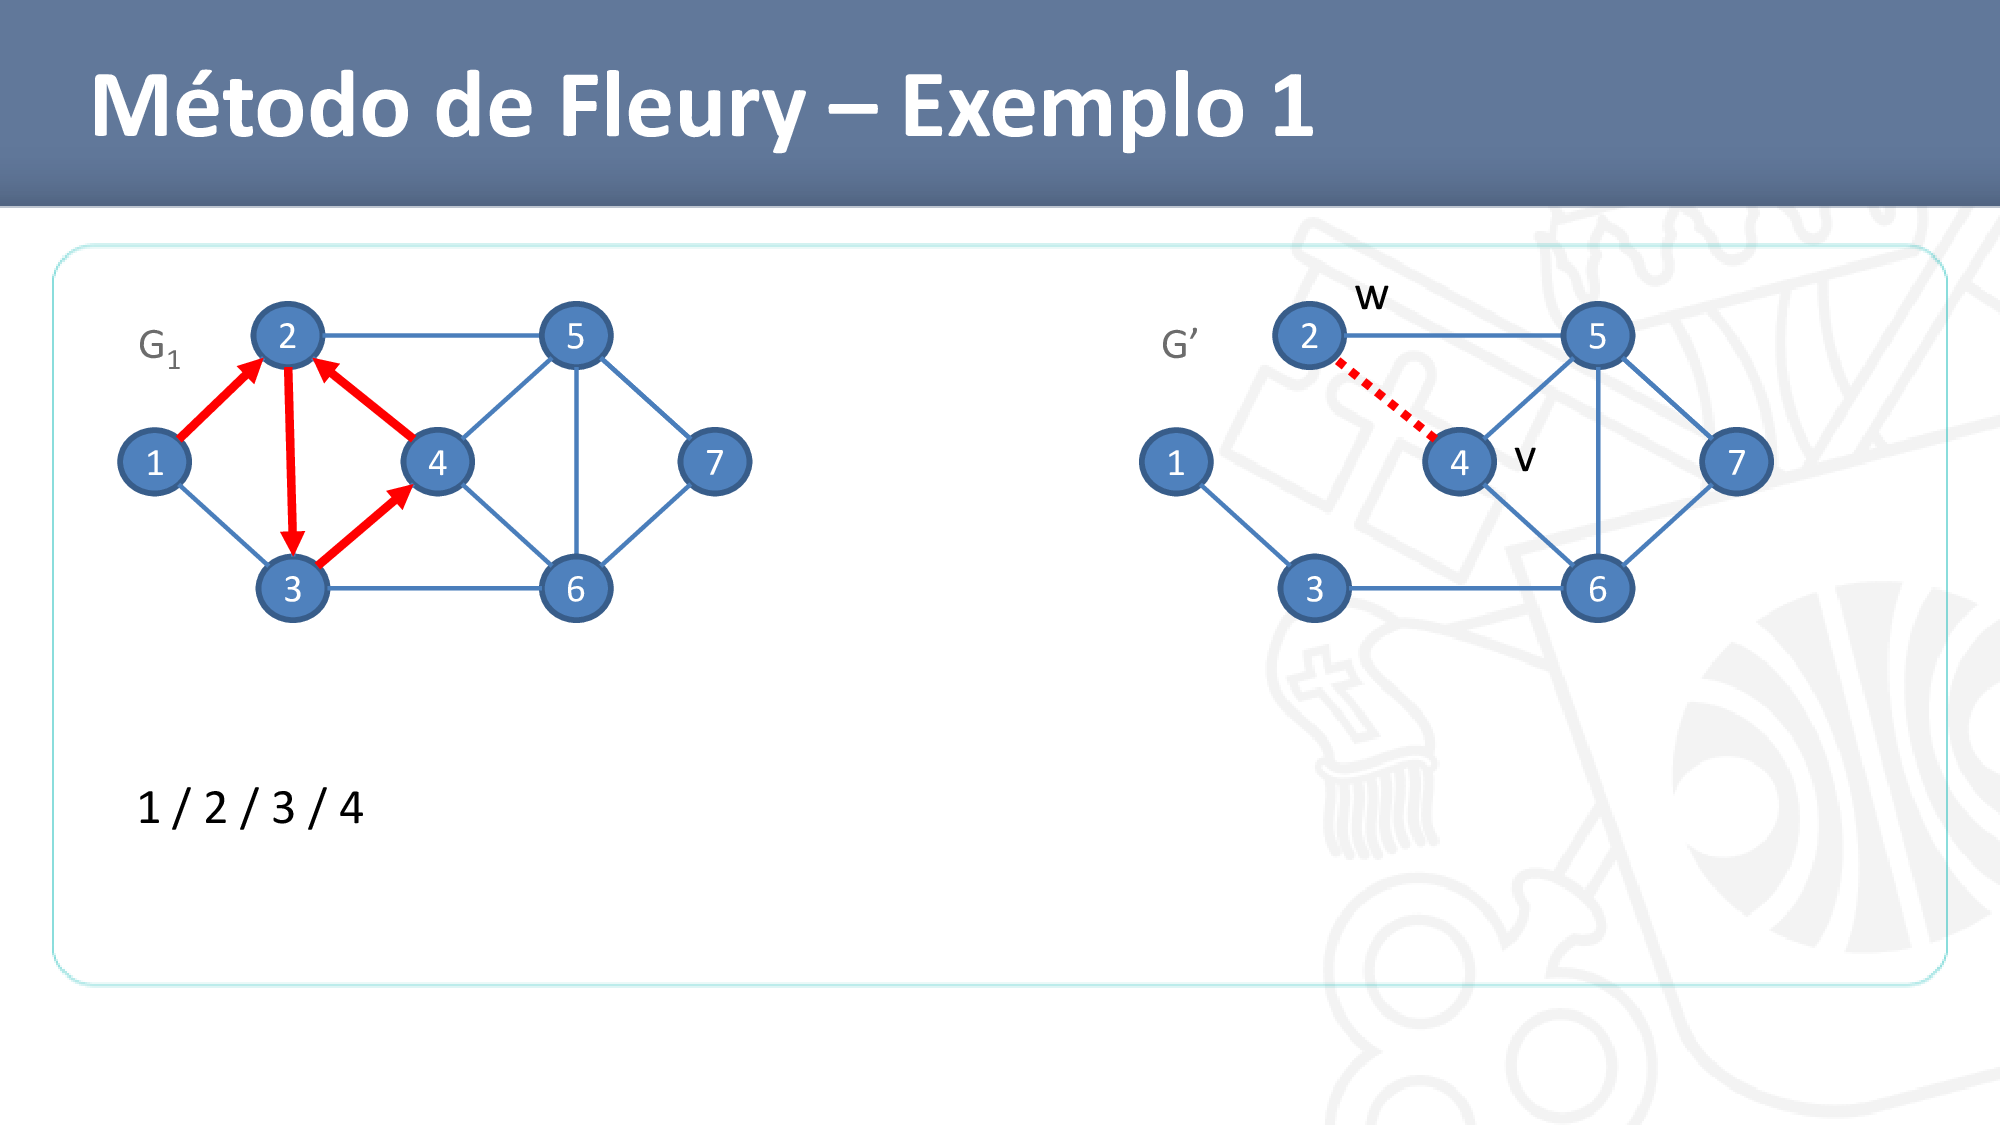
\includegraphics[width=\textwidth]{imagem/graficos/1a1455b7b9174768d1c6a0d41673e79dHTztESkzBtQzsXWu-32.png}
	\end{subfigure}
\end{figure}
\begin{figure}[htbp]
    \begin{subfigure}{.4\textwidth}
		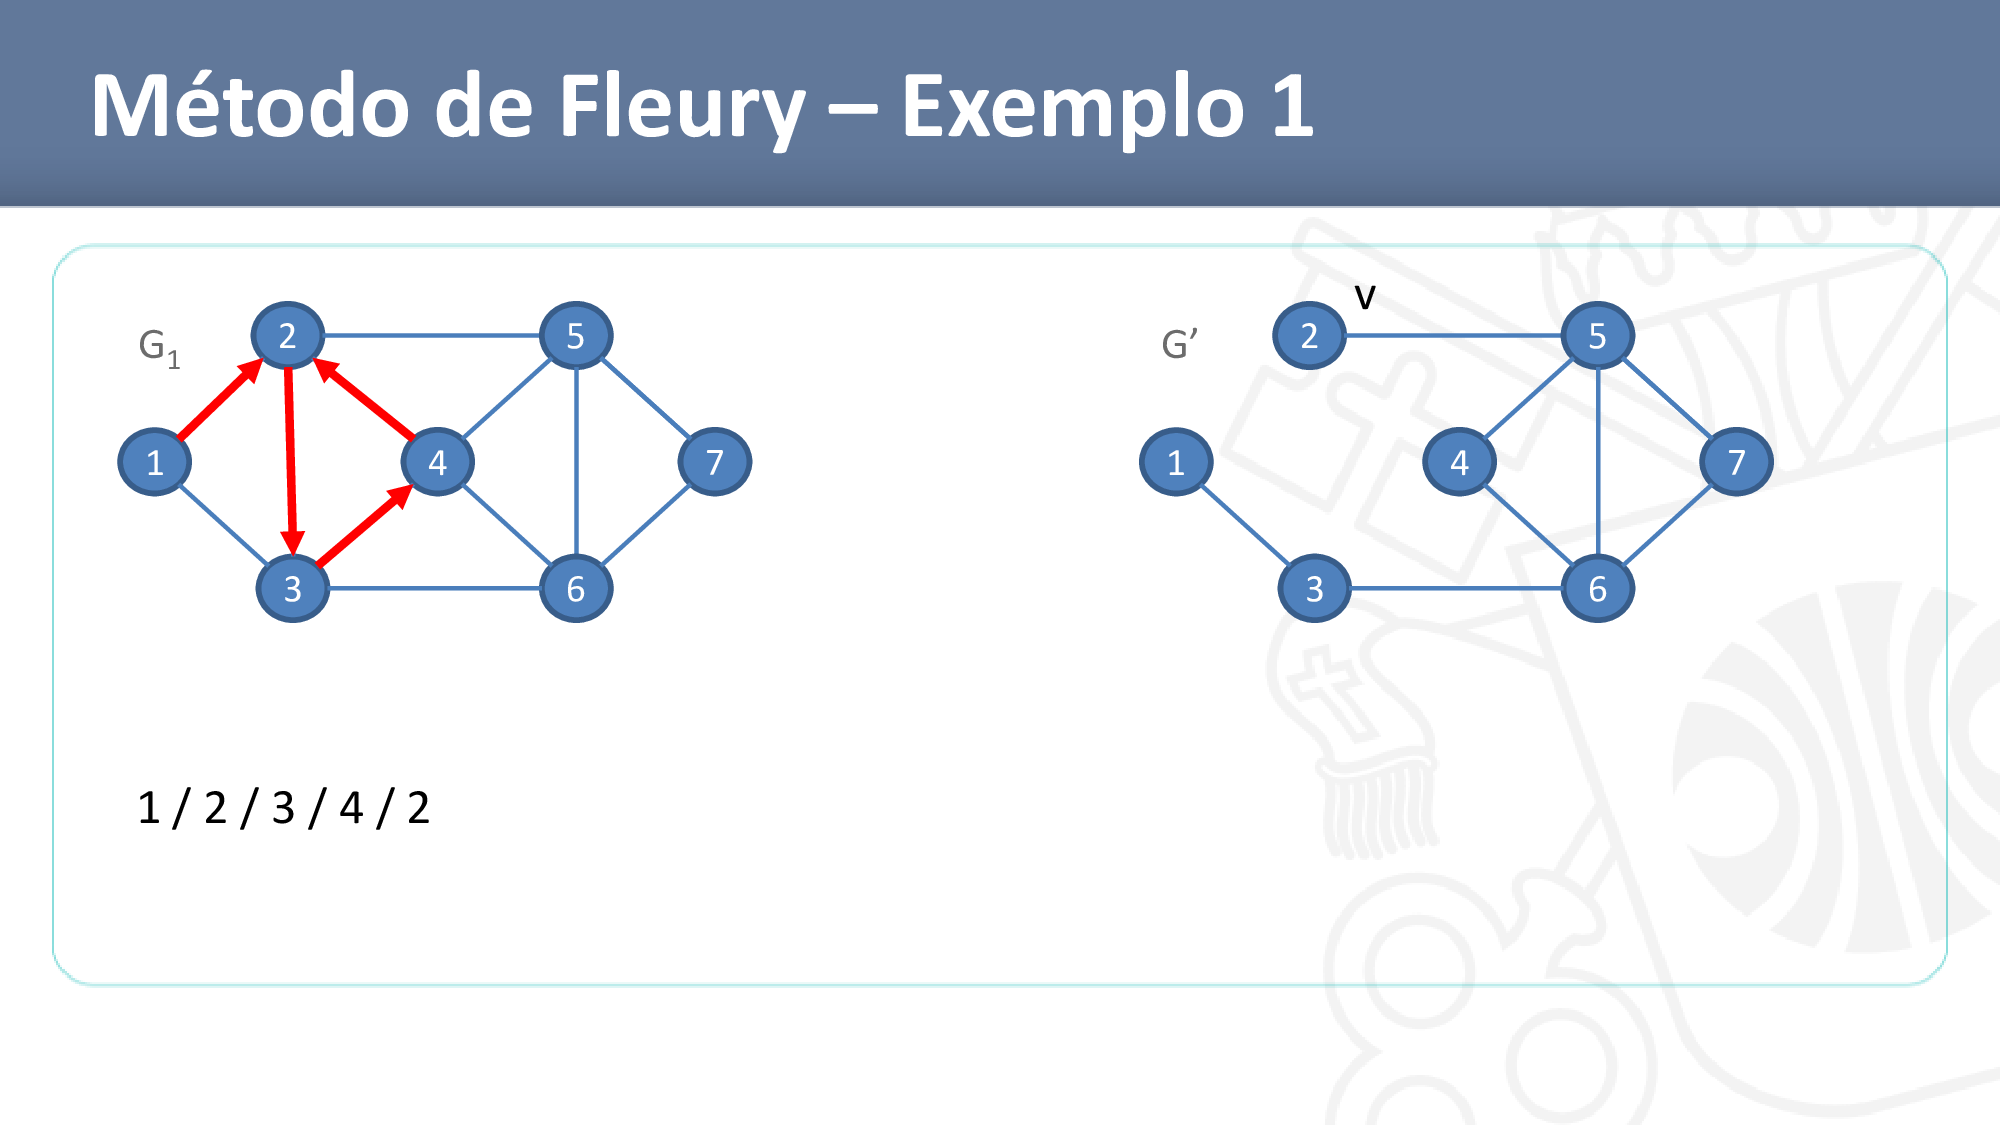
\includegraphics[width=\textwidth]{imagem/graficos/1a1455b7b9174768d1c6a0d41673e79dHTztESkzBtQzsXWu-33.png}
	\end{subfigure}
    \begin{subfigure}{.4\textwidth}
		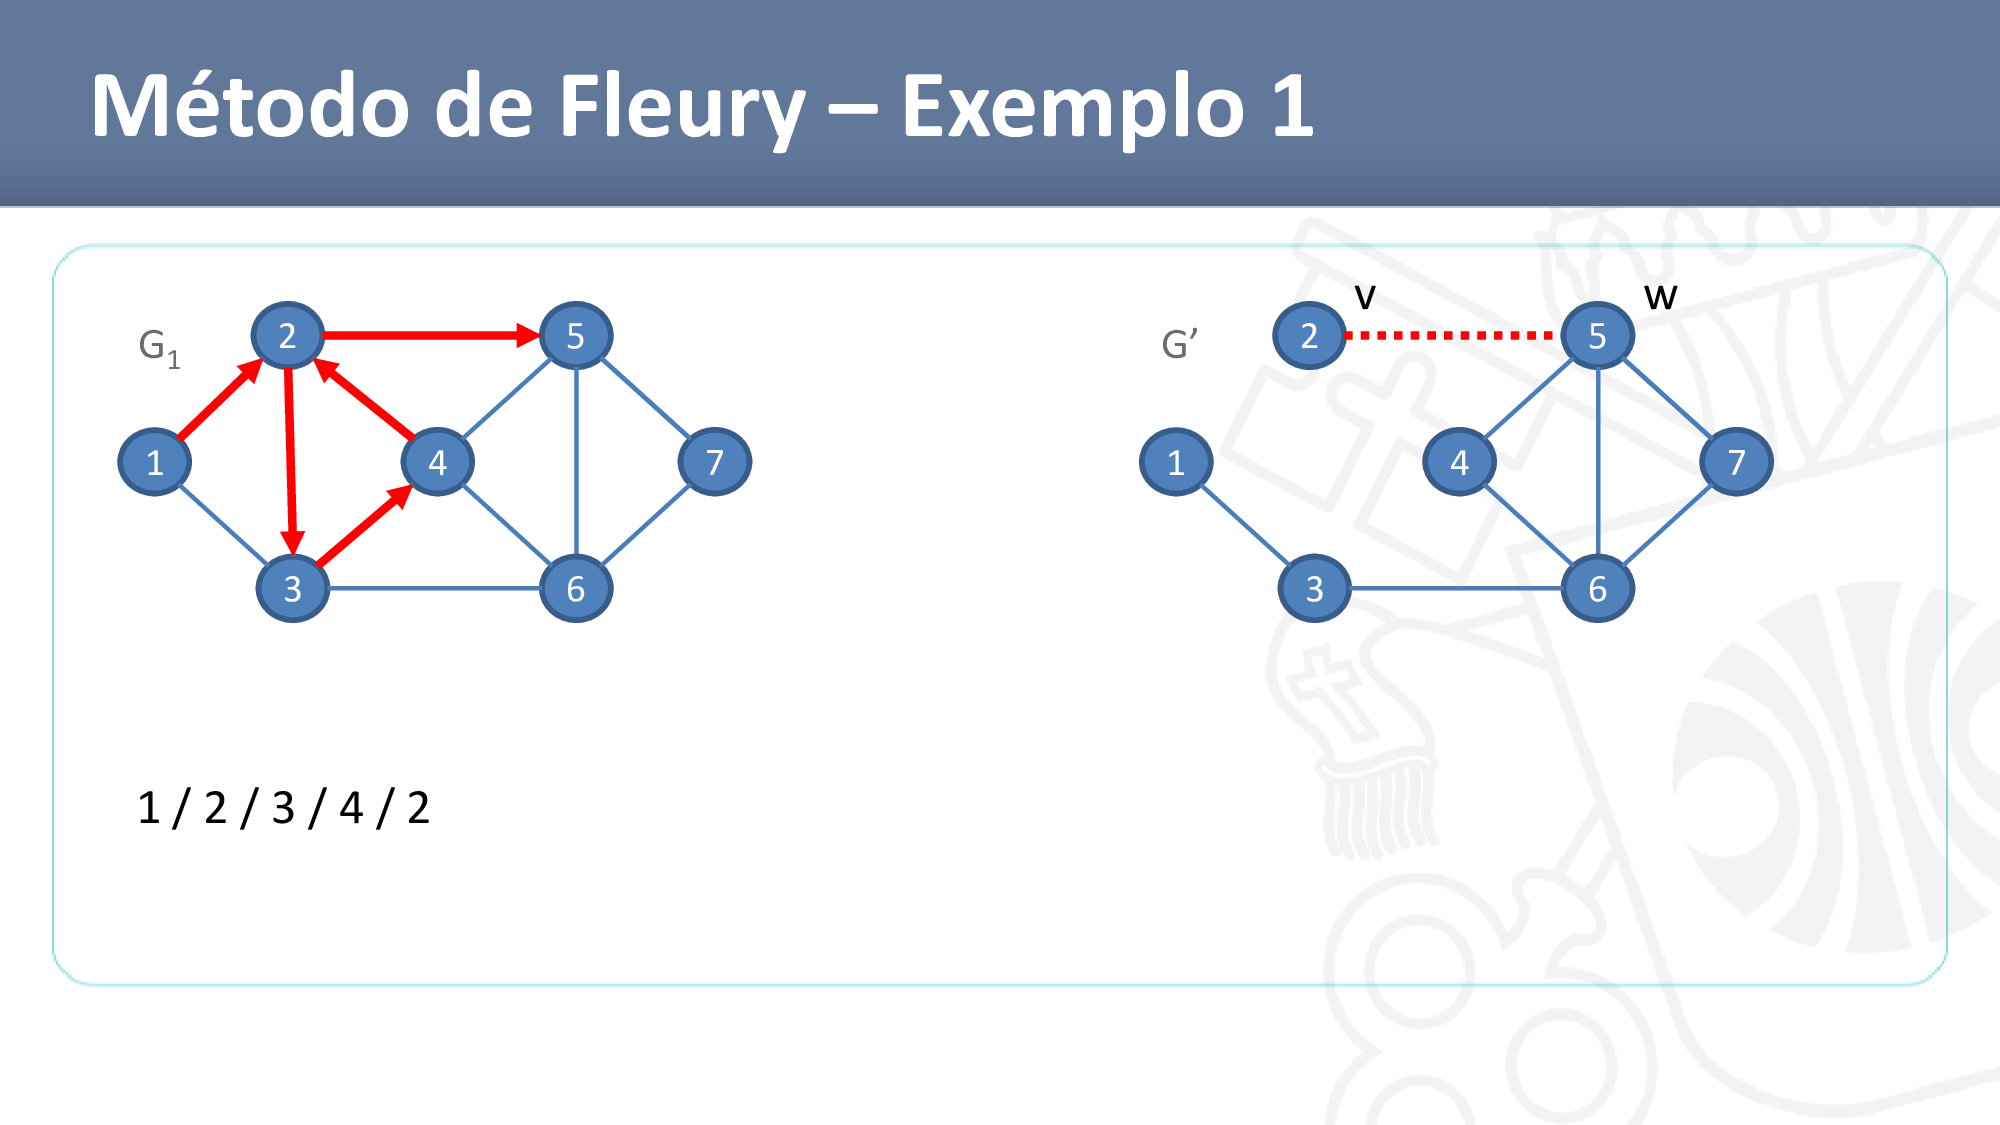
\includegraphics[width=\textwidth]{imagem/graficos/1a1455b7b9174768d1c6a0d41673e79dHTztESkzBtQzsXWu-34.png}
	\end{subfigure}
\end{figure}
\begin{figure}[htbp]
    \begin{subfigure}{.4\textwidth}
		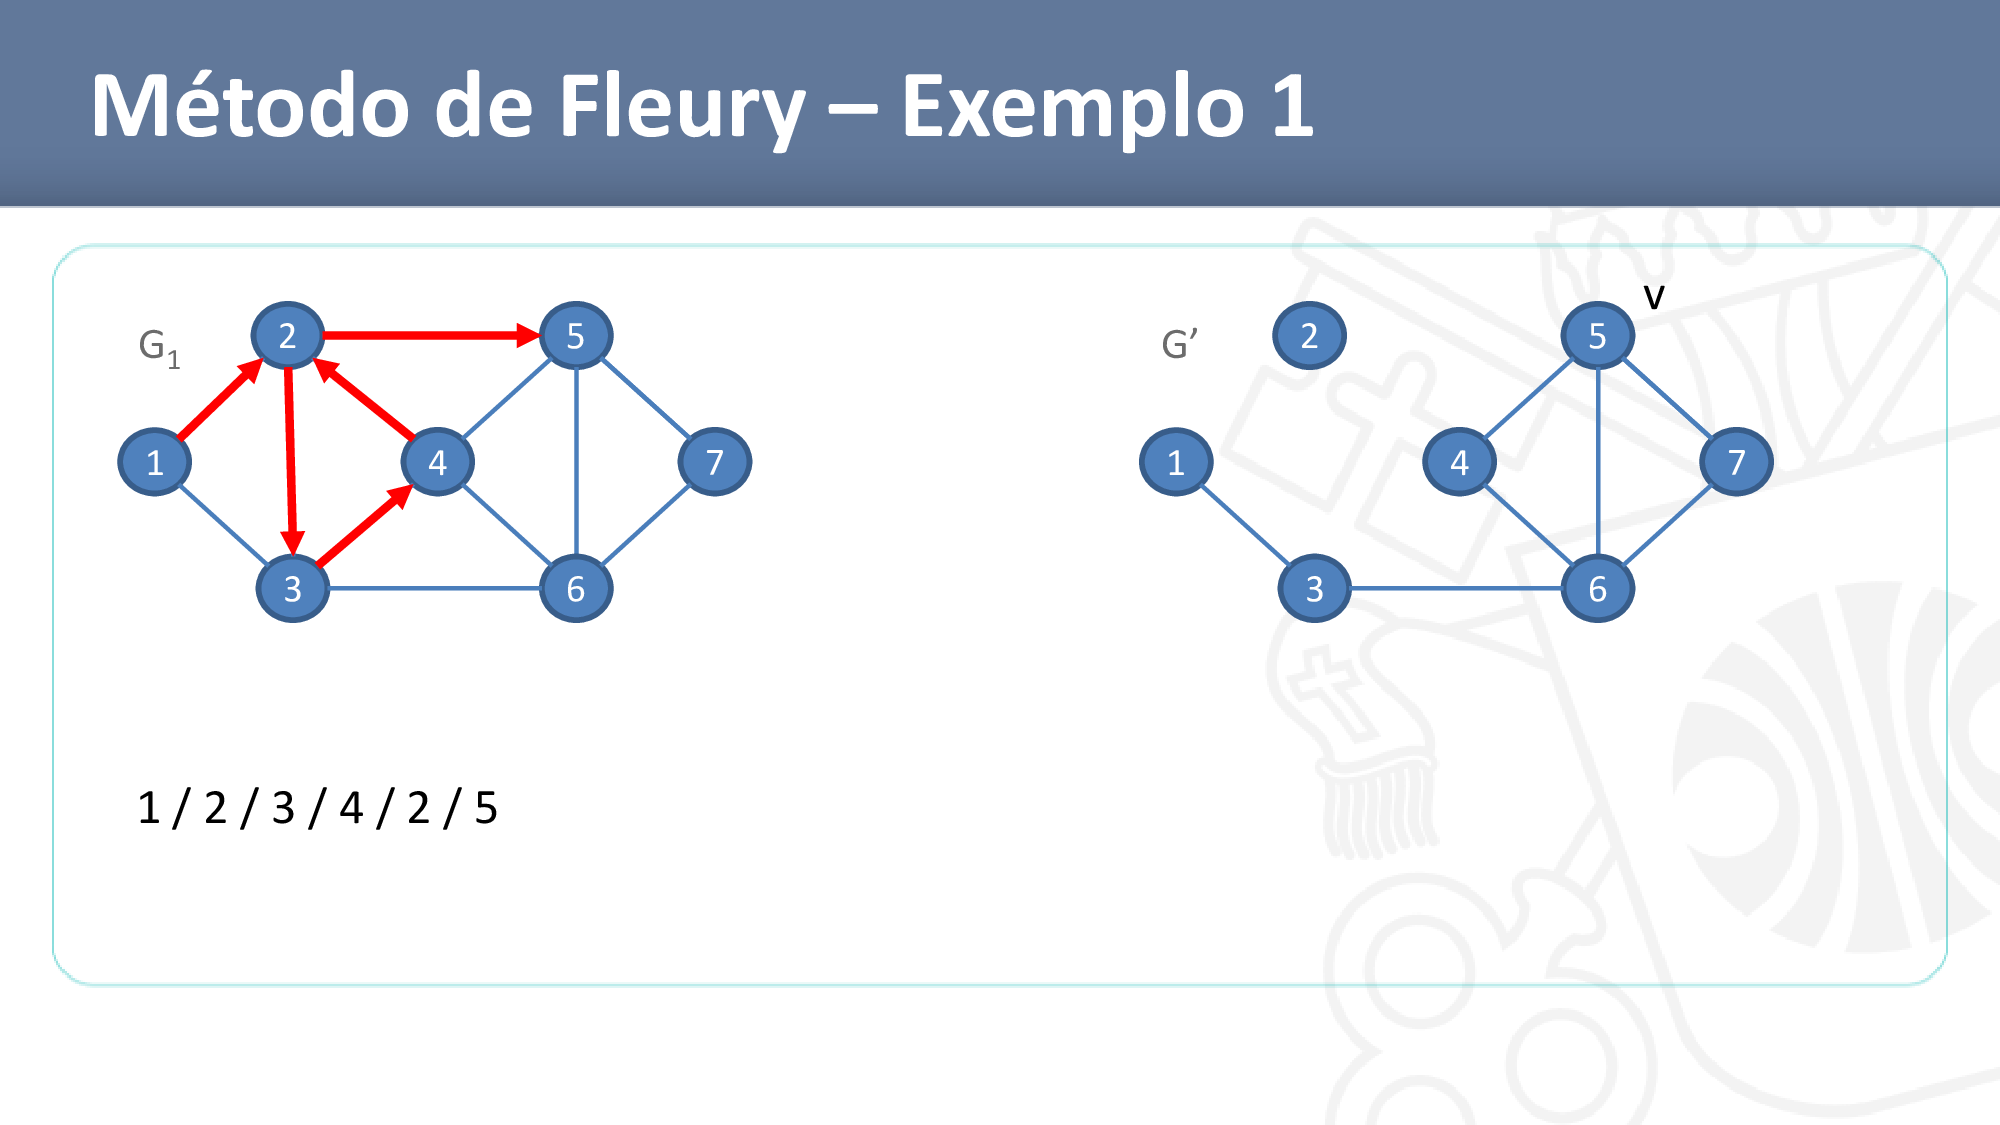
\includegraphics[width=\textwidth]{imagem/graficos/1a1455b7b9174768d1c6a0d41673e79dHTztESkzBtQzsXWu-35.png}
	\end{subfigure}
    \begin{subfigure}{.4\textwidth}
		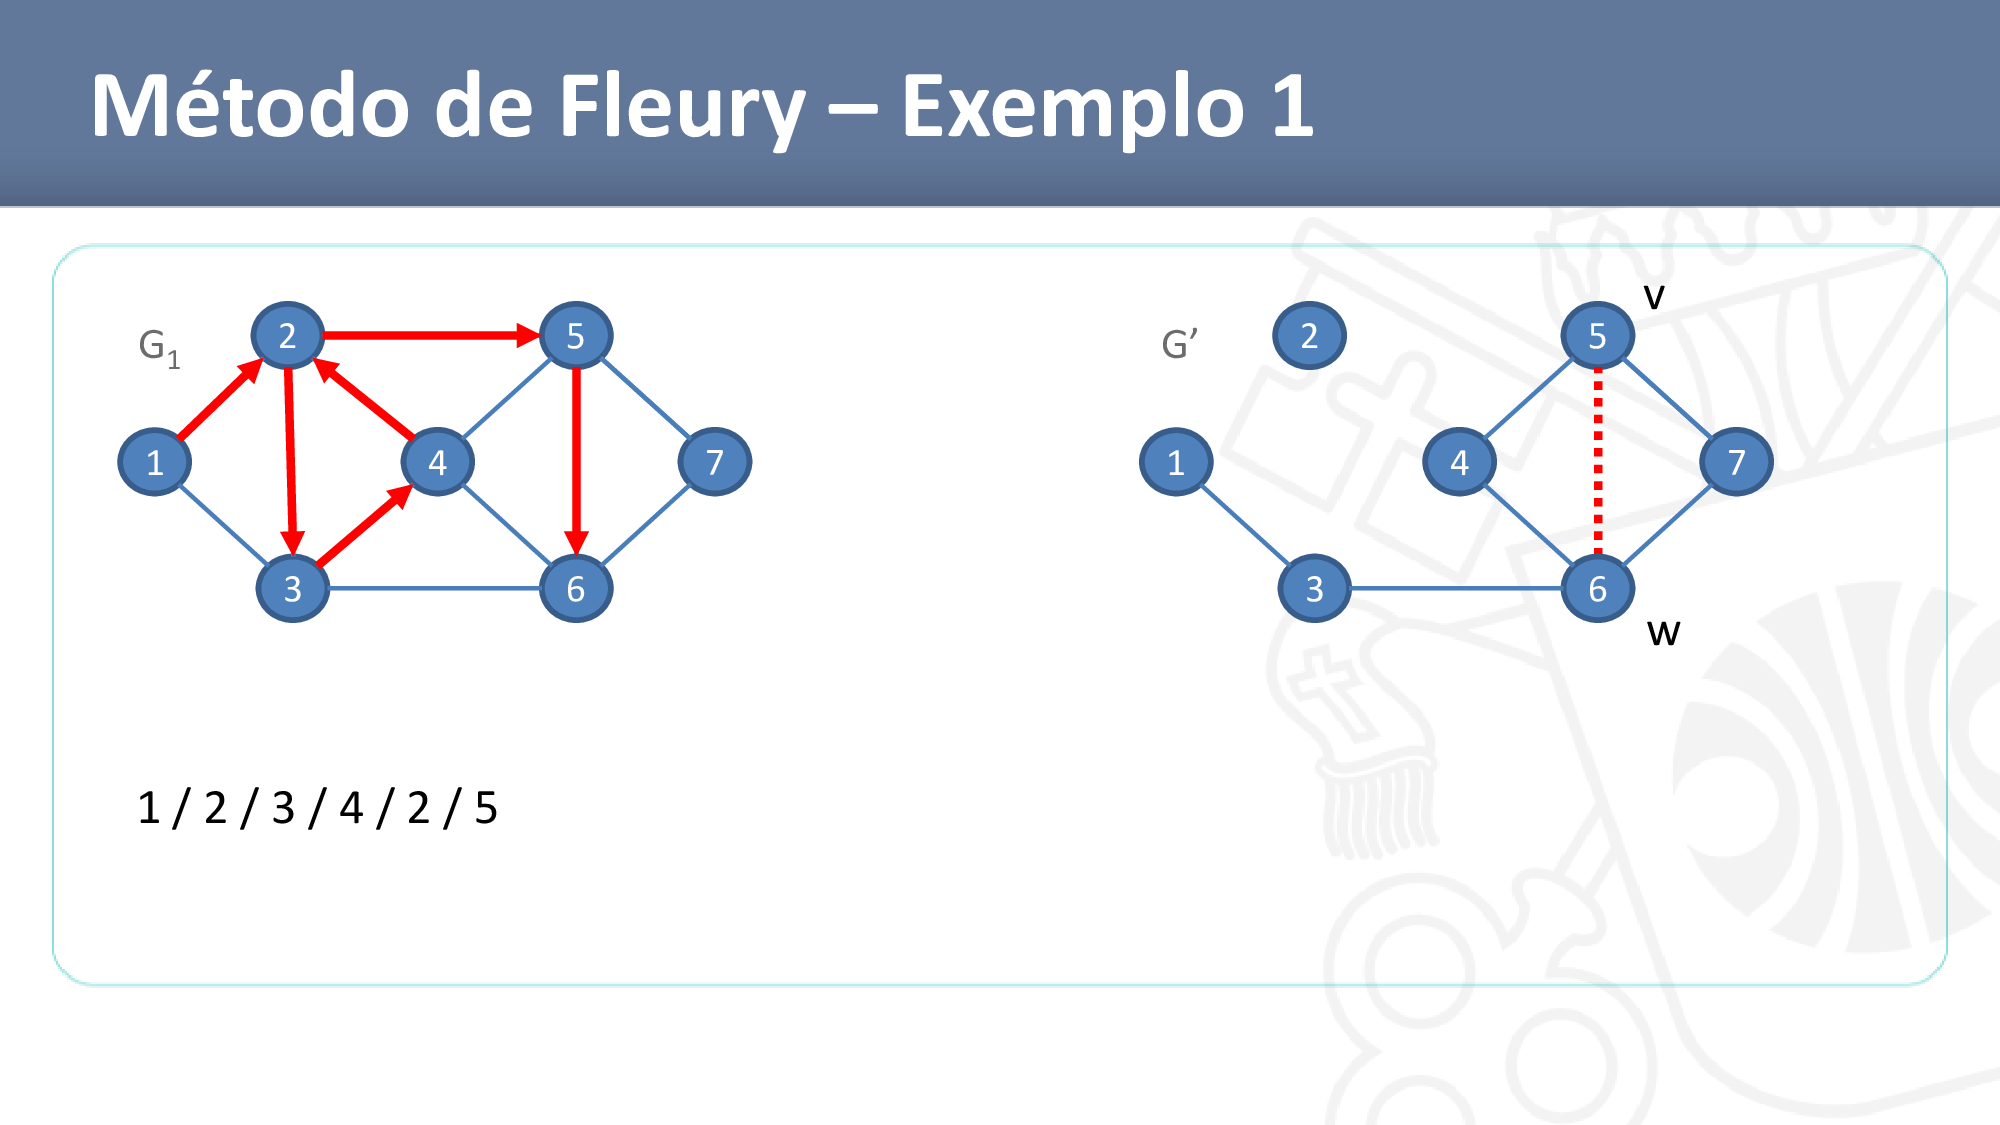
\includegraphics[width=\textwidth]{imagem/graficos/1a1455b7b9174768d1c6a0d41673e79dHTztESkzBtQzsXWu-36.png}
	\end{subfigure}
\end{figure}
\begin{figure}[htbp]
    \begin{subfigure}{.4\textwidth}
		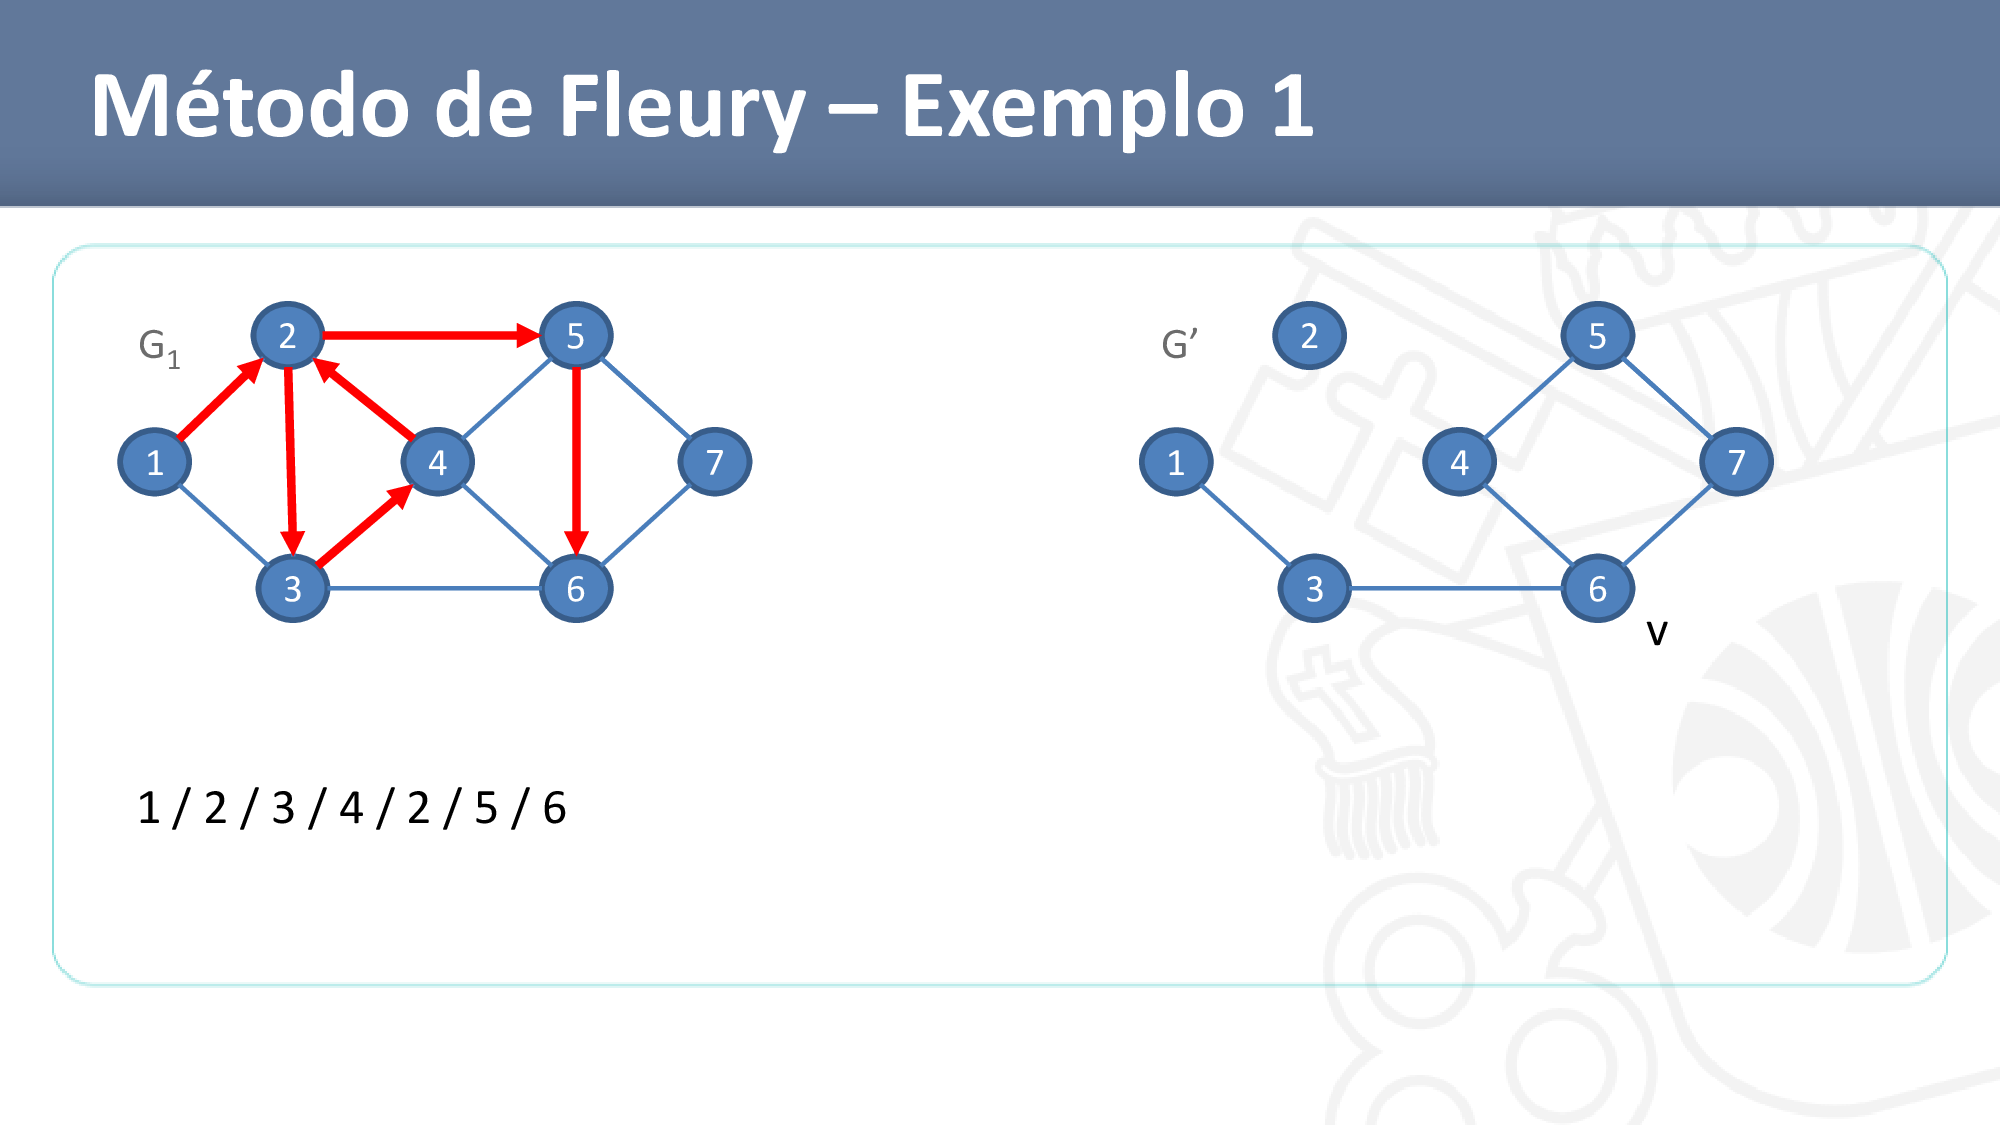
\includegraphics[width=\textwidth]{imagem/graficos/1a1455b7b9174768d1c6a0d41673e79dHTztESkzBtQzsXWu-37.png}
	\end{subfigure}
    \begin{subfigure}{.4\textwidth}
		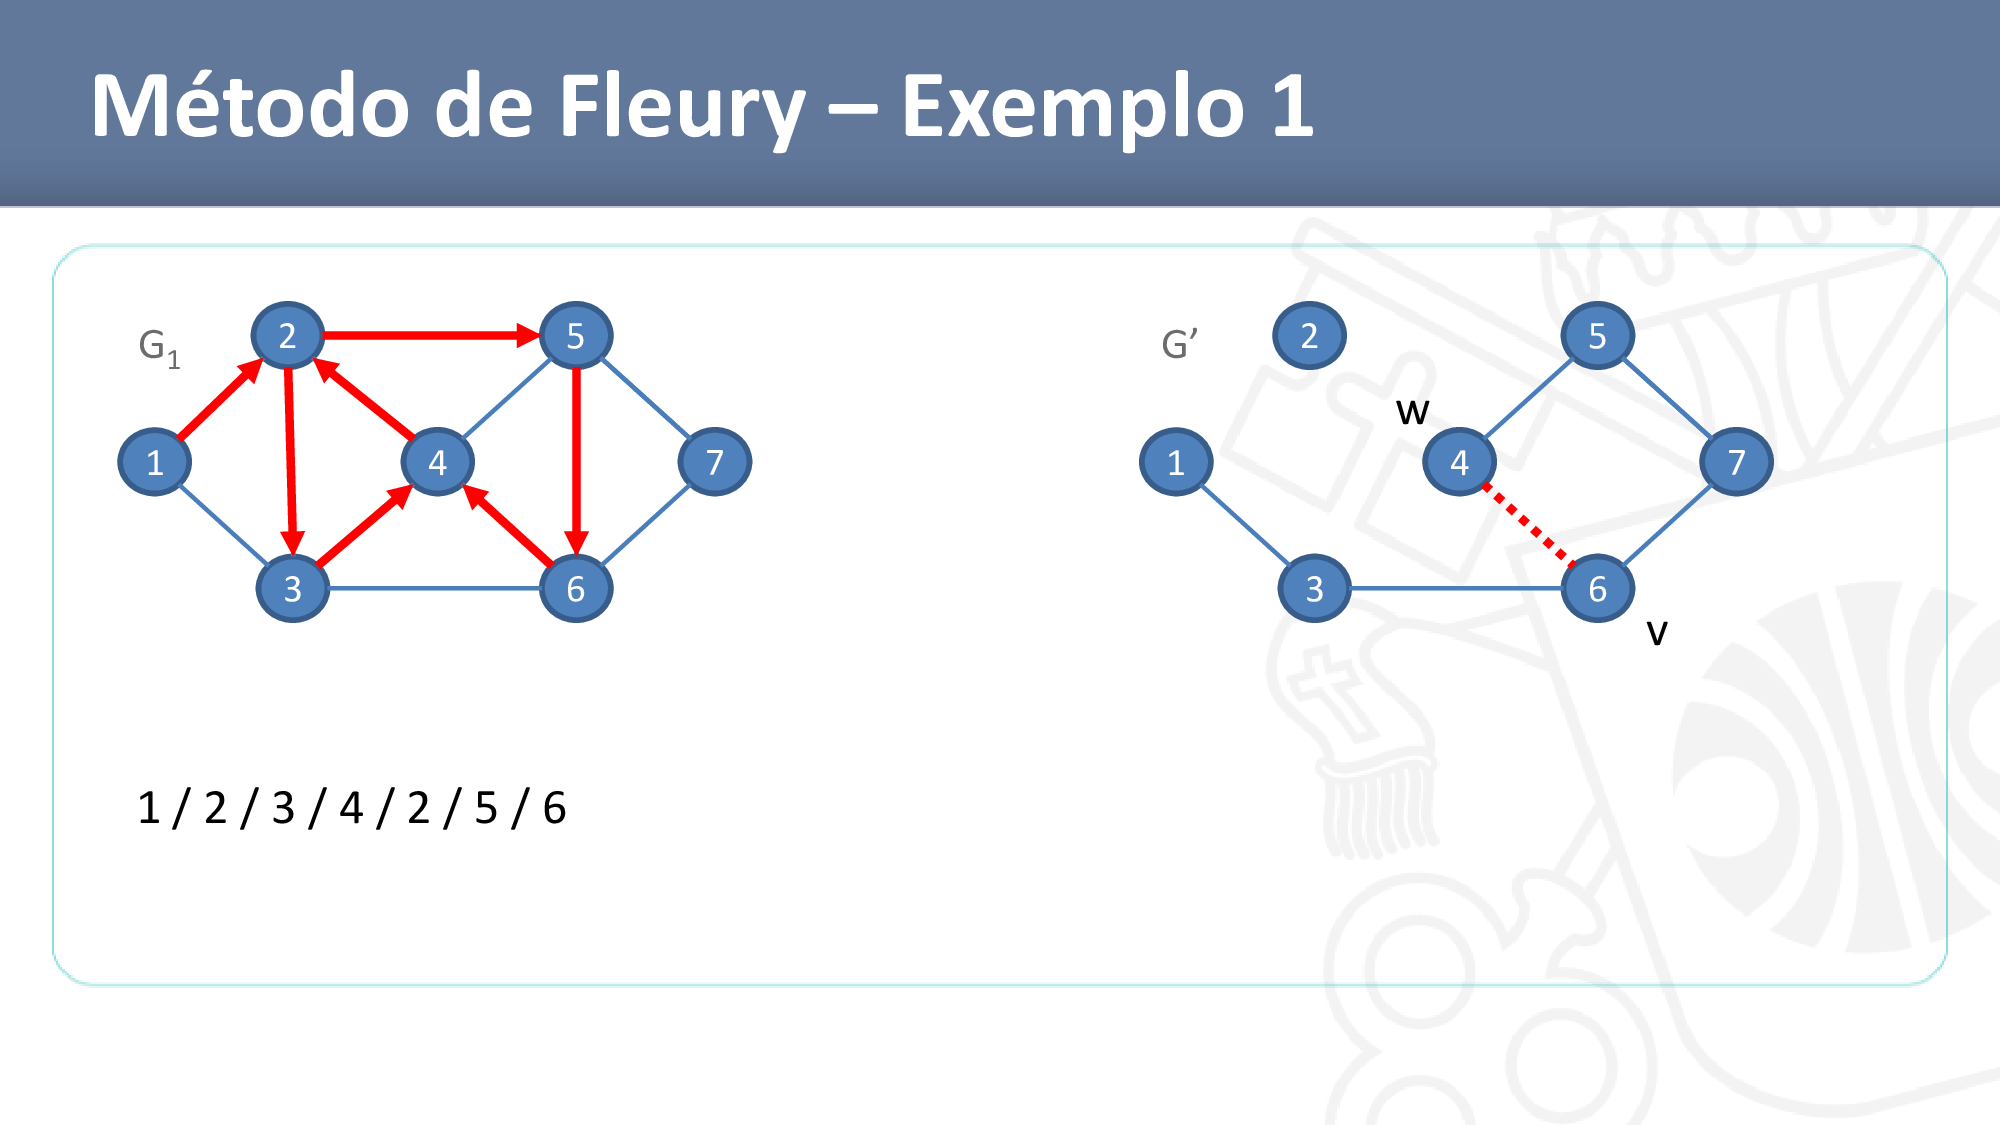
\includegraphics[width=\textwidth]{imagem/graficos/1a1455b7b9174768d1c6a0d41673e79dHTztESkzBtQzsXWu-38.png}
	\end{subfigure}
\end{figure}
\begin{figure}[htbp]  
    \begin{subfigure}{.4\textwidth}
		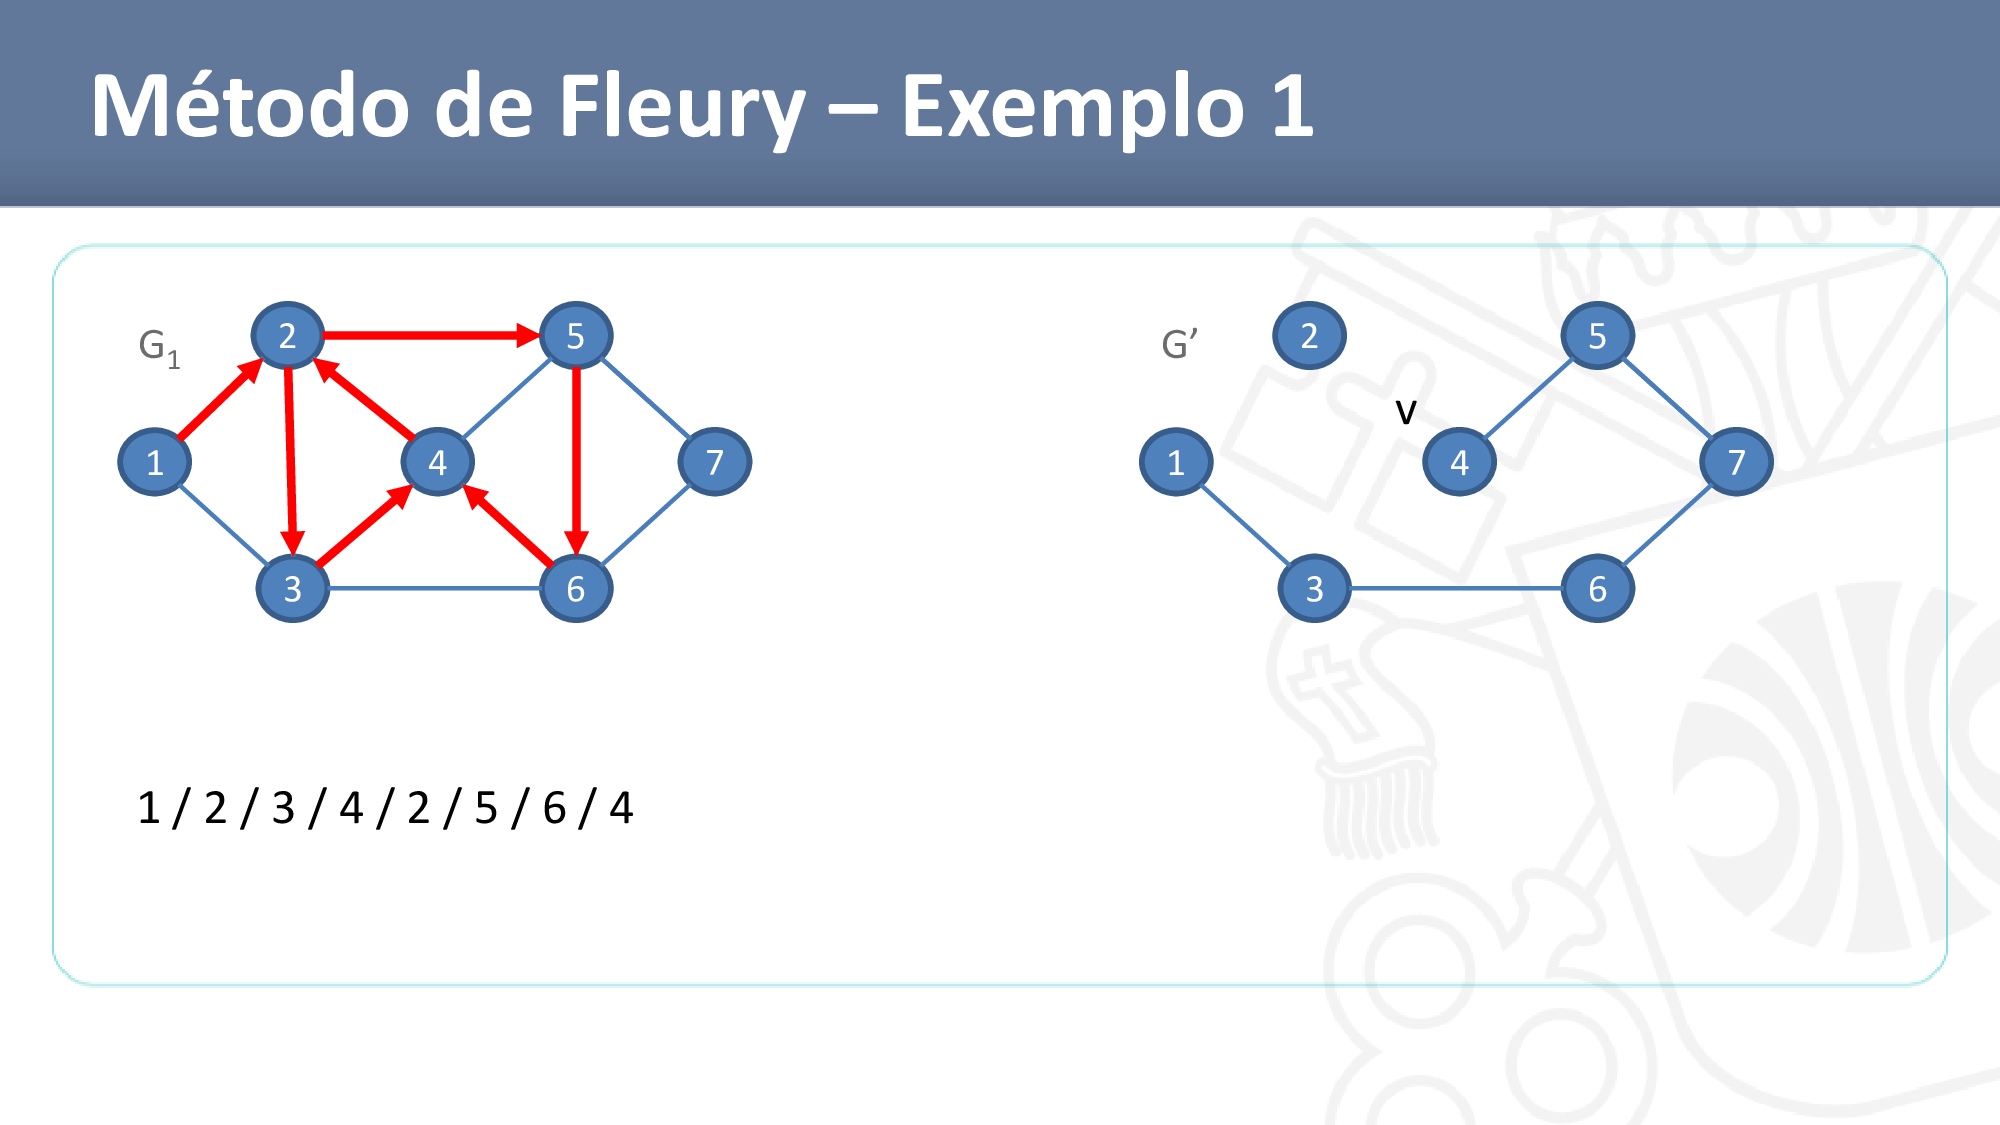
\includegraphics[width=\textwidth]{imagem/graficos/1a1455b7b9174768d1c6a0d41673e79dHTztESkzBtQzsXWu-39.png}
	\end{subfigure}
    \begin{subfigure}{.4\textwidth}
		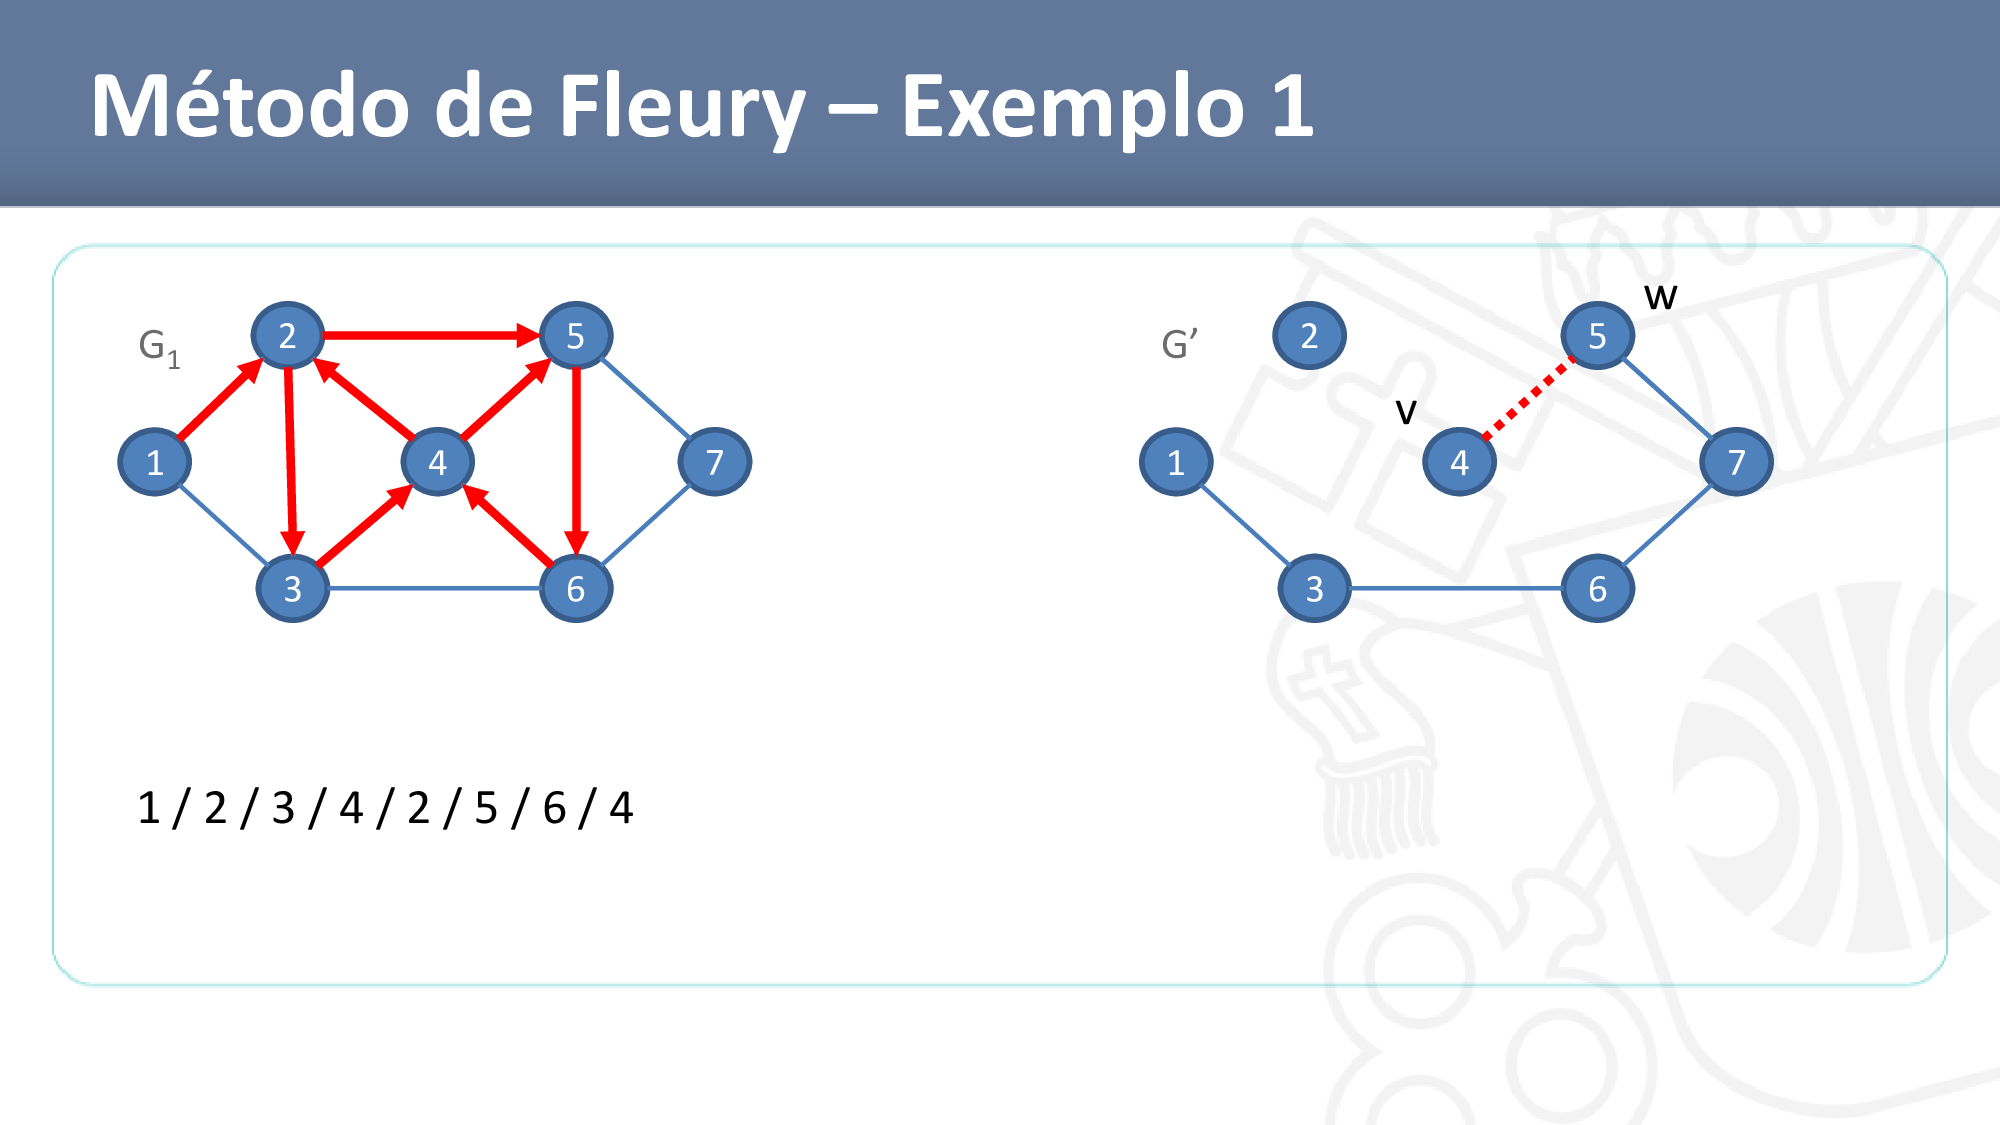
\includegraphics[width=\textwidth]{imagem/graficos/1a1455b7b9174768d1c6a0d41673e79dHTztESkzBtQzsXWu-40.png}
	\end{subfigure}
\end{figure}  
\begin{figure}[htbp]  
    \begin{subfigure}{.4\textwidth}
		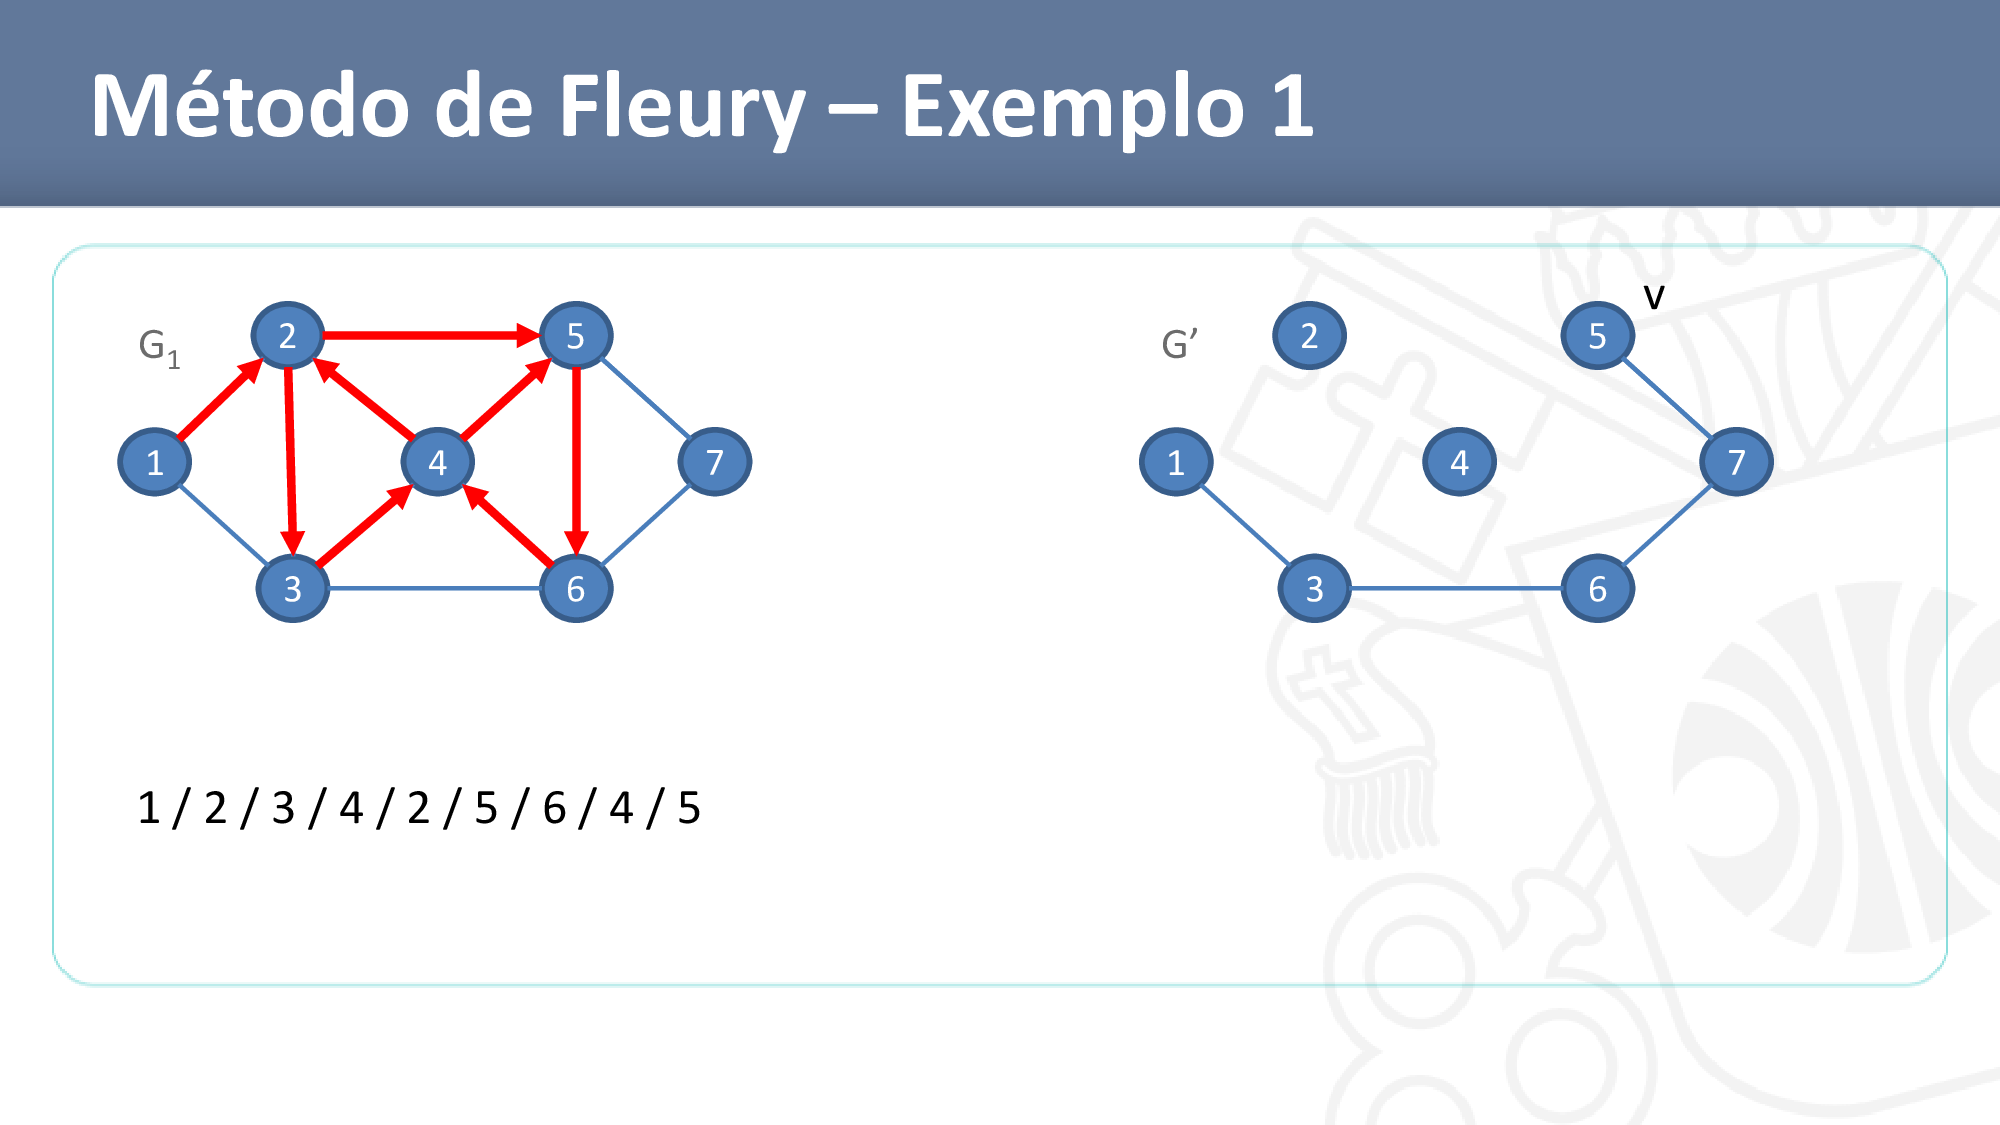
\includegraphics[width=\textwidth]{imagem/graficos/1a1455b7b9174768d1c6a0d41673e79dHTztESkzBtQzsXWu-41.png}
	\end{subfigure}
    \begin{subfigure}{.4\textwidth}
		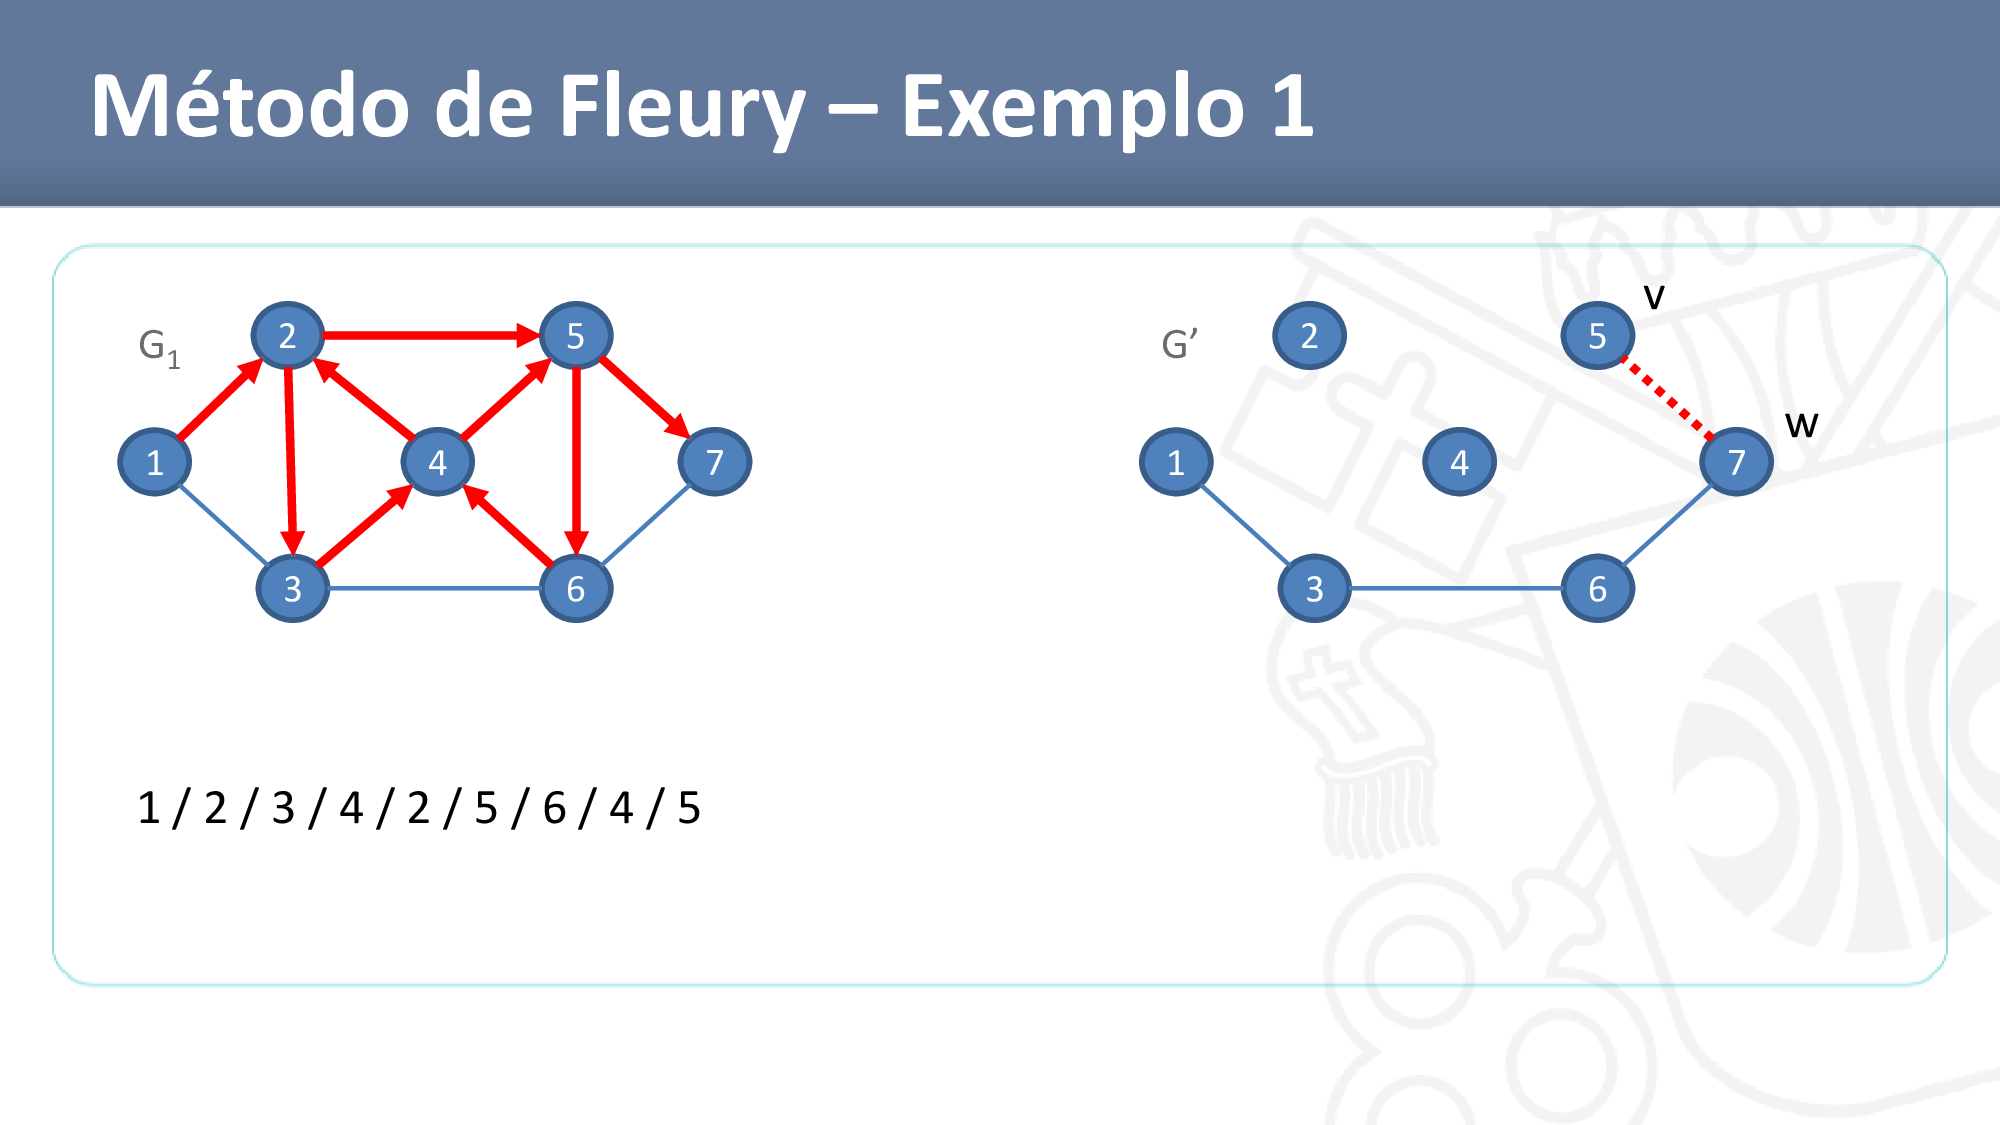
\includegraphics[width=\textwidth]{imagem/graficos/1a1455b7b9174768d1c6a0d41673e79dHTztESkzBtQzsXWu-42.png}
	\end{subfigure}
\end{figure}    
\begin{figure}[htbp]  
    \begin{subfigure}{.4\textwidth}
		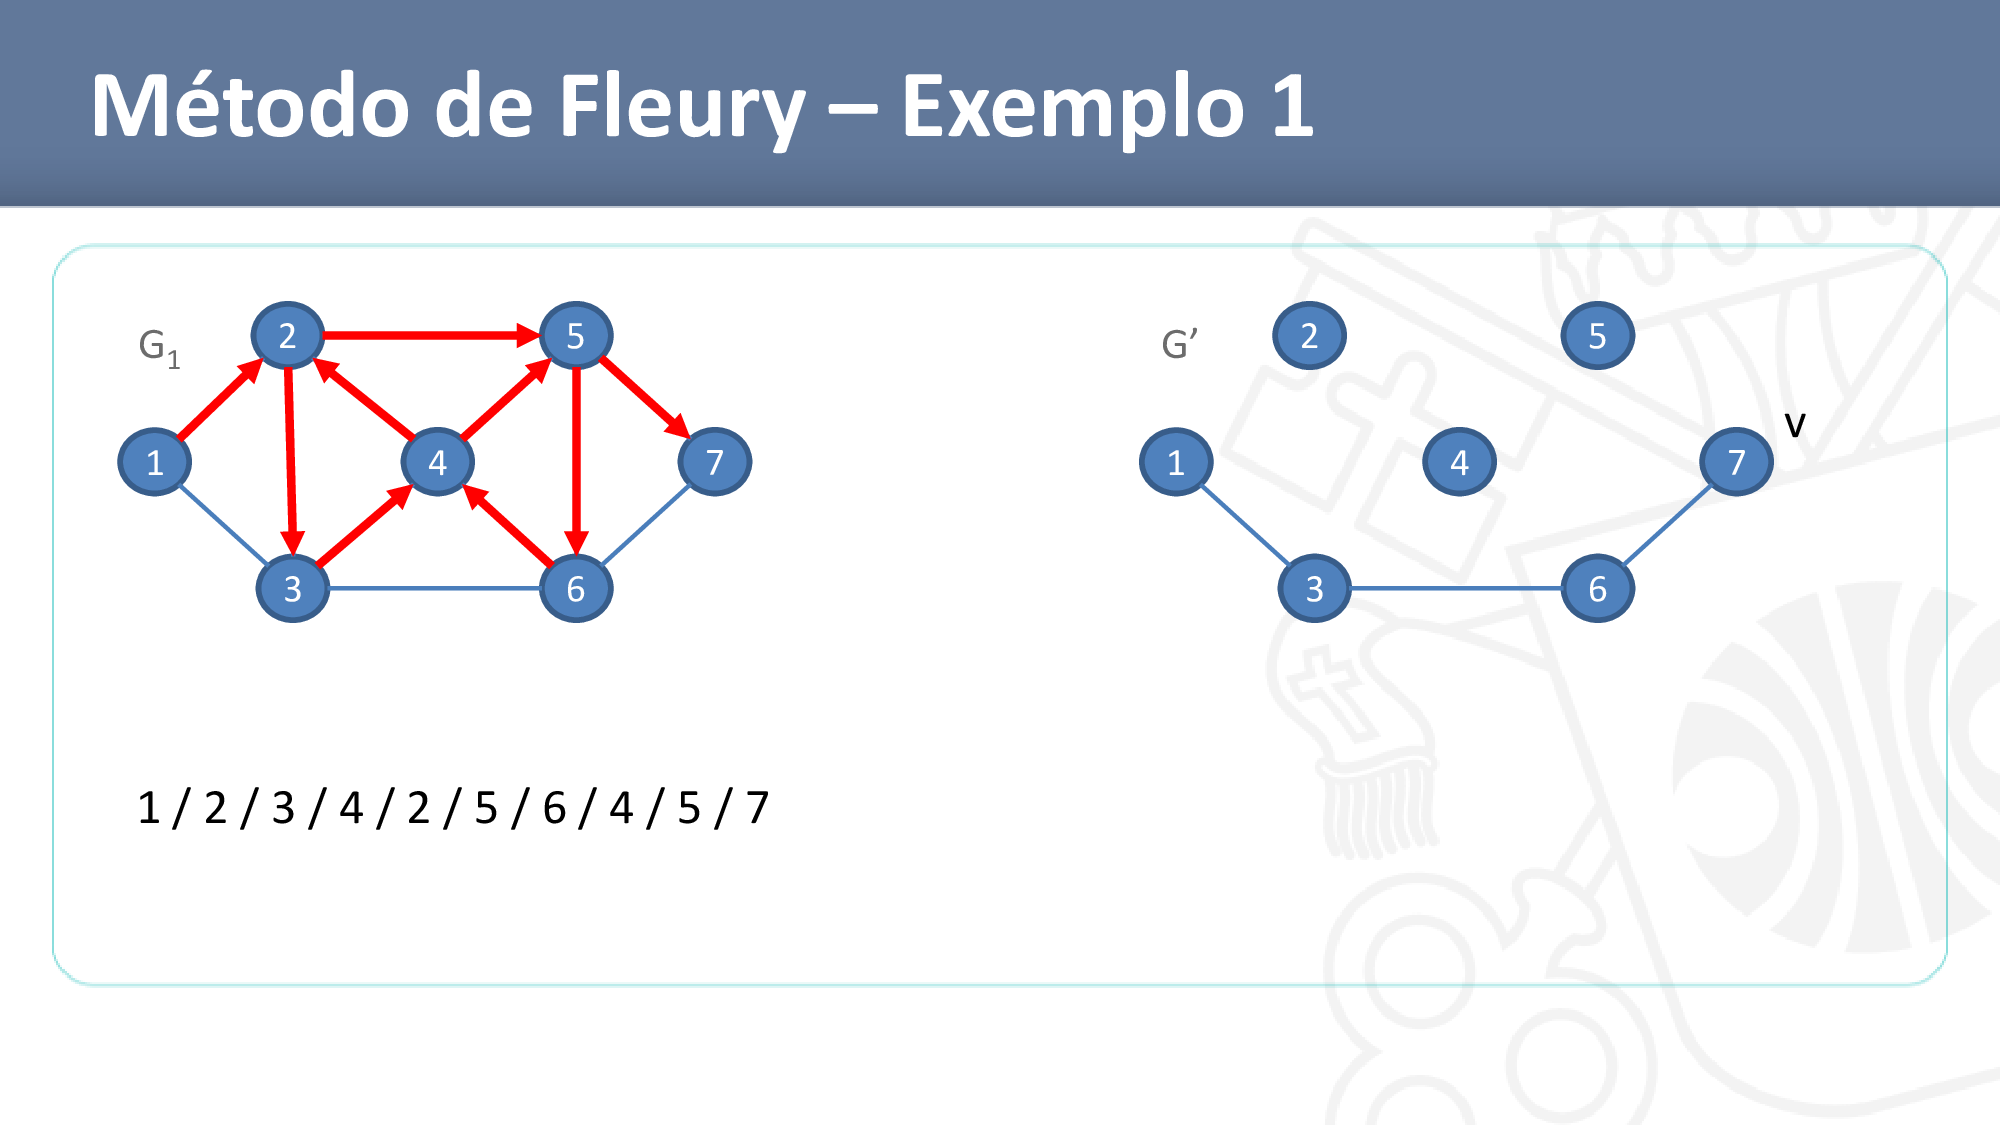
\includegraphics[width=\textwidth]{imagem/graficos/1a1455b7b9174768d1c6a0d41673e79dHTztESkzBtQzsXWu-43.png}
	\end{subfigure}
    \begin{subfigure}{.4\textwidth}
		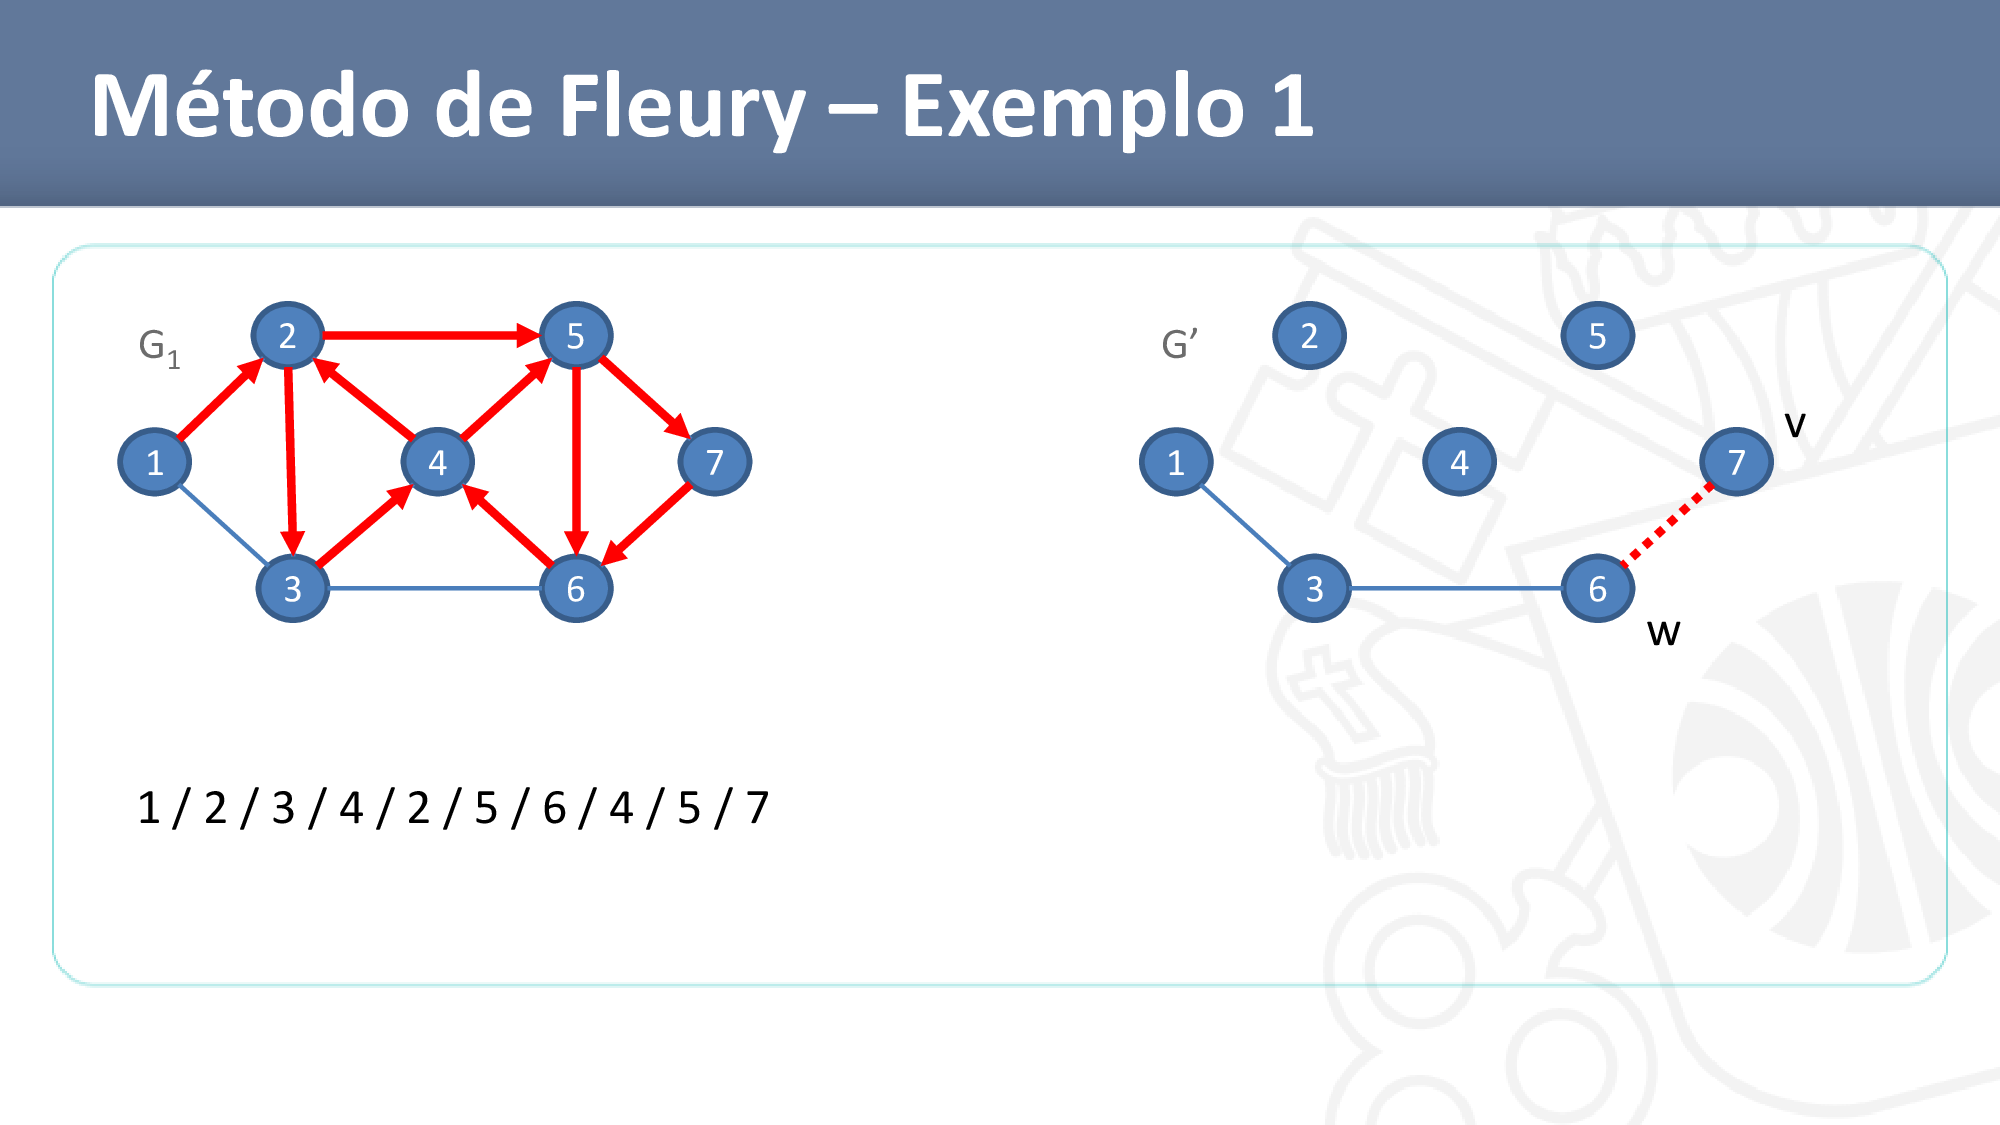
\includegraphics[width=\textwidth]{imagem/graficos/1a1455b7b9174768d1c6a0d41673e79dHTztESkzBtQzsXWu-44.png}
	\end{subfigure}
\end{figure}    
\begin{figure}[htbp]  
    \begin{subfigure}{.4\textwidth}
		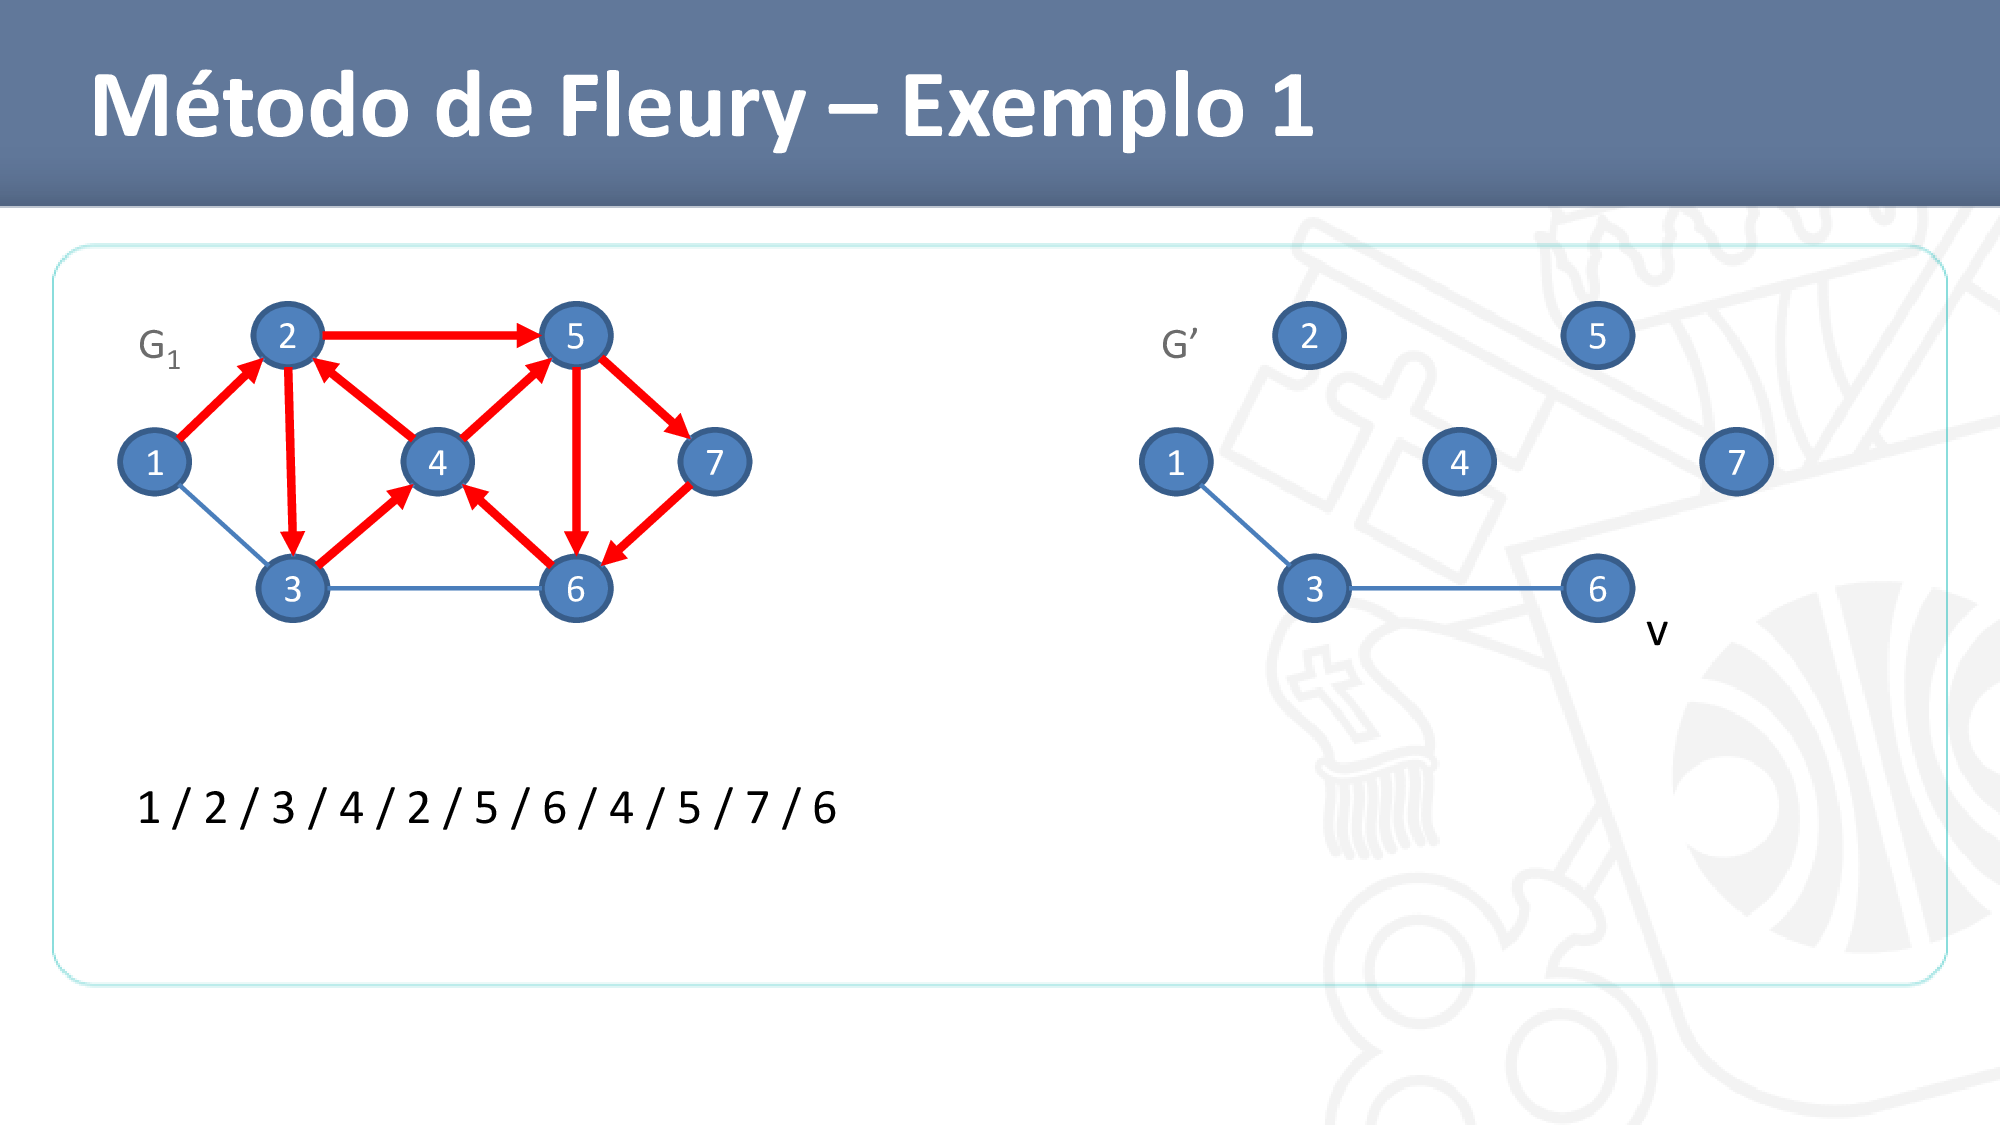
\includegraphics[width=\textwidth]{imagem/graficos/1a1455b7b9174768d1c6a0d41673e79dHTztESkzBtQzsXWu-45.png}
	\end{subfigure}
    \begin{subfigure}{.4\textwidth}
		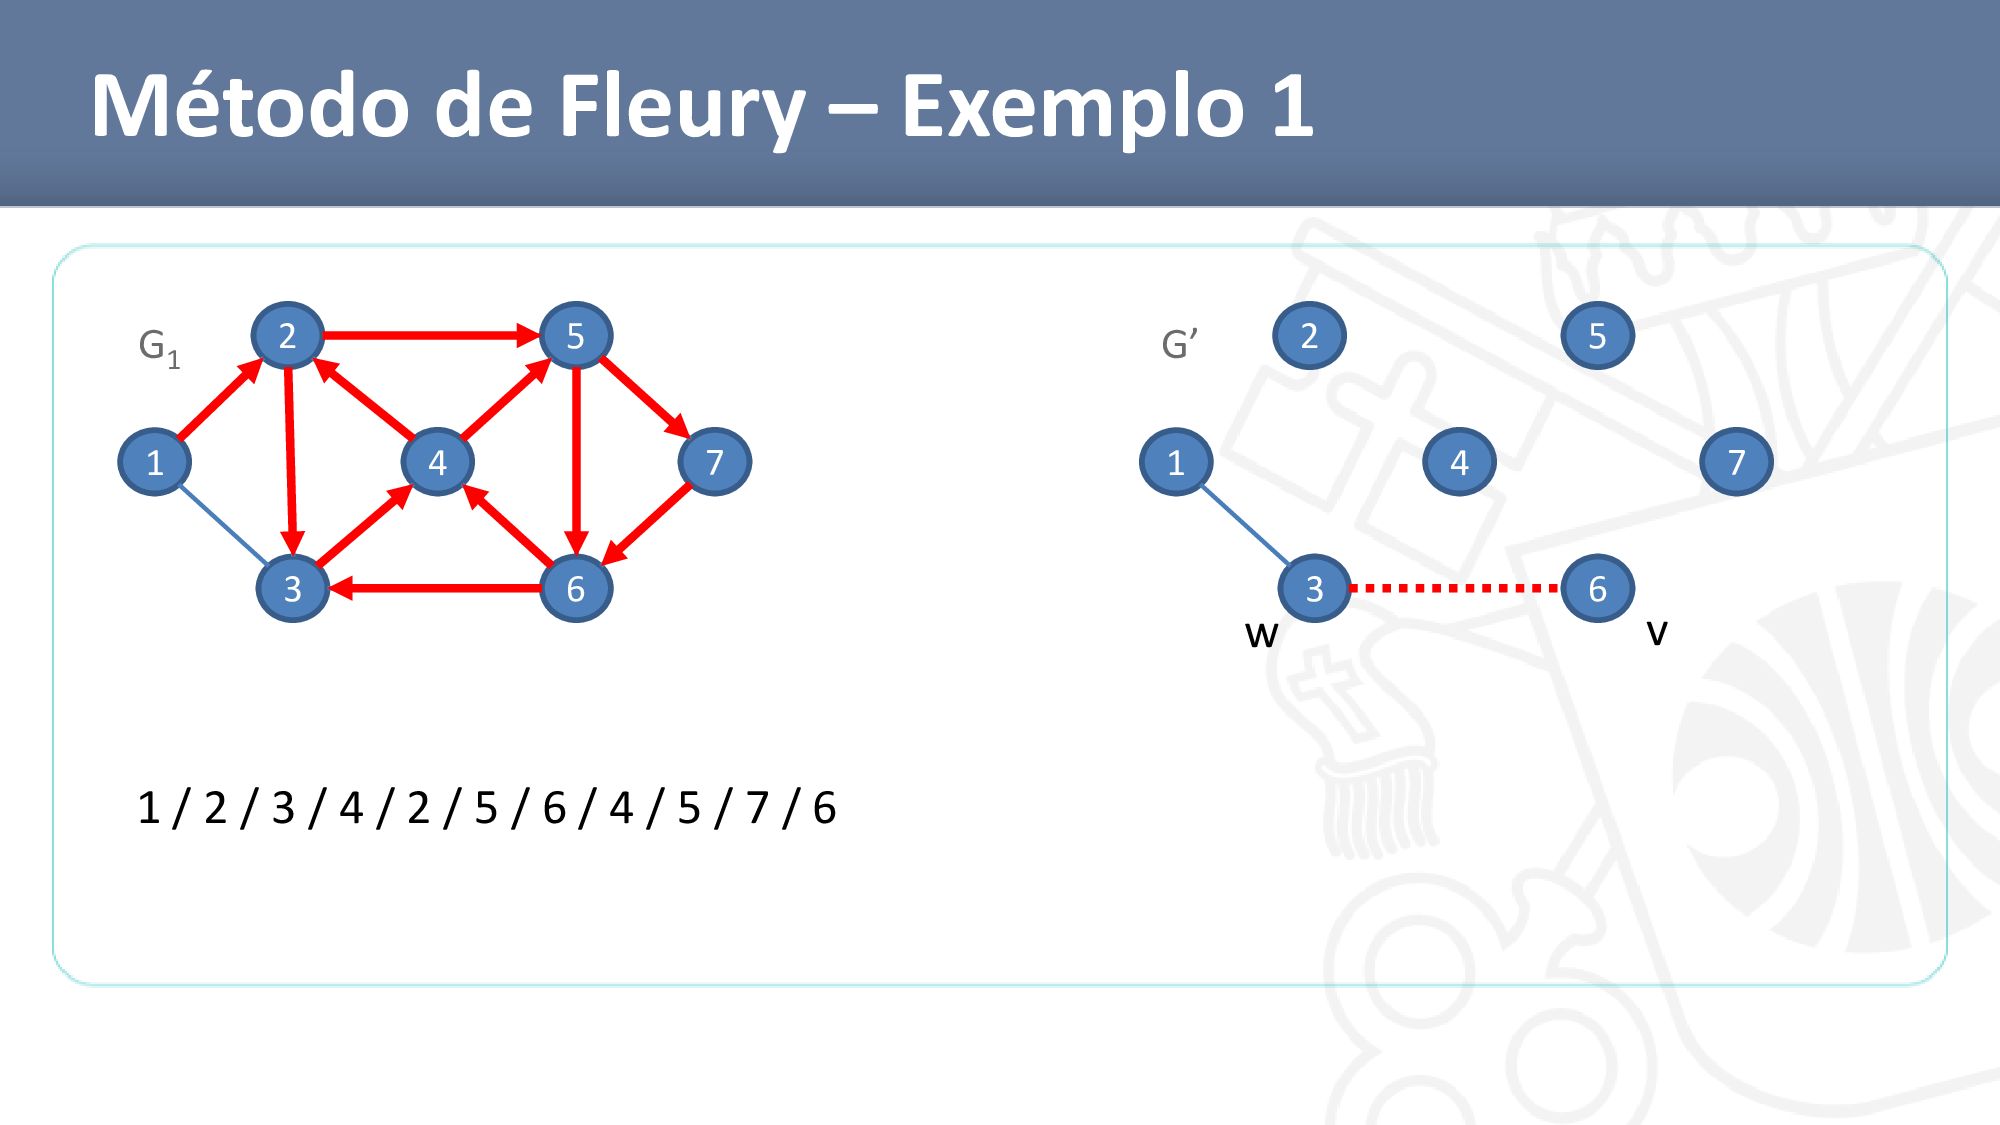
\includegraphics[width=\textwidth]{imagem/graficos/1a1455b7b9174768d1c6a0d41673e79dHTztESkzBtQzsXWu-46.png}
	\end{subfigure}
\end{figure}    
\begin{figure}[htbp]  
    \begin{subfigure}{.4\textwidth}
		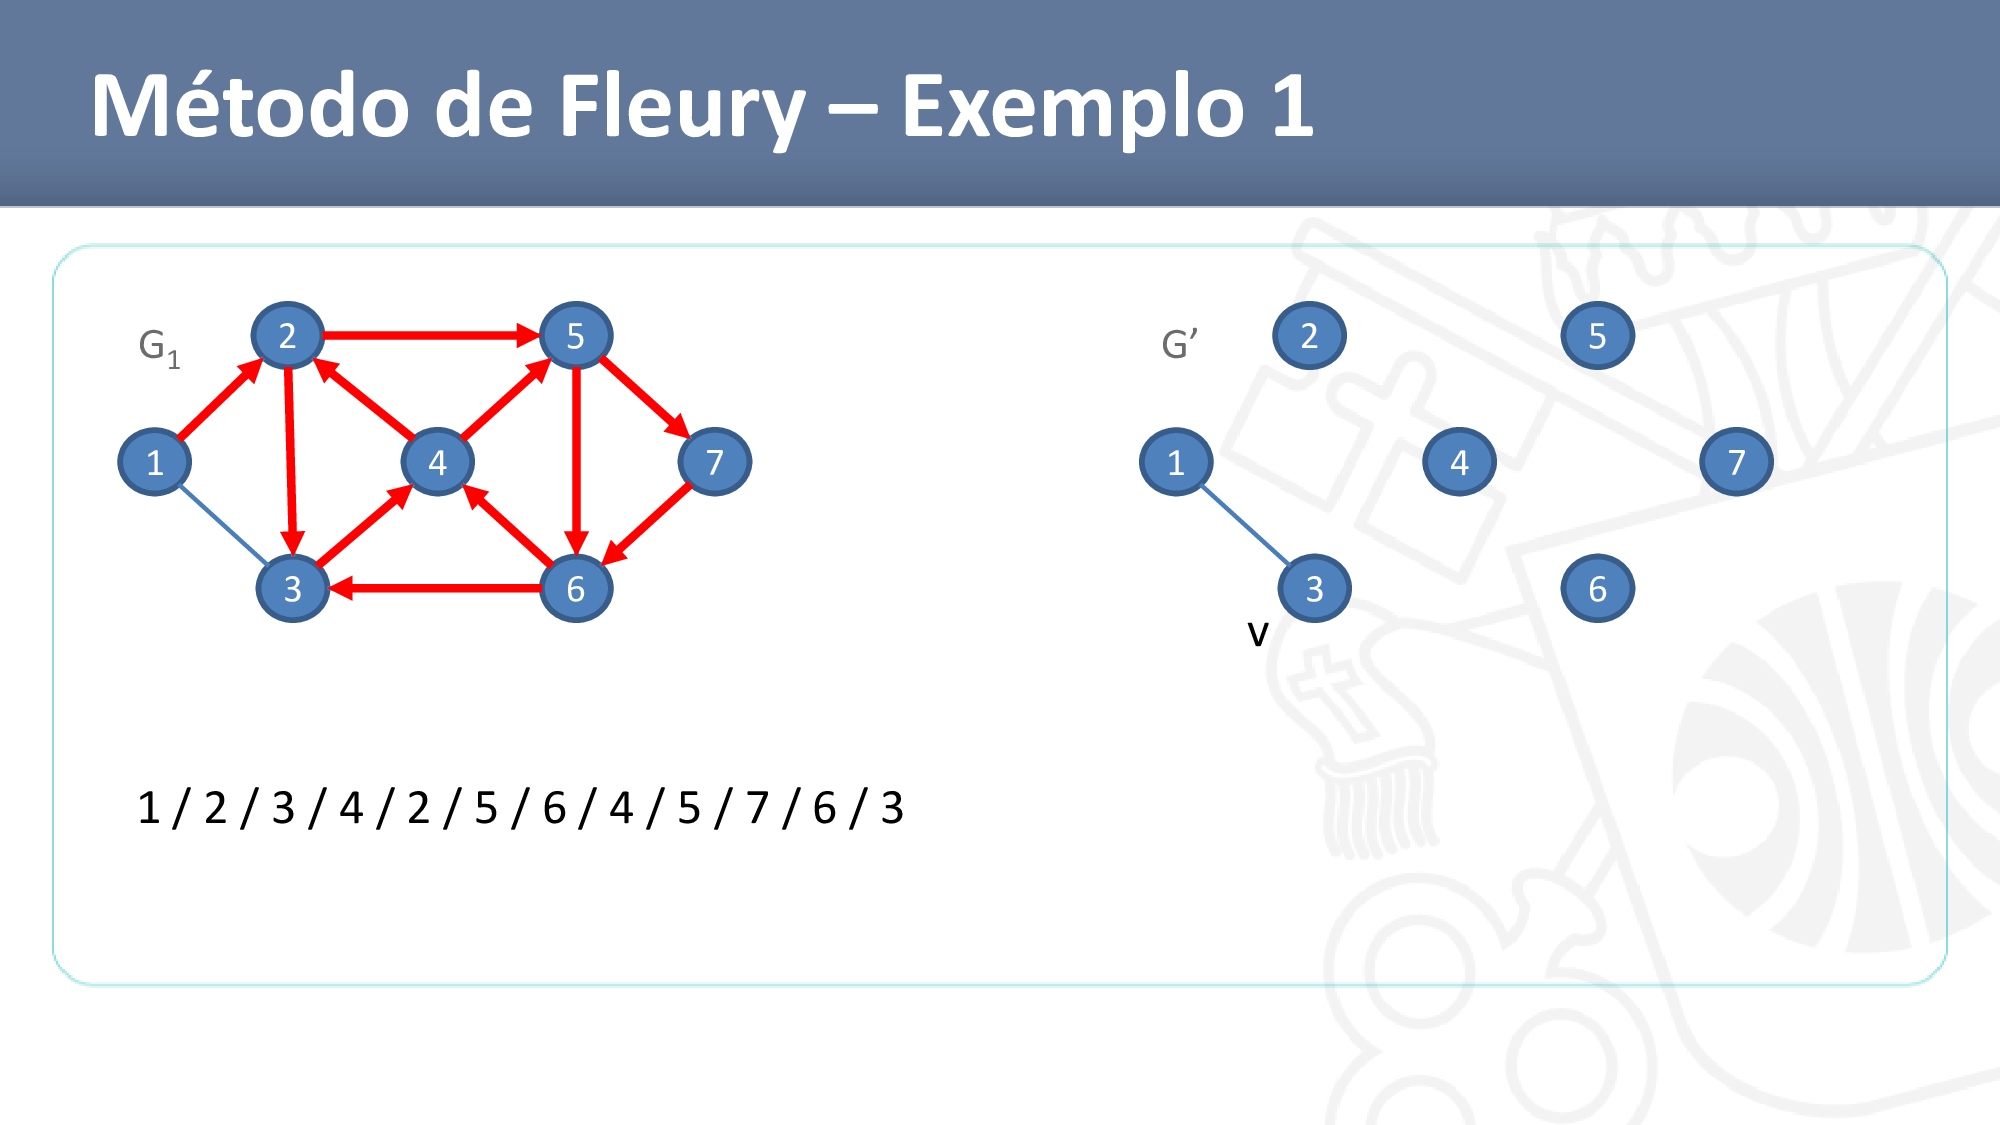
\includegraphics[width=\textwidth]{imagem/graficos/1a1455b7b9174768d1c6a0d41673e79dHTztESkzBtQzsXWu-47.png}
	\end{subfigure}
    \begin{subfigure}{.4\textwidth}
		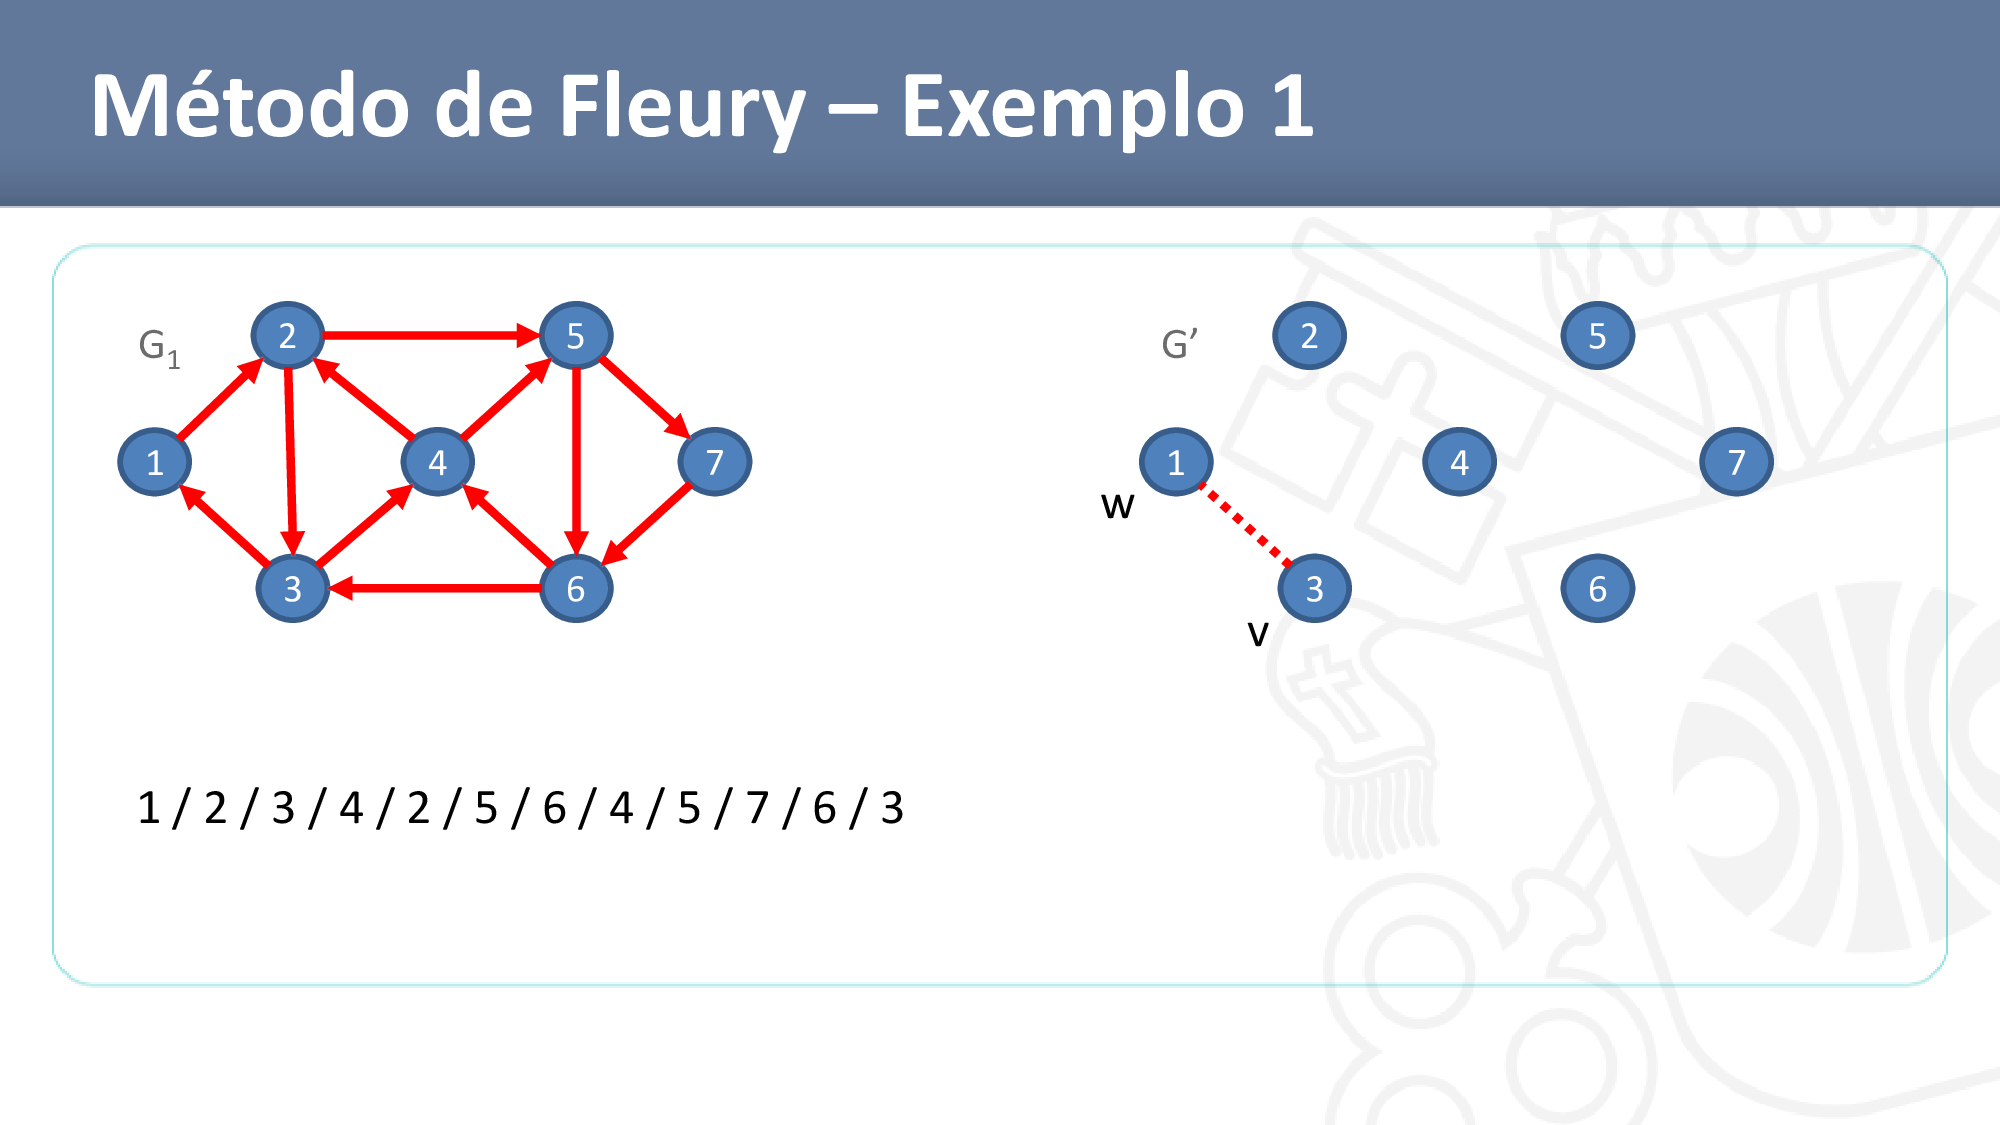
\includegraphics[width=\textwidth]{imagem/graficos/1a1455b7b9174768d1c6a0d41673e79dHTztESkzBtQzsXWu-48.png}
	\end{subfigure}
\end{figure}      
\begin{figure}[htbp]  
    \begin{subfigure}{.4\textwidth}
		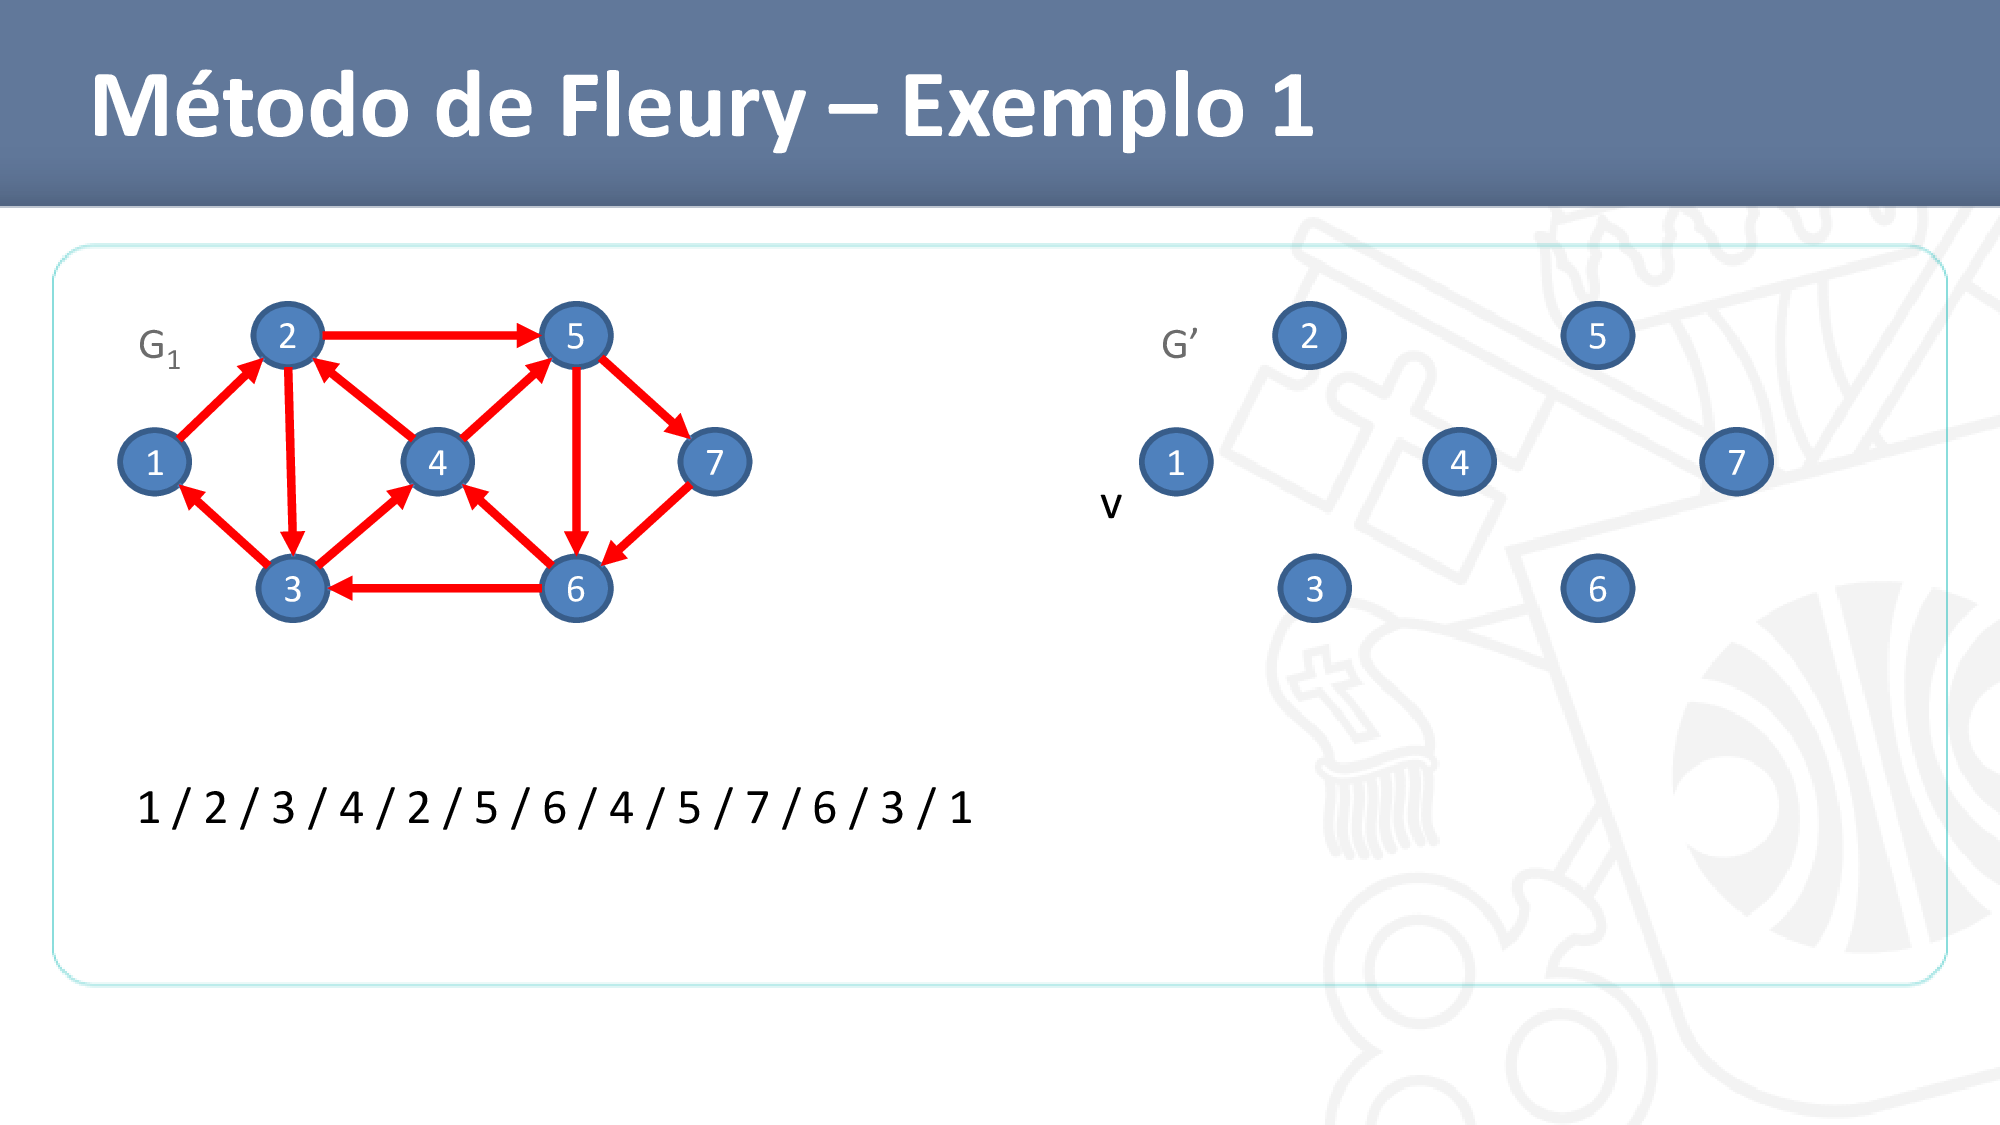
\includegraphics[width=\textwidth]{imagem/graficos/1a1455b7b9174768d1c6a0d41673e79dHTztESkzBtQzsXWu-49.png}
	\end{subfigure}
    \begin{subfigure}{.4\textwidth}
		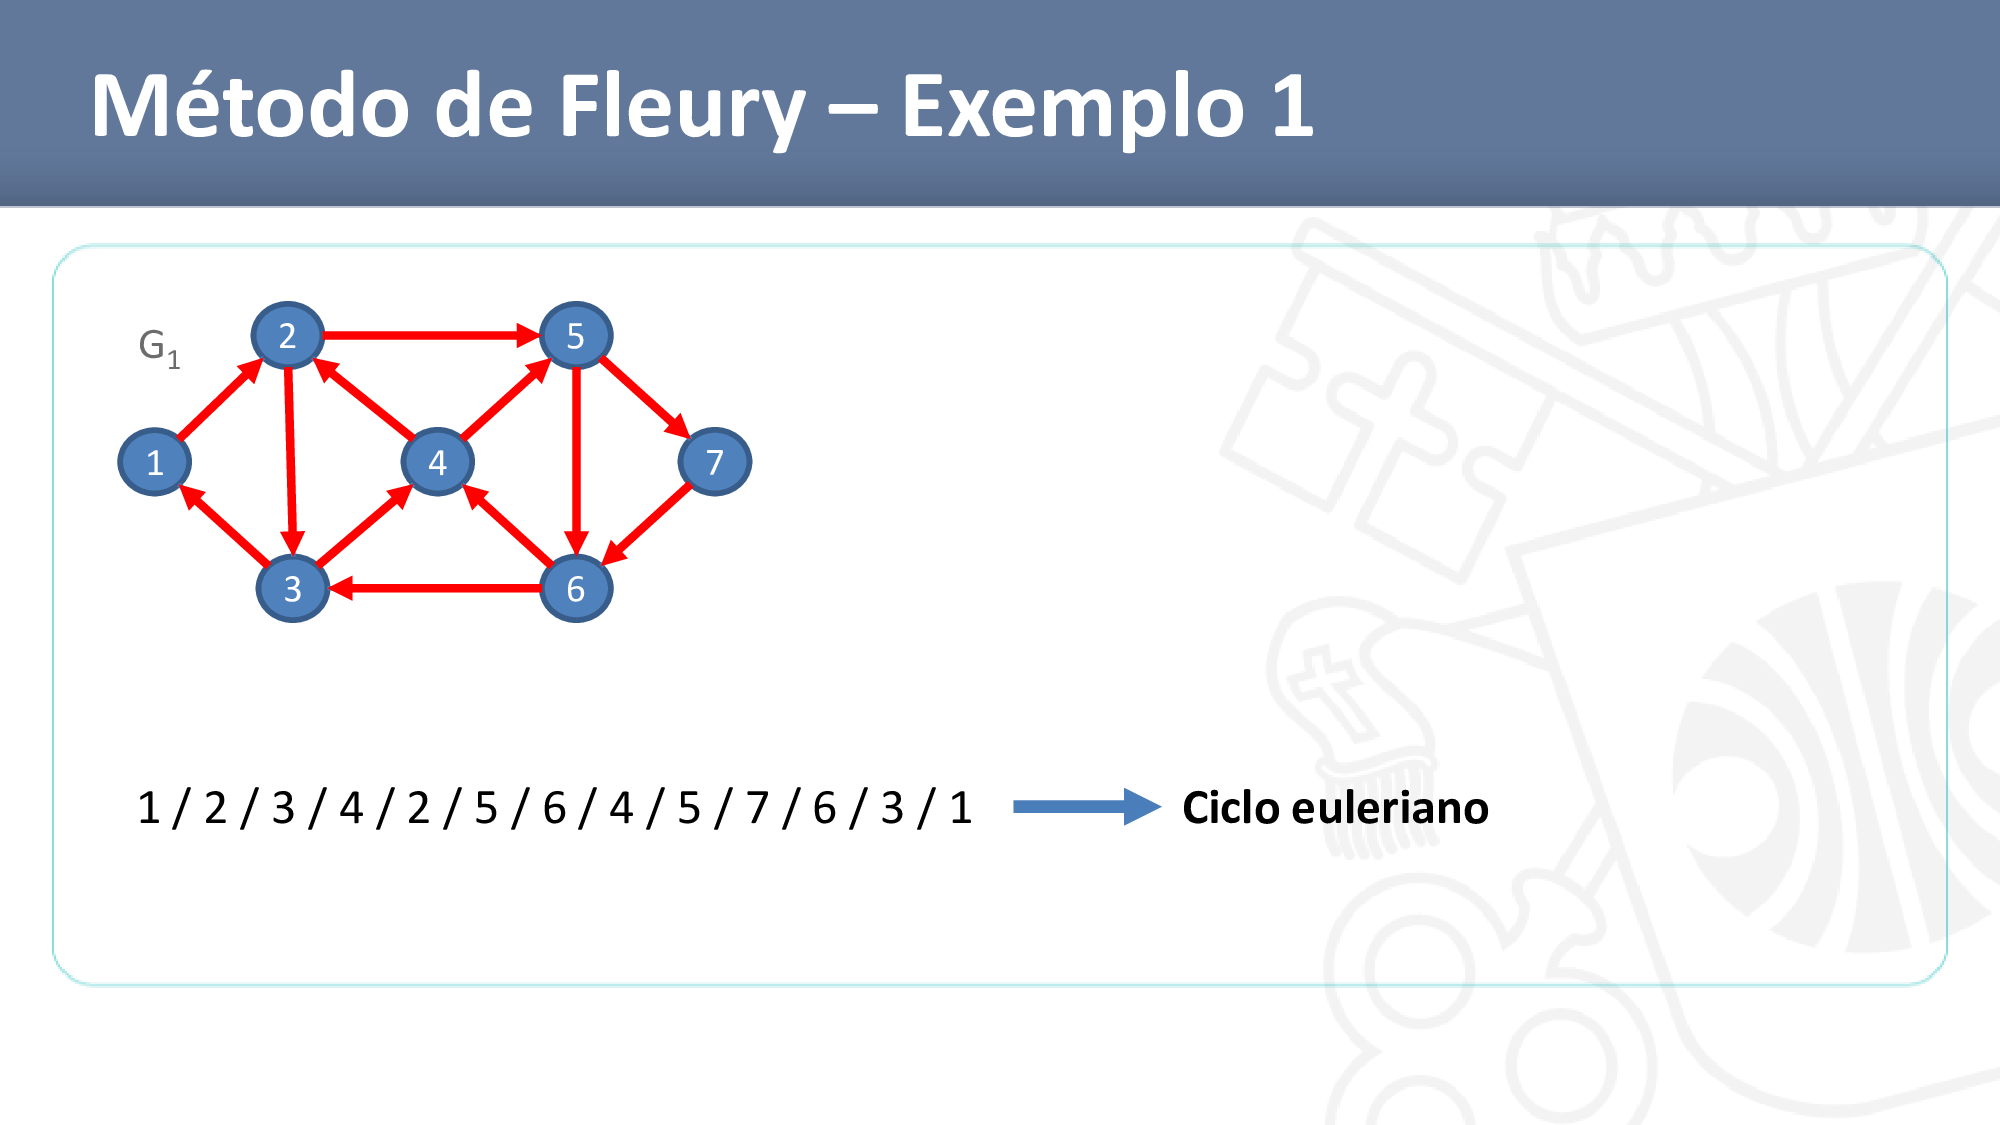
\includegraphics[width=\textwidth]{imagem/graficos/1a1455b7b9174768d1c6a0d41673e79dHTztESkzBtQzsXWu-50.png}
	\end{subfigure}
\end{figure}


% Nome do capítulo
\chapter{Primeiro capítulo de exemplo}
% Label para referenciar
\label{cap1}

% Diminuir espaçamento entre título e texto
\vspace{-1.9cm}

% Texto do capítulo

  % A seguir serão apresentados alguns comandos do LaTex usados comumente para formatar textos de dissertação baseados
  % na normalização da PUC (2011).

  % Para as citações a norma estabelece duas formas de apresentação. A primeira delas é empregada quando a
  % citação aparece no final de um parágrafo. Neste caso, o comando cite é usado para formatar a citação em caixa alta,
  % como é mostrado no exemplo a seguir. \cite{Duato:2002}.

  % Outra forma de apresentação da citação é a que ocorre no decorrer do texto, essa situação é exemplificada na próxima frase.
  % Conforme \citeonline{Bjerregaard:2006}, o estudo mencionado revela progressos no desempenho dos processadores. 
  % Para a formatação da citação em caixa baixa deve ser usado o comando citeonline.

  % Nas citações que aparecem mais de uma referência as mesmas devem ser separadas por vírgulas, como
  % neste exemplo. \cite{Keyes:2008, Zhao:2008, Ganguly:2011}. Se houver necessidade de especificar a página ou que foi
  % realizada uma tradução do texto deve ser feito da seguinte maneira. \cite[p.~2, tradução nossa]{Sasaki:2009}.
  % A citação direta deve ser feita de forma semelhante. ``[...] A carga de trabalho de um sistema pode 
  % ser definida como o conjunto de todas as informações de entrada.''~\cite[p. 160]{Menasce:2002}.

  % O arquivo dissertacao.bib mostra exemplos de representação para vários tipos de referências (artigos de conferências, 
  % periódicos, relatórios, livros, dentre outros). Cada um desses tipos requer uma forma diferente de representação para 
  % que a referência seja formatada conforme as exigências da normalização.

\section{Primeira seção}
\label{secao1}

  % Para gerar a lista de siglas automaticamente deve ser usado o pacote \textit{acronym}. Para tanto, toda vez que uma sigla for mencionada no texto
  % deve ser usado o comando ac\{sigla\}. Dessa forma, se for a primeira ocorrência da sigla a mesma será escrita por extenso
  % conforme descrição feita no arquivo lista-siglas.tex. Caso contrário, somente a sigla será mostrada. Ex

\subsection{Primeira subseção}
  
  % As enumerações devem ser geradas usando o pacote \textit{compactitem}. Cada item deve terminar com um ponto final.
  % Abaixo um exemplo de enumeração é apresentado:

  %   \begin{compactitem}
  %     \item[a)] Coletar e analisar.
  %     \item[b)] Configurar e simular.
  %     \item[c)] Definir a metodologia.
  %     \item[d)] Avaliar o desempenho.
  %     \item[e)] Analisar e avaliar características.
  %   \end{compactitem}

\section{Segunda seção}

  % Para referenciar um capítulo, seção ou subseção basta definir um label para o mesmo e usar o comando ref para referênciá-lo
  % no texto. Exemplo: Como pode ser visto no Capítulo \ref{cap1} ou na Seção \ref{secao1}.
% Nome do capítulo
\chapter{Segundo capítulo de exemplo}
% Label para referenciar
\label{cap2}

% Diminuir espaçamento entre título e texto
\vspace{-1.9cm}

% Texto do capítulo
  
  As figuras devem ser apresentadas pelos comandos abaixo. O parâmetro \textit{width} determina o tamanho que a figura
  será exibida. No parâmetro \textit{caption} o texto que aparece entre colchetes será o exibido no índice de figuras e o texto
  contido entre chaves será exibido na legenda da figura. Para citar a figura o comando ref deve ser usado juntamente
  com o label, como é mostrado nesse exemplo da Figura \ref{fig:ComponentesWiNoC}.

  \begin{figure}[H]
  % Alterar espaçamentos antes e depois do caption
  \setlength{\abovecaptionskip}{0pt}
  \setlength{\belowcaptionskip}{0pt}
  % Caption
  \caption[Principais componentes de WiNoCs]{Principais componentes de WiNoCs}
  \centering
  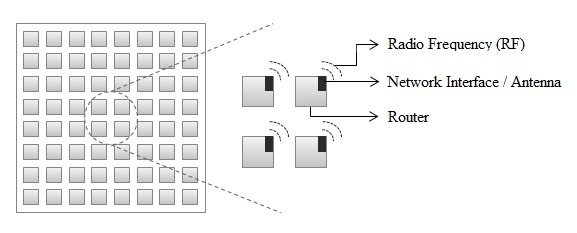
\includegraphics[width=.85\textwidth]{imagem/winoc.jpg}
  % Caption centralizada
  \captionsetup{justification=centering}
  \captionfont{\small{\textbf{\\Fonte: \cite{OliveiraIadis:2011}}}}	
  \label{fig:ComponentesWiNoC}
  \end{figure}


  Os comandos abaixo são usados para apresentação de gráficos. A diferença está apenas na definição do tipo ``grafico`` 
  que permite a adição dos itens no índice de gráficos de forma automática. Os parâmetros são semelhantes aos usados para
  representação de figuras. O parâmetro \textit{width} determina o tamanho do gráfico. O texto entre colchetes 
  no \textit{caption} será o exibido no índice de gráficos e o texto contido entre chaves será exibido na legenda.

\begin{grafico}[H]
  % Alterar espaçamentos antes e depois do caption
  \setlength{\abovecaptionskip}{5pt}
  \setlength{\belowcaptionskip}{0pt}
  % Caption
  \caption[Percentual de pacotes enviados]
	  {Percentual de pacotes enviados}
  \centering
  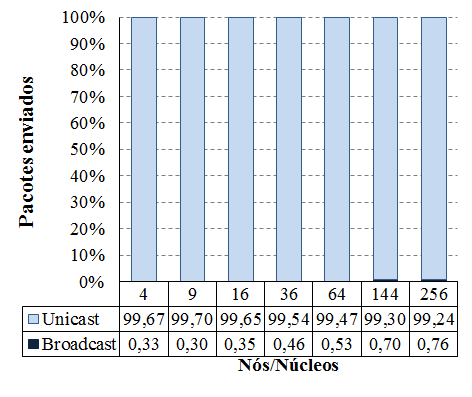
\includegraphics[width=.48\textwidth]{imagem/graficos/grafico_pacotes_enviados_bt.png}
  % Caption centralizada
  \captionsetup[grafico]{justification=centering}
  % Fonte
  \captionfont{\small{\textbf{\\Fonte: Dados da pesquisa}}}
  \end{grafico}

  

Um exemplo de criação de tabela é mostrado a seguir. As colunas são separadas por elementos \& e as linhas por duas barras invertidas. 
  Os comandos \textit{hline} e | definem a criação de linhas e colunas para separar os conteúdos, respectivamente. A tabela pode
  ser referenciada usando o comando ref juntamente com o label, como na Tabela \ref{tab:classesNas}. 

   % Tabela
  \begin{table}[H]
    \centering
    \footnotesize
    % Alterar espaçamentos antes e depois do caption
    \setlength{\abovecaptionskip}{0pt}
    \setlength{\belowcaptionskip}{0pt}
    % Caption
    \caption[Parâmetros definidos por classe]{Parâmetros definidos por classe}
    \label{tab:classesNas}
    % Conteúdo da tabela
    \begin{tabular}{c|c|c|c|c|c|c|c}
	\hline \hline
	\textit{Benchmark} &	Parâmetro &	Classe S &	Classe W &	Classe A &	Classe B &	Classe C &	Classe D \\ 
	\hline \hline
 	BT & \textit{Grid}	& $12^3$	& $24^3$ 	& $64^3$	& $102^3$ 	& $162^3$	& $408^3$ \\ 
	CG & Linhas		& 1400		& 7000 		& 14000 	& 75000 	& 150000 	& 1500000 \\ 
	EP & Pares 		& $2^{24}$	& $2^{25}$	& $2^{28}$	& $2^{30}$	& $2^{32}$	& $2^{36}$ \\
	FT & \textit{Grid}	& $64^3$	& $128^2*32$	& $256^2*128$	& $512*256^2$	& $512^3$	& $2048*1024^2$ \\ 
	IS & Chaves		& $2^{16}$	& $2^{20}$	& $2^{23}$	& $2^{25}$	& $2^{27}$	& $2^{31}$ \\ 
	LU & \textit{Grid}	& $12^3$	& $33^3$	& $64^3$	& $102^3$	& $162^3$	& $408^3$ \\
	MG & \textit{Grid}	& $32^3$	& $128^3$	& $256^3$	& $256^3$	& $512^3$	& $1024^3$ \\ 
	SP & \textit{Grid}	& $12^3$	& $36^3$	& $64^3$	& $102^3$	& $162^3$	& $408^3$ \\
	\hline \hline
    \end{tabular}
    % Fonte
    \captionfont{\small{\textbf{\\Fonte: Adaptado de \cite{Nas:2011}}}}
  \end{table}
% Nome do capítulo
\chapter{Observações importantes}
% Label para referenciar
\label{cap3}

% Diminuir espaçamento entre título e texto
\vspace{-1.9cm}

% Texto do capítulo

  Este documento foi compilado em ambiente linux (Ubuntu 10.04) usando o programa Kile - an Integrated LaTeX Environment - Version 2.0.85.
  Para correta formatação os seguintes arquivos do pacote \textit{abntex} devem ser alterados.

    \begin{compactitem}
      \item[a)] Arquivo abnt.cls

      No Ubuntu o arquivo fica armazenado em \textit{/usr/share/texmf/tex/latex/abntex}.
      Comentar a linha 967: Linha comentada para reduzir o espaçamento entre o topo da página e o título.
      Alterar a linha 1143: Parâmetro alterado de 30pt para -30pt para reduzir o espaçamento entre o top da página e o título do apêndice.
      Alterar a linha 985: Parâmetro alterado de 0pt para -30pt para reduzir o espaçamento entre o top da página e o título.
      Alterar a linha 991: Parâmetro alterado de 45pt para 30pt para reduzir o espaçamento entre o texto e o título.

      \item[b)] Arquivo acronym.sty

      No Ubuntu o arquivo fica armazenado em \textit{/usr/share/texmf-texlive/tex/latex/acronym}.
      Alterar a linha 225: Inserir o separador -- entre acrônimo/descrição e remover o negrito com o \textit{normalfont}.
      %\item[\protect\AC@hypertarget{#1}{\acsfont{\normalfont{#2}}} --] #3 

    \end{compactitem}

% PÓS-TEXTUAIS %%
% Bibliografia no arquivo 'Dissertacao.bib'
% Alterar o título das referências para somente 'Referências'
\renewcommand{\bibname}{Referências}
%\bibliographystyle{abnt-alf}
\bibliography{Referencias}

% Para forçar que os apêndices e anexos comecem no anverso
%\setboolean{@openright}{true}

%\apendice
%\begin{apendice}
%%------------------------------------------------------------------------------------------------------------------------------------------------------
% Reiniciar numeração das figuras que aparecem no apêndice
\setcounter{figure}{0}

\chapter{Primeiro apêndice}
\label{apend:codigoMpe}

% Para diminuir espaçamento entre o título e o texto
\vspace{-1.9cm}

Textos ou documentos elaborados pelo autor, como por exemplo código-fonte.


\lstinputlisting[language=C, label=codigo, caption={Trecho de código modificado}]{pos-texto/codigo.c}
%\end{apendice}

%\anexo
%% Nome do Anexo
\chapter{Primeiro Anexo}

% Para diminuir espa�amento entre o t�tulo e o texto
\vspace{-1.9cm}

% Texto
Textos ou documentos não elaborados pelo autor.

\end{document}